%-----------------------------------------------------------------------------%
\chapter{\babEmpat} \label{chap:analisis}
%-----------------------------------------------------------------------------%%-----------------------------------------------------------------------------%
\section{Pendahuluan}
%-----------------------------------------------------------------------------%
Pada bab ini, analisis korpus data jurnalistik Bahasa Indonesia termutakhir ragam tulis dan lisan dijabarkan melalui beberapa tahap. Kedua korpus dianalisis secara terpisah agar temuan analisis dapat disandingkan untuk melihat perbedaan karakter serta signifikansi perbedaan tersebut antara data ragam tulis dan ragam lisan. Tahap pertama merupakan proses penguraian kalimat dengan metode komputasional berdasarkan dependensinya. Merujuk pada penjelasan dalam Bab 3, penguraian kalimat ini dilakukan dengan bantuan sebuah kerangka kerja yang dapat dilatih ulang untuk pengkategorian token, penguraian lemma, dan penguraian kalimat bernama UDPipe \citep{udpipe2017}. Tahap kedua adalah proses penghitungan untuk mendapatkan nilai Panjang Dependensi (DL) dengan pendekatan yang diadopsi dari penelitian \cite{gildea2010grammars} dan \cite{futrell2015large} serta nilai Rata-rata Jarak Dependensi (MDD) dengan pendekatan yang diadopsi dari penelitian \cite{liu2017dependency}. Kemudian, pada tahap ketiga dilakukan percobaan acak dengan mengadopsi prinsip langkah-langkah \textit{Free Word Order Baseline} \citep{futrell2015large} terhadap tabel yang dihasilkan dari tahap-tahap tersebut. Tahap terakhir melibatkan analisis secara kualitatif terhadap kalimat-kalimat di dalam kedua korpus yang mewakili aspek-aspek temuan penelitian berdasarkan analisis kuantitatif.

Pada tahap pertama, kedua korpus data jurnalistik dipersiapkan untuk dapat diolah dengn metode komputasional. Dalam data ragam lisan ditemukan beberapa ujaran yang bersifat tidak selesai. Karena metode penguraian kalimat belum dapat mengolah ujaran seperti ini, maka ujaran-ujaran tidak selesai dikeluarkan dari korpus terlebih dahulu agar tidak mempengaruhi hasil penghitungan ujaran lainnya. Hasil dari tahap penguraian kalimat ini berupa tabel yang berisi anotasi konstituen-konstituen ujaran seperti contoh pada \tab~\ref{tab:penggalan_kalimat}. Berdasarkan penguraian kalimat ini, kedua korpus memiliki total 19.530 kalimat atau 270.409 konstituen dengan data ragam tulis berjumlah 9311 kalimat atau 162.201 konstituen dan data ragam lisan berjumlah 10.219 kalimat atau 108.208 konstituen. Untuk memastikan kualitas penguraian kalimat dan anotasi yang sesuai, dilakukan tahap tambahan yaitu pemeriksaan secara manual. Berdasarkan pemeriksaan ini, kualitas penguraian kalimat untuk data ragam tulis terbilang sudah bagus, namun pada ragam lisan masih diperlukan pengembangan terutama untuk kata-kata informal atau sehari-hari. Contoh hasil penguraian pada \tab~\ref{tab:penggalan_kalimat} memperlihatkan ujaran "Mengingat fungsi dari telepon seluler tersebut sebagai sarana komunikasi yang berdampak pada peningkatan ekonomi" yang telah diekstraksi menjadi kata-kata yang memiliki anotasi untuk kelas kata serta hubungan antarkonstituennya. 

\begin{center}
\begin{table} \caption{Penggalan penguraian kalimat diambil dari korpus yang dianalisis}\label{tab:penggalan_kalimat}
\begin{tiny}
  \begin{tabulary}{1\textwidth}{| L | L | L | L | L | L | L |}
  \hline
    type & sentence & token & upos & relation & token id & head token id \\ \hline
tulis & Mengingat fungsi dari telepon seluler tersebut sebagai sarana komunikasi yang berdampak pada peningkatan perekonomian & Mengingat & VERB & root & 1 & 0 \\ \hline
tulis & Mengingat fungsi dari telepon seluler tersebut sebagai sarana komunikasi yang berdampak pada peningkatan perekonomian & fungsi & NOUN & obj & 2 & 1 \\ \hline
tulis & Mengingat fungsi dari telepon seluler tersebut sebagai sarana komunikasi yang berdampak pada peningkatan perekonomian & dari & ADP & case & 3 & 4 \\ \hline
tulis & Mengingat fungsi dari telepon seluler tersebut sebagai sarana komunikasi yang berdampak pada peningkatan perekonomian & telepon & NOUN & adl & 4 & 2 \\ \hline
tulis & Mengingat fungsi dari telepon seluler tersebut sebagai sarana komunikasi yang berdampak pada peningkatan perekonomian & seluler & NOUN & compound & 5 & 4 \\ \hline
tulis & Mengingat fungsi dari telepon seluler tersebut sebagai sarana komunikasi yang berdampak pada peningkatan perekonomian & tersebut & DET & det & 6 & 4 \\ \hline
tulis & Mengingat fungsi dari telepon seluler tersebut sebagai sarana komunikasi yang berdampak pada peningkatan perekonomian & sebagai & ADP & case & 7 & 8 \\ \hline
tulis & Mengingat fungsi dari telepon seluler tersebut sebagai sarana komunikasi yang berdampak pada peningkatan perekonomian & sarana & NOUN & adl & 8 & 2 \\ \hline
tulis & Mengingat fungsi dari telepon seluler tersebut sebagai sarana komunikasi yang berdampak pada peningkatan perekonomian & komunikasi & NOUN & compound & 9 & 8 \\ \hline
tulis & Mengingat fungsi dari telepon seluler tersebut sebagai sarana komunikasi yang berdampak pada peningkatan perekonomian & yang & PRON & nsubj & 10 & 11 \\ \hline
tulis & Mengingat fungsi dari telepon seluler tersebut sebagai sarana komunikasi yang berdampak pada peningkatan perekonomian & berdampak & VERB & acl:relcl & 11 & 8 \\ \hline
tulis & Mengingat fungsi dari telepon seluler tersebut sebagai sarana komunikasi yang berdampak pada peningkatan perekonomian & pada & ADP & case & 12 & 13 \\ \hline
tulis & Mengingat fungsi dari telepon seluler tersebut sebagai sarana komunikasi yang berdampak pada peningkatan perekonomian & peningkatan & NOUN & obl & 13 & 11 \\ \hline
tulis & Mengingat fungsi dari telepon seluler tersebut sebagai sarana komunikasi yang berdampak pada peningkatan perekonomian & perekonomian & NOUN & compound & 14 & 13 \\ 
\hline
  \end{tabulary}  
\end{tiny}
\end{table}
\end{center}

Untuk memudahkan dalam analisis kualitatif dan melihat secara dekat tautan-tautan dependensi yang terbentuk pada sebuah ujaran, visualisasi seperti pada \pic~\ref{fig:visualisasi_penguraian} dilakukan secara terpisah. Proses visualisasi ini hanya dilakukan pada ujaran-ujaran yang akan dilihat lebih rinci sebagai contoh yang mewakili hasil temuan dengan bantuan kerangka kerja UDPipe \citep{udpipe2017}. Pada kalimat contoh ini, terlihat bahwa ujaran memiliki akar verbal 'mengingat' yang simpai pusatnya hanya terdiri dari satu tautan, yaitu 'mengingat fungsi' dengan hubungan tautan $obj$ atau obyek. Penelitian ini merupakan penelitian terhadap penggunaan bahasa secara nyata (\textit{real utterance}). Sehingga,  meskipun beberapa ujaran yang ditemukan terlihat seperti klausa terikat saja, atau tampak seperti ujaran yang tidak lengkap, semua ujaran tetap dianalisis tanpa koreksi atau manipulasi.

\begin{figure}
	\centering 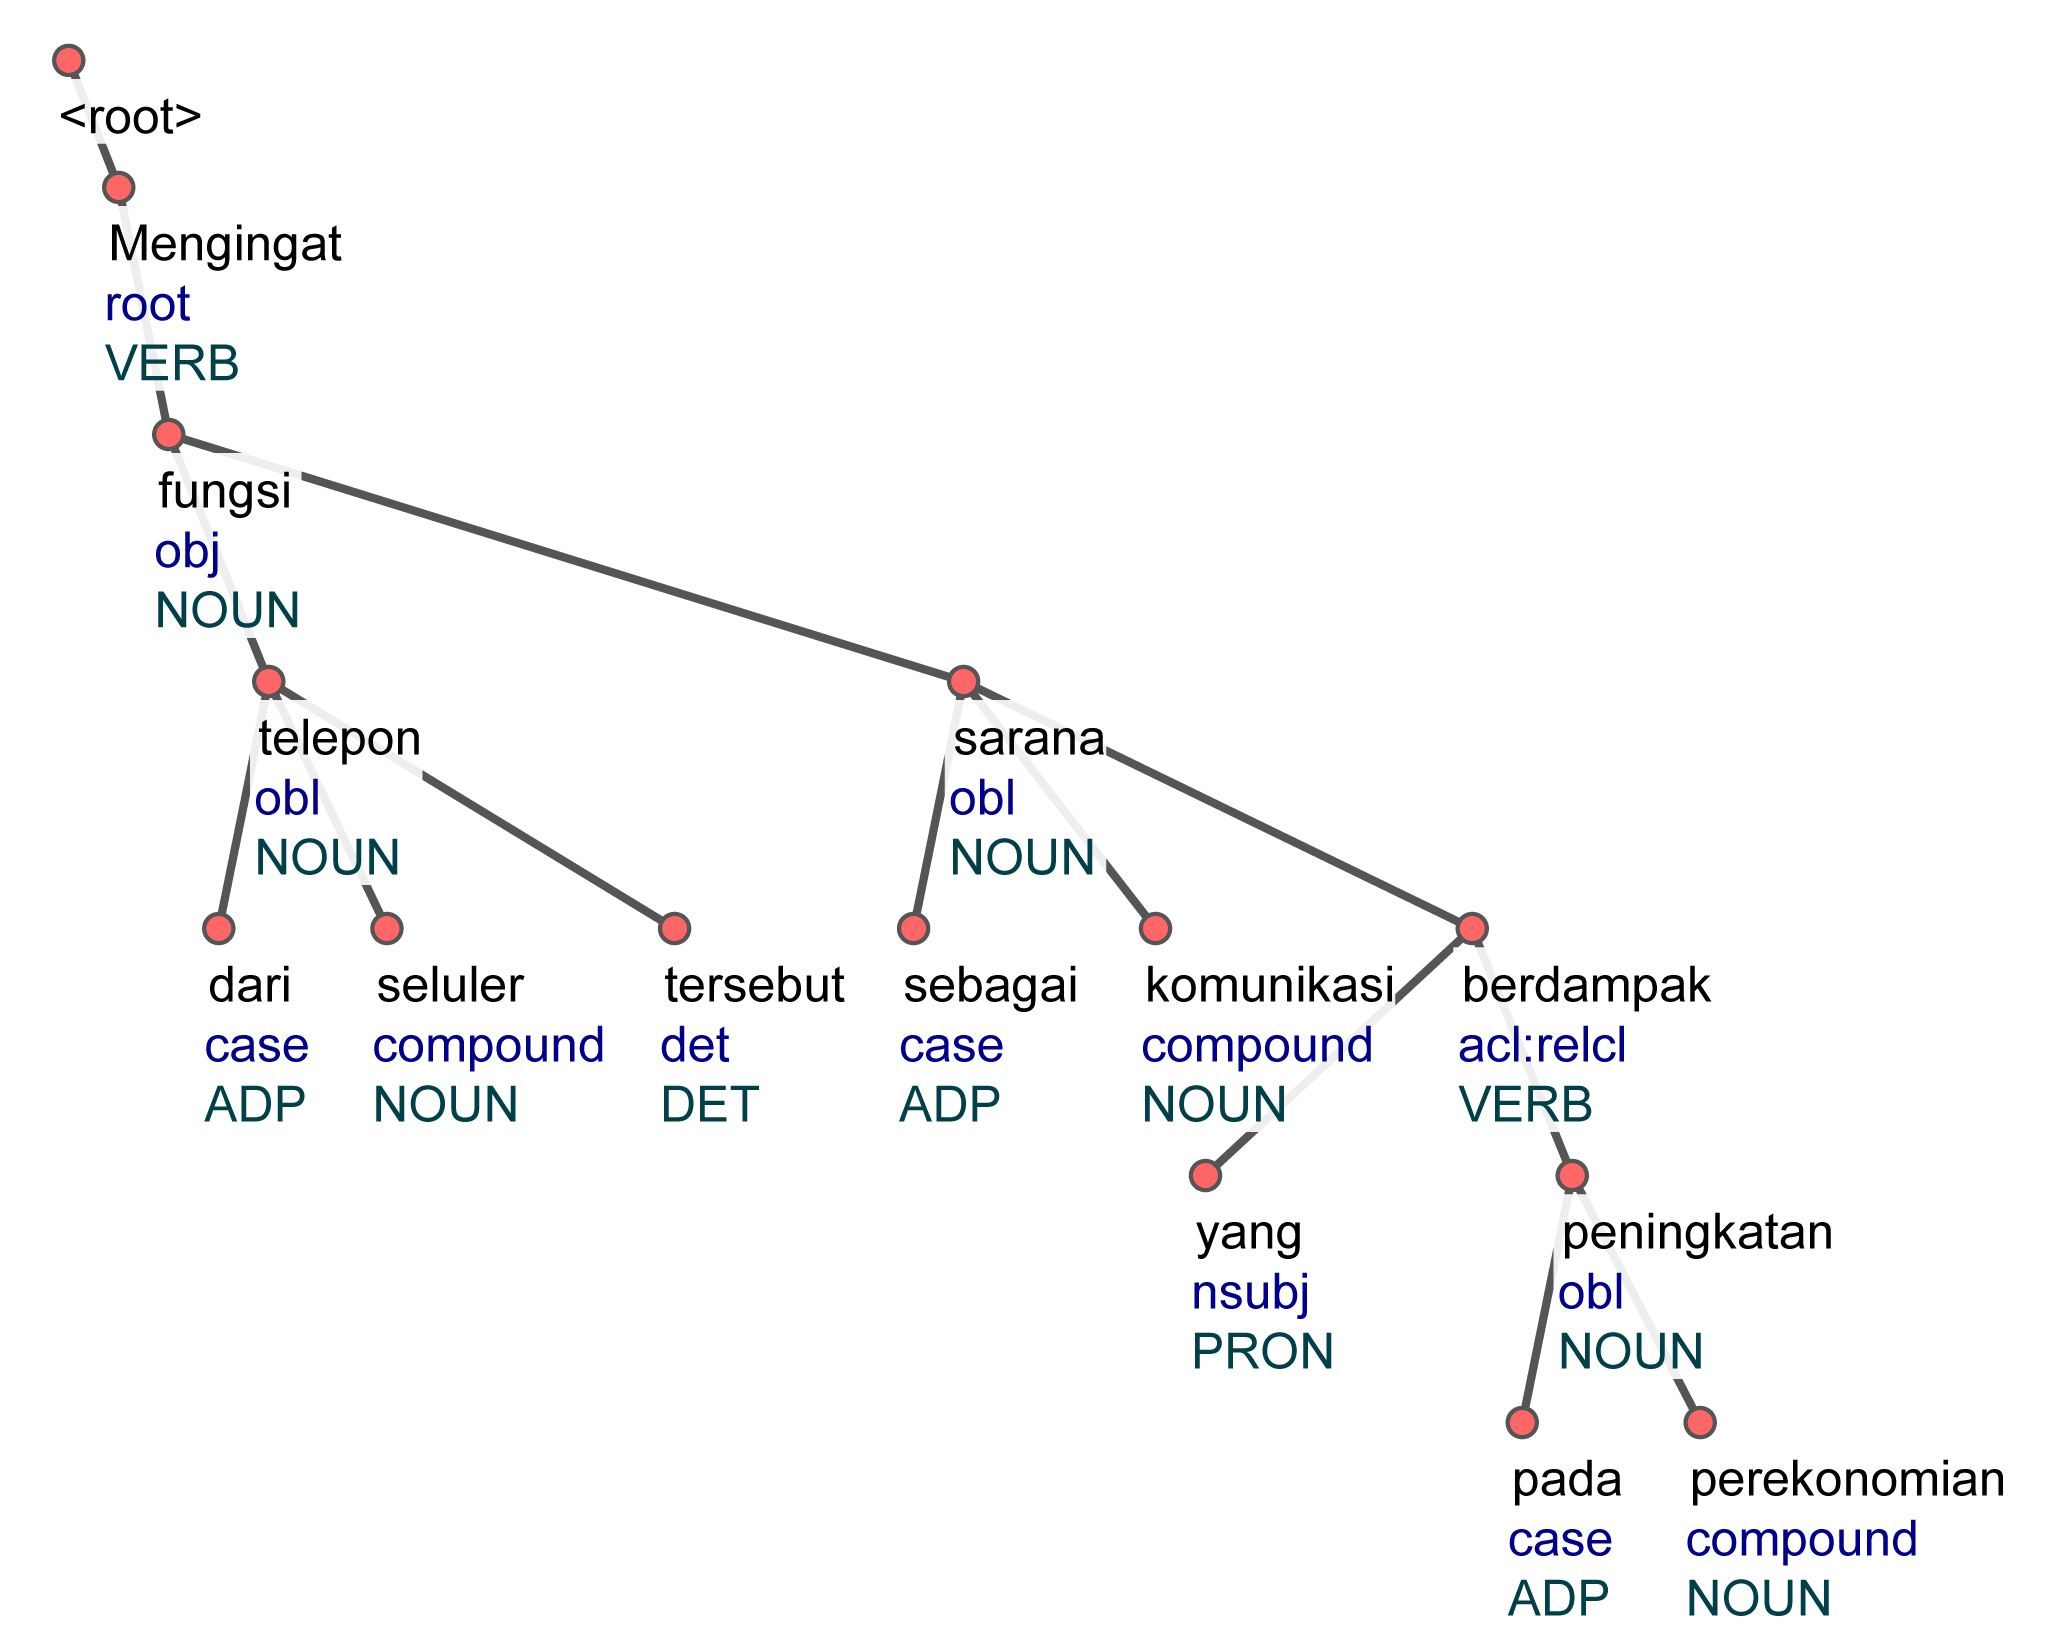
\includegraphics[width=0.8
	\textwidth] {pics/visualisasi_penguraian.jpg} 
	\caption{Contoh visualisasi penguraian kalimat berdasarkan dependensi} 
\label{fig:visualisasi_penguraian} \end{figure}

Tahap selanjutnya melibatkan proses anotasi nilai-nilai yang berkaitan dengan tautan dependensi sebuah ujaran pada tabel hasil penguraian kalimat. Anotasi ini dihasilkan melalui penghitungan nilai DL dan penghitungan nilai MDD seperti yang dijabarkan pada Bab 2 dan rumus penghitungan yang dijabarkan pada Bab 3. DL menekankan pada total jumlah dependensi yang didapatkan dari semua tautan dependensi dalam sebuah ujaran, sedangkan MDD menekankan pada rata-rata jarak dependensi antara dua konstituen dalam sebuah ujaran. Meskipun memiliki prinsip mendasar yang serupa, saya berasumsi ada perbedaan informasi yang berarti antara kedua pendekatan ini sehingga keduanya digunakan dalam penelitian ini. Eksplorasi perbedaan pendekatan DL dan MDD serta penentuan pendekatan mana yang lebih optimal dalam mengilustrasikan efisiensi memori kerja melalui struktur sintaksis ujaran bukan merupakan fokus penelitian ini, namun hasil penerapan kedua pendekatan dalam penelitian ini dapat berkontribusi dalam menunjukkan pada kondisi mana kedua pendekatan tersebut berbeda. \tab~\ref{tab:dl_mdd} merupakan tabel hasil anotasi terhadap salah satu kalimat di dalam korpus data.

\begin{center}
\begin{table} \caption{Penggalan penguraian kalimat diambil dari korpus yang dianalisis}\label{tab:dl_mdd}
\begin{tiny}
  \begin{tabulary}{1\textwidth}{| L | L | L | L | L | L | L | L |}
  \hline
type & sentence & dl & sum\textunderscore dl & dl\textunderscore positive & dl\textunderscore negative & mdd \\ \hline
tulis & Mengingat fungsi dari telepon seluler tersebut sebagai sarana komunikasi yang berdampak pada peningkatan perekonomian & 0 & 0 & 0 & 0 & 0.00 \\ \hline
tulis & Mengingat fungsi dari telepon seluler tersebut sebagai sarana komunikasi yang berdampak pada peningkatan perekonomian & 1 & 1 & 1 & 0 & 0.08 \\ \hline
tulis & Mengingat fungsi dari telepon seluler tersebut sebagai sarana komunikasi yang berdampak pada peningkatan perekonomian & -1 & 2 & 1 & -1 & 0.15 \\ \hline
tulis & Mengingat fungsi dari telepon seluler tersebut sebagai sarana komunikasi yang berdampak pada peningkatan perekonomian & 2 & 4 & 3 & -1 & 0.31 \\ \hline
tulis & Mengingat fungsi dari telepon seluler tersebut sebagai sarana komunikasi yang berdampak pada peningkatan perekonomian & 1 & 5 & 4 & -1 & 0.38 \\ \hline
tulis & Mengingat fungsi dari telepon seluler tersebut sebagai sarana komunikasi yang berdampak pada peningkatan perekonomian & 2 & 7 & 6 & -1 & 0.54 \\ \hline
tulis & Mengingat fungsi dari telepon seluler tersebut sebagai sarana komunikasi yang berdampak pada peningkatan perekonomian & -1 & 8 & 6 & -2 & 0.62 \\ \hline
tulis & Mengingat fungsi dari telepon seluler tersebut sebagai sarana komunikasi yang berdampak pada peningkatan perekonomian & 6 & 14 & 12 & -2 & 1.08 \\ \hline
tulis & Mengingat fungsi dari telepon seluler tersebut sebagai sarana komunikasi yang berdampak pada peningkatan perekonomian & 1 & 15 & 13 & -2 & 1.15 \\ \hline
tulis & Mengingat fungsi dari telepon seluler tersebut sebagai sarana komunikasi yang berdampak pada peningkatan perekonomian & -1 & 16 & 13 & -3 & 1.23 \\ \hline
tulis & Mengingat fungsi dari telepon seluler tersebut sebagai sarana komunikasi yang berdampak pada peningkatan perekonomian & 3 & 19 & 16 & -3 & 1.46 \\ \hline
tulis & Mengingat fungsi dari telepon seluler tersebut sebagai sarana komunikasi yang berdampak pada peningkatan perekonomian & -1 & 20 & 16 & -4 & 1.54 \\ \hline
tulis & Mengingat fungsi dari telepon seluler tersebut sebagai sarana komunikasi yang berdampak pada peningkatan perekonomian & 2 & 22 & 18 & -4 & 1.69 \\ \hline
tulis & Mengingat fungsi dari telepon seluler tersebut sebagai sarana komunikasi yang berdampak pada peningkatan perekonomian & 1 & 23 & 18 & -5 & 1.77 \\ \hline
  \end{tabulary}  
\end{tiny}
\end{table}
\end{center}

\tab~\ref{tab:dl_mdd} memperlihatkan penghitungan nilai DL dan MDD untuk kalimat 'Mengingat fungsi dari telepon seluler tersebut sebagai sarana komunikasi yang berdampak pada peningkatan perekonomian'. Dengan jumlah konstituen 14, kalimat ini memiliki nilai DL 23 dan MDD 1,77. Hasil ini menunjukkan semua nilai tautan dependensi (total Jarak Dependensi atau DD antarkonstituen) dalam ujaran tersebut berjumlah 23 dengan rata-rata jarak dependensi antara dua konstituen yang memiliki jarak tautan langsung sejauh 1,77 konstituen. Pada tabel tersebut terlihat bahwa nilai DL juga dipisahkan menjadi dua berdasarkan arahnya. Nilai DL positif menggambarkan kondisi \textit{head-initial} yang berarti konstituen terikat (\textit{dependant}) direalisasikan setelah akar atau induk (\textit{root/head}). Sebaliknya, nilai DL negatif menggambarkan kondisi \textit{head-final} yang berarti konstituen terikat direalisasikan sebelum akar atau induk. Analisis hubungan nilai DL positif dan negatif ini memiliki dua bagian. Bagian pertama melihat tautan antara dua konstituen yang memiliki tautan langsung tanpa memperhitungkan posisi frasa atau klausa kedua konstituen tesebut. Analisis bagian kedua melihat tautan antara dua konstituen di mana salah satu konstituen tersebut adalah akar verbal (simpai pusat) dan menganggap semua simpai cabang konstituen tersebut mengikuti nilainya. Pada kalimat kompleks yang memiliki lebih dari satu klausa, tautan dependensi utama ini dapat membawa satu klausa atau lebih di dalamnya. Sebagai contoh, jika terdapat satu tautan dependensi utama yang negatif, dan dalam simpai cabang tersebut terdapat dua klausa, maka kedua klausa tersebut harus disimpan di dalam memori kerja terlebih dahulu hingga akar direalisasikan. Sehingga, posisi simpai cabang menentukan bagaimana seluruh informasi yang dikandungnya diproses. Analisis ini berangkat dari asumsi bahwa Bahasa Indonesia cenderung memilih bentuk tautan \textit{head-initial} yang diambil dari indikasi dari teori struktur frasa yang mengungkapkan banyaknya kondisi di mana induk akan mendahului konstituen terikatnya (\citealp{kridalaksana2002struktur, sneddon2010indonesian}).

Berikutnya, langkah yang dilakukan setelah mendapatkan tabel hasil penguraian ini adalah percobaan acak dengan mengadopsi prinsip langkah-langkah algoritma acak \textit{Free Word Order Baseline} \citep{futrell2015large}. \textit{Free Word Order Baseline} merupakan pendekatan yang dilakukan untuk \cite{futrell2015large} dalam menguji hipotesis adanya Pengurangan Panjang Dependensi (DLM). Pada tahap ini tidak dilakukan perbandingan untuk menguji hipotesis Pengurangan Jarak Dependensi (DDM) karena variabel pembagi, yang dalam hal ini adalah jumlah tautan, tidak berubah sehingga akan menghasilkan gambaran yang serupa dengan uji hipotesis DLM. Dari ujaran-ujaran yang telah diurai, percobaan ini menghasilkan 100 kombinasi struktur ujaran dengan mempertahankan tautan dependensi sesuai hasil observasi. \pic~\ref{fig:percobaan_acak} memperlihatkan tiga contoh hasil percobaan acak terhadap kalimat 'Sama, nanti pecahannya kita lihat' dan perbedaan nilai DL yang didapatkan tiga kombinasi struktur lainnya. Percobaan acak ini dilakukan terhadap semua ujaran yang berada pada kategori jumlah konstituen dengan frekuensi terbanyak. Berdasarkan klasifikasi kalimat terhadap kedua korpus data dan tahap pertama analisis, frekuensi jumlah konstituen terbanyak pada setiap klasifikasi kalimat adalah 10 konstituen (ragam tulis) dan 5 konstituen (ragam lisan) untuk klasifikasi kalimat pendek (\textless= 10 konstituen), 14 konstituen (ragam tulis) dan 12 konstituen (ragam lisan) untuk klasifikasi kalimat menengah (11-20 konstituen), serta 21 konstituen (ragam tulis) dan 22 konstituen (ragam lisan) untuk klasifikasi kalimat panjang (\texgreater 20 konstituen). 

\begin{figure}
	\centering 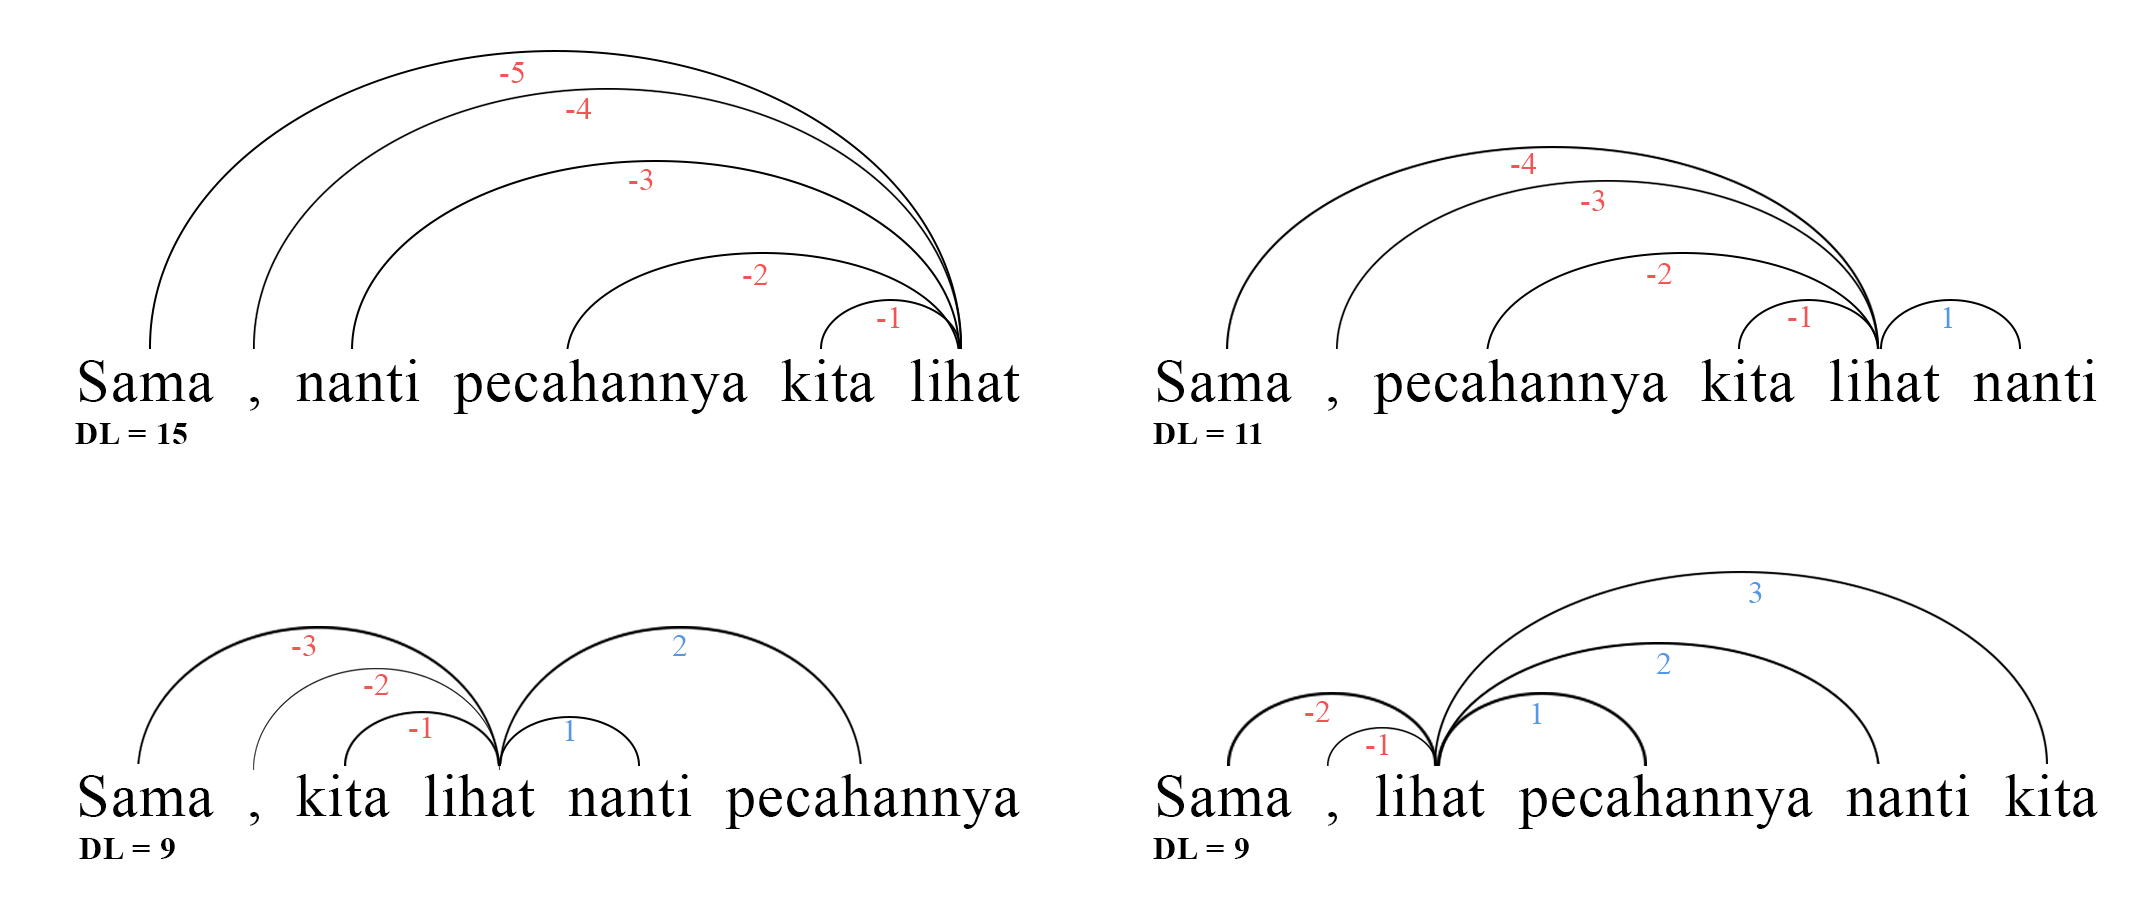
\includegraphics[width=0.8
	\textwidth] {pics/percobaan_acak.jpg} 
	\caption{Contoh hasil percobaan acak} 
\label{fig:percobaan_acak} 
\end{figure}

Merujuk pada penjelasan dalam tinjauan pustaka pada Bab 2, bahasa Indonesia memiliki urutan kata yang cenderung bebas, dan beberapa kasus menunjukkan pertukaran kata maupun klausa tidak mengubah makna ujaran \citep{sneddon2010indonesian}. Dalam penelitiannya, \cite{futrell2015large} menunjukkan kedekatan hasil data observasi bahasa Indonesia dengan nilai DL minimum menggunakan pendekatan ini untuk korpus data yang berisi tulisan penelitian. Temuan ini memberikan indikasi bahwa penerapan kebebasan urutan kata tidak hanya terjadi pada ujaran yang dianggap gramatikal, tetapi terutama pada penggunaan bahasa secara nyata dalam kehidupan sehari-hari (data penampilan linguistik). Kebebasan terhadap aturan ini dan asumsi bahwa penutur bahasa Indonesia memanfaatkan kebebasan ini merupakan dasar utama pemilihan pendekatan \textit{Free Word Order Baseline}. Hal ini dikarenakan pendekatan tersebut menghasilkan hasil kombinasi struktur ujaran yang paling minimum dan maksimum sehingga sangat menarik untuk melihat posisi \textit{real utterance} yang didapat melalui observasi terhadap kemungkinan-kemungkinan kombinasi struktur yang terbentuk. 

Tahap terakhir dari analisis penelitian ini merupakan analisis kualitatif untuk melihat perilaku valensi konstituen yang difokuskan pada valensi verbal pada simpai pusat ujaran. Verba sebagai akar ujaran ditemukan sebanyak 84,67\% atau sebanyak 7884 ujaran pada data ragam tulis dan 69,26\% atau sebanyak 7078 ujaran pada data ragam lisan sehingga menjadikan bentuk ini mayoritas dalam kedua korpus data. Analisis ini dilakukan untuk melihat adanya strategi yang menyebabkan terjadinya DLM dan DDM pada level paling utama (simpai pusat) serta perbedaan karakter yang mungkin muncul antara kedua jenis ragam bahasa. Analisis kualitatif juga dilakukan pada temuan yang didapat pada tahap-tahap sebelumnya untuk menguraikan struktur ujaran yang mungkin memberikan informasi lebih mengenai kecenderungan penutur dalam membentuk ujaran yang efisien dari segi dependensi.

%-----------------------------------------------------------------------------%
\section{Panjang Dependensi (DL) dan Rata-rata Jarak Dependensi (MDD) antara data jurnalistik ragam lisan dan tulis}
%-----------------------------------------------------------------------------%
Pada analisis penelitian ini, kedua pendekatan untuk menghitung nilai DL dan nilai MDD digunakan karena diduga masing-masing memberikan informasi yang berbeda atau menunjukkan perbedaan nilai pada kondisi tertentu. Kedua penghitungan ini dilakukan terhadap setiap ujaran dalam korpus data jurnalistik ragam lisan dan tulis. Secara garis besar, ada perbedaan yang cukup terlihat dalam kedua paparan grafik nilai DL dan nilai MDD antara korpus data ragam tulis dan data ragam lisan.

%-----------------------------------------------------------------------------%
\subsection{Perbandingan Panjang Dependensi (DL) antara data jurnalistik ragam lisan dan tulis}
%-----------------------------------------------------------------------------%
Pada pendekatan penghitungan Panjang Dependensi (DL) yang diadopsi dari penelitian \cite{futrell2015large}, seluruh nilai tautan dependensi dalam sebuah ujaran dijumlahkan sehingga nilai DL yang dihasilkan cukup sensitif dan berbanding linear dengan jumlah konstituen dalam ujaran. Pada \pic~\ref{fig:lisantulis_DL} dapat dicermati bahwa terjadi perubahan pada kedua garis regresi. Perbandignan umum ini dilakukan tanpa melihat lebih dalam persebaran data terkait jumlah konstituen dalam ujaran atau tanpa memperhitungkan klasifikasi panjang kalimat. Berdasarkan grafik nilai DL ini, terlihat bahwa mayoritas jumlah konstituen dalam kalimat pada kedua korpus data berada di bawah 40 konstituen. Pada area di bawah 40 konstituen, garis regresi data ragam tulis berada di bawah garis regresi data ragam lisan. Namun, pada area di atas 40 konstituen, garis regresi menunjukkan perbandingan terbalik secara drastis. Secara umum, rata-rata nilai DL adalah 42,61 untuk data ragam tulis dan 24,36 untuk data ragam lisan. 

Tanpa memperhitungkan klasifikasi panjang kalimat, hasil tersebut menunjukkan adanya kecenderungan yang signifikan bahwa ragam lisan akan menghasilkan jumlah nilai tautan dependensi yang lebih kecil. Hal ini berarti ada indikasi bahwa data ragam lisan menunjukkan efisiensi yang lebih tinggi dibandingkan data ragam tulis dilihat dari segi total nilai dependensi dalam sebuah ujaran. Akan tetapi, seperti yang terlihat pada garis regresi yang terbentuk, hingga panjang kalimat 40 konstituen, garis regresi data ragam tulis terus berada di bawah garis regresi ragam lisan dan terjadi pemusatan data pada panjang kalimat yang mendekati minimum untuk data ragam lisan. Hal ini menunjukkan bahwa dugaan awal ini harus dicermati lebih dalam dengan melihat klasifikasi panjang kalimat yang mungkin akan memberikan informasi tambahan lain yang lebih menentukan keakuratan hasil uji hipotesis. 

\begin{figure}
	\centering 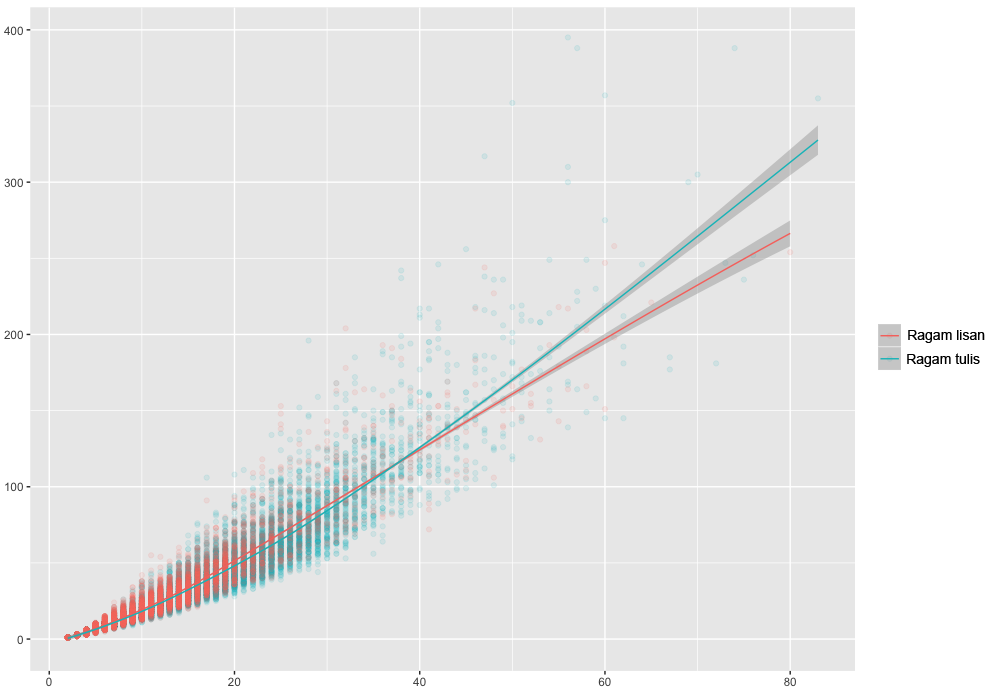
\includegraphics[width=1
	\textwidth] {pics/lisantulis_DL.png} 
	\caption{Grafik nilai DL data ragam tulis dan lisan} 
\label{fig:lisantulis_DL} 
\end{figure}

%-----------------------------------------------------------------------------%
\subsection{Perbandingan Rata-rata Jarak Dependensi (MDD) antara data jurnalistik ragam lisan dan tulis}
%-----------------------------------------------------------------------------%
Berbeda dengan penghitungan nilai DL, Rata-rata Jarak Dependensi (MDD) didapatkan dengan membagi total nilai tautan dependensi dalam sebuah ujaran dengan jumlah tautan itu sendiri. Penghitungan ini menghasilkan perkiraan rata-rata jarak dependensi satu (1) tautan dalam sebuah ujaran sehingga menggambarkan pada umumnya sejauh apa jarak relasi semantik antar dua konstituen. Seperti \pic~\ref{fig:lisantulis_DL}, \pic~\ref{fig:lisantulis_MDD} merupakan paparan nilai MDD untuk semua ujaran pada kedua korpus data (ragam tulis dan lisan). Nilai MDD, seperti yang dikemukakan oleh \cite{liu2017dependency}, tidak terlalu sensitif terhadap jumlah konstituen karena merupakan nilai rata-rata per tautan. Meskipun begitu, berdasarkan grafik nilai MDD ini, pada data dengan jumlah konstituen di bawah 10 nilai MDD masih menunjukkan hasil yang sangat linier terhadap jumlah konstituen. Hal ini berarti mengindikasikan bahwa pada panjang konstituen yang pendek, MDD memiliki tingkat sensitivitas yang lebih tinggi.

Apabila nilai DL memberikan gambaran umum mengenai kompleksitas sebuah ujaran karena hanya fokus terhadap total nilai, nilai MDD dapat lebih memberikan ilustrasi kerja kognisi yang tercermin pada relasi dua buah konstituen di mana untuk kedua konstituen dapat diproses, salah satu harus menunggu yang lain untuk direalisasikan. Pada \pic~\ref{fig:lisantulis_MDD}, dapat disimpulkan bahwa garis regresi untuk korpus data ragam tulis juga berada di bawah garis regresi korpus data ragam lisan dengan panjang kalimat di bawah 40 konstituen namun berbanding terbalik setelah 40 konstituen. Temuan ini menunjukkan konsistensi antara nilai DL dan nilai MDD yang sama-sama menunjukkan bahwa hingga jumlah setidaknya 40 konstituen, kalimat-kalimat dalam data ragam lisan menunjukkan efisiensi yang lebih tinggi dari segi dependensi dibandingkan data ragam tulis. Rata-rata nilai MDD yang didapat dari seluruh ujaran adalah 2,05 konstituen untuk data ragam lisan dan 2,35 konstituen untuk data ragam tulis. Seperti pada catatan grafik nilai DL sebelumnya, nilai ini tidak memperhitungkan klasifikasi panjang kalimat dan pemusatan data ragam tulis pada panjang kalimat yang mendekati minimum juga patut diperhitungkan.

\begin{figure}
	\centering 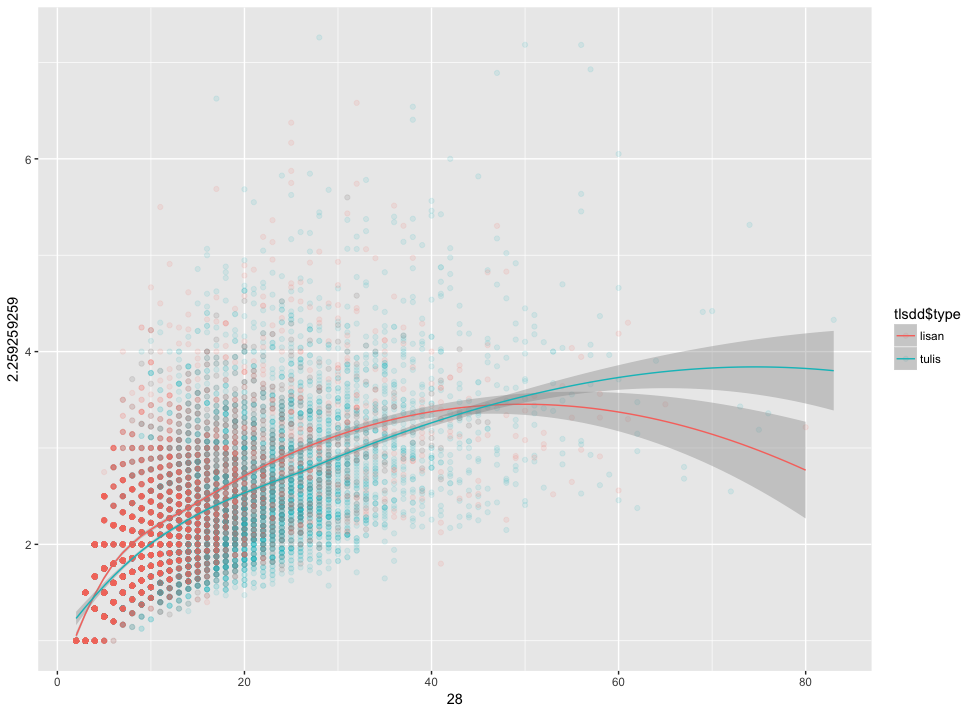
\includegraphics[width=1
	\textwidth] {pics/lisantulis_MDD.png} 
	\caption{Grafik nilai MDD data ragam tulis dan lisan} 
\label{fig:lisantulis_MDD} 
\end{figure}

%%-----------------------------------------------------------------------------%
\section{Perbandingan data hasil observasi dengan hasil percobaan acak}
%%-----------------------------------------------------------------------------%
Setelah mendapatkan gambaran umum mengenai nilai DL dan MDD untuk kedua korpus data, percobaan acak terhadap kedua korpus data dilakukan untuk melihat apakah ujaran-ujaran dalam data hasil observasi, baik ragam tulis maupun lisan, memiliki kecenderungan untuk menghindari nilai tautan dependensi yang lebih besar. Berdasarkan hipotesis DLM, \cite{futrell2015large} mengajukan bahwa jika bahasa berevolusi untuk mendukung komunikasi yang lebih mudah, maka seharusnya urutan kata yang dimanfaatkan penutur dalam penggunaan bahasa secara nyata sehingga tidak menghasilkan nilai panjang dependensi yang besar. Hal ini dikarenakan nilai panjang dependensi yang besar mencerminkan kompleksitas produksi ataupun pemahaman yang lebih tinggi. Percobaan acak dengan pendekatan \textit{Free Word Order Baseline} menghasilkan 100 bentuk urutan konstituen acak dengan mempertahankan struktur tautan-tautan dependensi yang sama dengan ujaran dalam data observasi. \pic~\ref{fig:trandomobs} dan \pic~\ref{fig:lrandomobs} menunjukkan grafik perbandingan antara nilai DL yang dihasilkan percobaan acak dan nilai DL dari semua ujaran dalam data observasi ragam tulis (\pic~\ref{fig:trandomobs}) serta ragam lisan (\pic~\ref{fig:lrandomobs}). 

%%-----------------------------------------------------------------------------%
\subsection{Temuan 1: Pengurangan Panjang Dependensi (DLM) terjadi pada kedua korpus data}
%%-----------------------------------------------------------------------------%
\pic~\ref{fig:trandomobs} memperlihatkan histogram perbandingan nilai DL antara hasil percobaan acak dan data observasi untuk jumlah konstituen 10, 14, dan 21. Jumlah-jumlah konstituen ini memiliki frekuensi terbanyak mewakili setiap kelompok klasifikasi kalimat pada data ragam tulis.  Histogram hasil percobaan acak terlihat jelas membentuk kurva yang lebih rendah dibandingkan dengan kurva yang dibentuk oleh data observasi. Hal ini berarti hasil percobaan acak memiliki distribusi nilai DL yang lebih besar dibandingkan dengan data observasi. Berdasarkan histogram ini, dapat dilihat juga bahwa pada jumlah konstituen yang semakin banyak, irisan antara kurva nilai DL data observasi dan hasil percobaan acak semakin sedikit.

\begin{figure}
\centering

\begin{subfigure}{.45\textwidth}
  \centering
  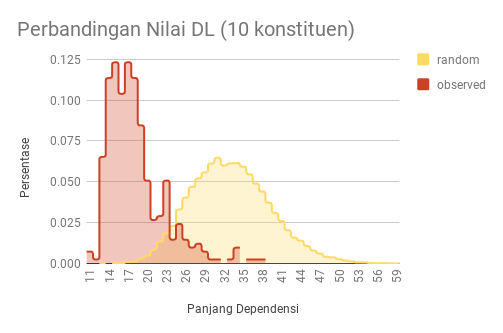
\includegraphics[width=1\linewidth]{pics/t10randomobs.png}
  \caption{10 konstituen}
  \label{fig:t10randomobs} 
\end{subfigure}
%
\begin{subfigure}{.45\textwidth}
  \centering
  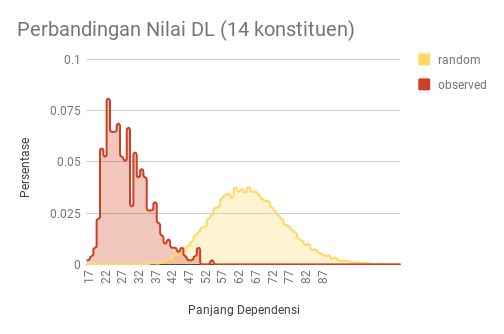
\includegraphics[width=1\linewidth]{pics/t14randomobs.png}
  \caption{14 konstituen}
  \label{fig:t14randomobs} 
\end{subfigure}
%
\begin{subfigure}{.45\textwidth}
  \centering
  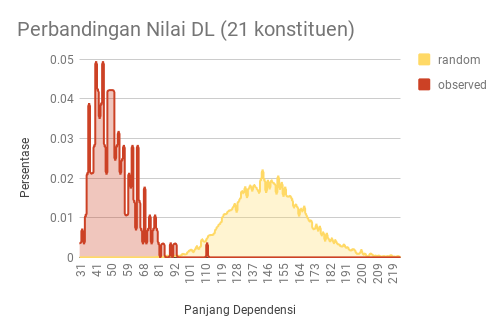
\includegraphics[width=1\linewidth]{pics/t21randomobs.png}
  \caption{21 konstituen}
  \label{fig:t21randomobs} 
\end{subfigure}

\caption{Nilai DL hasil percobaan acak dengan observasi untuk panjang kalimat 10,14, dan 21 konstituen pada data ragam tulis}
\label{fig:trandomobs}
\end{figure}


\tab~\ref{tab:perbandingan_DL_tulis} menunjukkan perbedaan rata-rata nilai DL yang cukup jauh antara hasil percobaan acak dan data observasi untuk data ragam tulis dengan efek yang signifikan pada semua jumlah konstituen (P \textless 0,001). Tes signifikansi ini dilakukan dengan menerapkan pendekatan tes Stouffer.

\begin{table}
\begin{center}
\begin{small}
  \caption{Tabel perbandingan rata-rata nilai DL hasil percobaan acak dengan data observasi dan hasil tes signifikansi untuk data ragam tulis}  \label{tab:perbandingan_DL_tulis}
  \begin{tabular}{ | l | l | l | l |}
    \hline
    	Jumlah konstituen & Rata-rata nilai DL (acak) & Rata-rata nilai DL (observasi) & p-value \\ \hline
	10 & 33,01 & 18,14 & \textless 0,001 \\ \hline
	14 & 64,95 & 29,11 & \textless 0,001 \\ \hline
	21 & 146,67 & 51,59 & \textless 0,001 \\ \hline
  \end{tabular}
  \end{small}
\end{center}
\end{table}

Sesuai dengan ekspektasi, percobaan acak terhadap data ragam lisan menunjukkan hasil yang serupa dengan percobaan terhadap data ragam tulis. \pic~\ref{fig:lrandomobs} merupakan histogram perbandingan nilai DL antara hasil percobaan acak dan data observasi untuk jumlah konstituen 5, 12, dan 22 yang mewakili setiap kelompok klasifikasi kalimat pada data ragam lisan. Histogram hasil percobaan acak untuk ragam lisan juga membentuk kurva yang secara jelas terlihat lebih rendah dan juga menandakan bahwa  acak memiliki distribusi nilai DL yang lebih besar dibandingkan dengan data observasi. Bahkan untuk jumlah konstituen 5 yang tergolong kalimat sangat pendek, data observasi masih memperlihatkan adanya indikasi DLM secara signifikan dengan nilai P \textless 0,001. Berdasarkan histogram ini juga dapat disimpulkan bahwa pada jumlah konstituen yang semakin banyak, irisan antara nilai DL data observasi dan hasil percobaan acak semakin sedikit.

\begin{figure}
\centering

\begin{subfigure}{.45\textwidth}
  \centering
  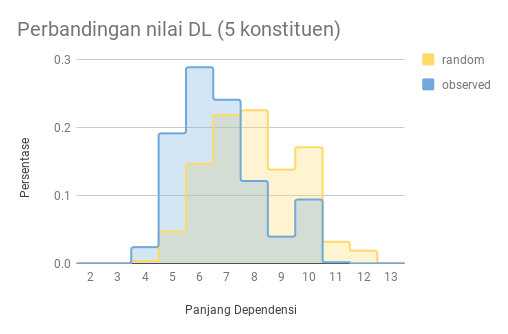
\includegraphics[width=1\linewidth]{pics/l5randomobs.png}
  \caption{5 konstituen}
  \label{fig:l5randomobs} 
\end{subfigure}
%
\begin{subfigure}{.45\textwidth}
  \centering
  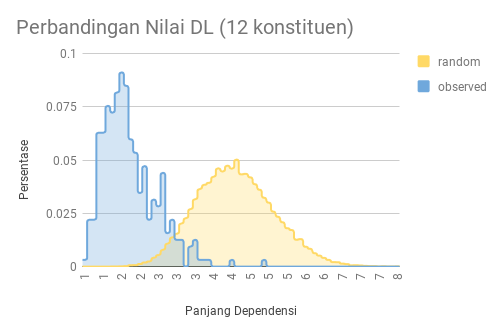
\includegraphics[width=1\linewidth]{pics/l12randomobs.png}
  \caption{12 konstituen}
  \label{fig:l12randomobs} 
\end{subfigure}
%
\begin{subfigure}{.45\textwidth}
  \centering
  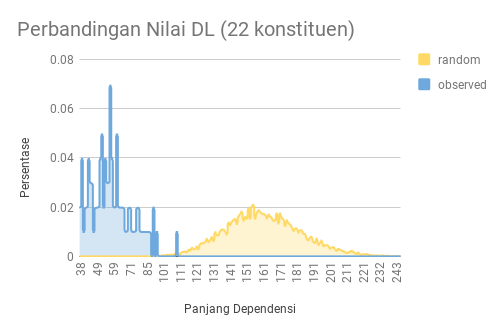
\includegraphics[width=1\linewidth]{pics/l22randomobs.png}
  \caption{22 konstituen}
  \label{fig:l22randomobs} 
\end{subfigure}

\caption{Nilai DL hasil percobaan acak dengan observasi untuk panjang kalimat 5,12, dan 22 konstituen pada data ragam lisan}
\label{fig:lrandomobs}
\end{figure}

Serupa juga dengan percobaan terhadap data ragam tulis, \tab~\ref{tab:perbandingan_DL_lisan} menunjukkan perbedaan rata-rata nilai DL yang cukup jauh antara data observasi dan hasil percobaan acak untuk data ragam lisan dengan efek yang signifikan pada semua jumlah konstituen (P \textless 0,001).

\begin{table}
\begin{center}
\begin{small}
  \caption{Tabel perbandingan rata-rata nilai DL hasil percobaan acak dengan data observasi dan hasil tes signifikansi untuk data ragam lisan}  \label{tab:perbandingan_DL_lisan}
  \begin{tabular}{ | l | l | l | l |}
    \hline
	 Jumlah konstituen & Rata-rata nilai DL (acak) & Rata-rata nilai DL (observasi) & p-value \\ \hline
	 5 & 7,98 & 6,74 & \textless 0,001 \\ \hline
	 12 & 47,7 & 24,78 & \textless 0,001 \\ \hline
	 22 & 160,89 & 58,92 & \textless 0,001 \\ \hline
  \end{tabular}
  \end{small}
\end{center}
\end{table}

Percobaan acak pada kedua korpus data dengan jumlah konstituen yang berbeda-beda menunjukkan adanya optimasi struktur ujaran pada data observasi sehingga terjadi pengurangan jarak dependensi (DLM) secara menyeluruh. Histogram hasil percobaan menunjukkan bahwa pada semua jumlah konstituen, distribusi nilai DL data observasi jauh lebih kecil mendekati jumlah minimum. Temuan ini sejalan dengan hipotesis penelitian \cite{hawkins2014cross} yang menyebutkan bahwa aturan urutan kata mendasar yang dalam pemahaman penutur akan menghasilkan konstruksi ujaran yang tautan dependensinya lebih pendek dibandingkan alternatif konstruksi yang mungkin ada.

%%-----------------------------------------------------------------------------%
\subsection{Diskusi temuan 1}
%%-----------------------------------------------------------------------------%
Hipotesis pengurangan panjang atau jarak dependensi (DLM atau DDM) berbicara tentang kecenderungan manusia untuk mendekatkan kata-kata yang memiliki relasi semantik. Pendekatan ini dapat dilakukan dengan menerapkan beberapa strategi seperti yang telah dibahas pada penelitian-penelitian terdahulu (\citealp{jaeger2006redundancy, gildea2015human}). Dalam ranah sintaksis, strategi pendekatan-kata-kata ini termasuk melalui penyusunan urutan kata dan pengurangan kata dalam kalimat (yang mungkin diakibatkan oleh pengurangan unsur yang repetitif ataupun hal yang lain). Berdasarkan tahap pertama analisis yaitu percobaan acak dengan menggunakan \textit{Free Word Order Baseline} \citep{futrell2015large} yang menghasilkan 100 kemungkinan struktur ujaran yang tidak memiliki aturan urutan kata tertentu. Percobaan ini mendukung hipotesis bahwa terjadi DLM pada kedua korpus data (ragam tulis maupun ragam lisan) secara signifikan (P \textless 0,001). 

Temuan DLM ini juga berkaitan dengan pengurangan jarak dependensi (DDM) karena percobaan acak tidak mengubah jumlah konstituen dalam ujaran yang sama sehingga variabel pembagi nilai DL sebuah ujaran tidak berubah. Temuan ini menandakan bahwa struktur ujaran-ujaran hasil observasi pada kedua ragam memperlihatkan struktur yang optimal dari segi dependensi dalam menghasilkan nilai DL yang lebih kecil dibandingkan kemungkinan struktur lain yang terbentuk. Perlu ditekankan bahwa struktur yang optimal ini dinilai dari segi dependensi dan bukan dari segi tata bahasa. Hal ini berarti terlepas dari standar gramatikal dan keberterimaannya, variasi struktur ujaran yang ada dalam kedua korpus rata-rata cukup mengoptimalkan memori kerja dan mengindikasikan kemudahan untuk berkomunikasi. Penentuan apakah sebuah struktur optimal dan juga gramatikal atau serta mudah dipahami berada di luar batasan penelitian ini. Metodologi lain seperti uji persepsi perlu dilakukan untuk mendapatkan temuan yang akurat. Penilaian dan pengukuran struktur yang lebih optimal dari segi produksi maupun pemahaman berada di luar batasan penelitian ini, sehingga perlu diadakan penelitian lebih lanjut yang melibatkan metodologi transdisipliner dengan ilmu kognitif serta uji persepsi.

%%-----------------------------------------------------------------------------%
\section{Persebaran ujaran dan kaitannya terhadap Panjang Dependensi (DL) dan Rata-rata Jarak Dependensi (MDD)}
%%-----------------------------------------------------------------------------%
Pada \pic~\ref{fig:lisantulis_DL}  dan \pic~\ref{fig:lisantulis_MDD}, terlihat jelas adanya perbedaan persebaran ujaran pada kedua korpus data terkait dengan panjang kalimat. Gambaran umum yang didapat dan garis regresi yang ditunjukkan pada kedua gambar tersebut menimbulkan pertanyaan yang hanya dapat dijawab melalui analisis dengan memperhitungkan panjang kalimatnya. Berdasarkan korpus data yang terkumpul, persebaran ujaran pada kedua ragam berbeda secara signifikan. Pad data ragam tulis, sebanyak 45,54\% ujaran berada pada klasifikasi kalimat menengah (\tab~\ref{tab:presentase_ujaran}). Klasifikasi kalimat pendek dan panjang pada ragam tulis memiliki jumlah ujaran yang tidak jauh berbeda. Sedangkan, sebanyak 59,49\% ujaran pada data ragam lisan berada pada klasifikasi kalimat pendek dan menurun secara drastis pada klasifikasi kalimat menengah dan panjang.

\begin{table}
\begin{center}
\begin{small}
   \caption{Persentase ujaran pada tabel klasifikasi jumlah konstituen}  \label{tab:presentase_ujaran}
  \begin{tabular}{ |p{3cm} | p{3cm} | p{3cm} | p{3cm} |}
    \hline
 & Kalimat Pendek \newline (\textless=10 konstituen) & Kalimat Menengah (11-20 konstituen) & Kalimat Panjang (\textgreater20 konstituen) \\ \hline
Data Ragam Tulis & 23,33\% & 45,54\% & 31,13\% \\ \hline
Data Ragam Lisan & 59,49\% & 29,16\% & 11,35\% \\ \hline
  \end{tabular}
  \end{small}
\end{center}
\end{table}


Pada \pic~\ref{fig:jumlah_kata}, dapat dilihat adanya pergeseran diagram persebaran ujaran berdasarkan panjang kalimat. Ujaran dengan frekuensi terbanyak pada data ragam tulis adalah ujaran dengan ujaran dengan panjang kalimat sebanyak 14 konstituen. Sedangkan pada ragam lisan, frekuensi terbanyak ditemukan pada ujaran dengan panjang kalimat sebanyak 5 konstituen. 

\begin{figure}
	\centering 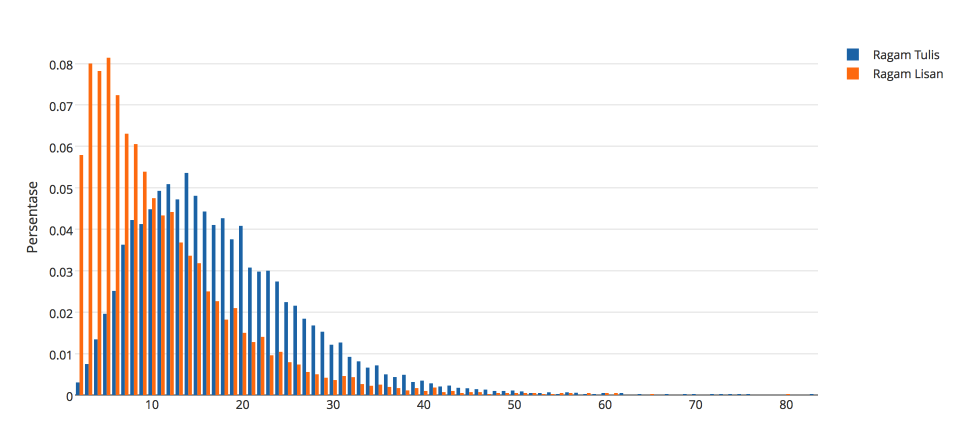
\includegraphics[width=1
	\textwidth] {pics/Jumlah_kata.png} 
	\caption{Diagram perbandingan jumlah konstituen data ragam lisan dan tulis} 
	\label{fig:jumlah_kata} 
\end{figure}

%%-----------------------------------------------------------------------------%
\section{Temuan 2: Pemusatan data ragam lisan pada klasifikasi kalimat pendek (\textless= 10 konstituen)}
%%-----------------------------------------------------------------------------%
Pemusatan data pada klasifikasi kalimat pendek (\textless= 10 konstituen) pada data ragam lisan cukup besar hingga melebihi 50\% dari total jumlah kalimat dalam korpus tersebut. Hal ini berdampak pada perbandingan rata-rata nilai DL serta MDD antara data ragam tulis dan lisan pada kelompok klasifikasi tersebut (\tab~\ref{tab:DL_MDD_pendek}).

\begin{table}
\begin{center}
\begin{small}
\caption{Perbandingan rata-rata nilai DL dan MDD pada klasifikasi kalimat pendek }\label{tab:DL_MDD_pendek}
  \begin{tabular}{ | p{3.2cm} | p{3.2cm} | p{3.2cm} | p{2cm} |}
    \hline
 & Kalimat Pendek \newline (\textless =10 konstituen) \newline Data Ragam Tulis & Kalimat Pendek \newline (\textless =10 konstituen) \newline Data Ragam Lisan & \textit{p-value} \\ \hline
 Rata-rata Nilai DL & 11,85 & \textbf{8,76} & \textless 0,001 \\ \hline
 Rata-rata Nilai MDD & 1,792 & \textbf{1,687} & \textless 0,001 \\ \hline
 Rata-rata Jumlah Konstituen & 7,356 & \textbf{5,708} & \textless 0,001 \\ \hline
 Jumlah Ujaran & 2220 & 6073 & -- \\ \hline
   \end{tabular}
   \end{small}
\end{center}
\end{table}


Berdasarkan \tab~\ref{tab:perbandingan_DL_MDD}, Nilai DL dan MDD data ragam lisan lebih kecil dibandingkan data ragam tulis pada klasifikasi kalimat pendek secara signifikan. Berbeda dengan \pic~\ref{fig:lisantulis_DL}  dan \pic~\ref{fig:lisantulis_MDD} yang tidak memperhitungkan klasifikasi panjang kalimat, terutama pada nilai DL yang bersifat cukup linier terhadap panjang kalimat, rata-rata nilai DL pada data ragam lisan pada klasifikasi ini adalah 8,76. Nilai ini lebih rendah dibandingkan dengan nilai yang didapatkan dari data ragam tulis karena pemusatan jumlah konstituen yang mendekati minimum pada data ragam lisan akan mempengaruhi hasil yang didapat. Hal ini dapat dilihat dari perbandingan rata-rata jumlah konstituen dan jumlah ujaran yang muncul pada klasifikasi ini dengan perbedaan yang signifikan. Meskipun jumlah ujaran data ragam lisan pada klasifikasi ini jauh lebih banyak, rata-rata jumlah konstituen dalam satu ujaran lebih sedikit dibandingkan data ragam tulis.  Berkaitan dengan pemusatan data tersebut, rata-rata nilai MDD data ragam lisan juga menjadi lebih kecil dibandingkan data ragam tulis. Temuaan ini memberikan indikasi bahwa penggunaan kalimat pendek menjadi salah satu preferensi (dan mungkin strategi)  untuk meningkatkan efisiensi ujaran dalam percakapan lisan. Dalam beberapa kasus di korpus data ragam lisan, ditemukan ujaran-ujaran yang sebenarnya merupakan klausa terikat yang berdiri sendiri sebagai sebuah ujaran utuh dan lepas dari klausa pada ujaran sebelumnya. Seperti contoh, ujaran-ujaran ini banyak ditemukan ditandai dengan konjungsi 'dan' pada posisi pertama dalam ujaran. 

%%-----------------------------------------------------------------------------%
\subsection{Temuan 3: Perbandingan terbalik antara Panjang Dependensi (DL) dan Rata-rata Jarak Dependensi (MDD) pada klasifikasi kalimat menengah (11-20 konstituen)}
%%-----------------------------------------------------------------------------%
Pada kelompok klasifikasi kalimat menengah dengan panjang kalimat sebanyak 11 hingga 20 konstituen, terlihat adanya perbedaan dalam perbandingan nilai-nilai antara kedua ragam. Pada klasifikasi ini ditemukan perbandingan terbalik antara rata-rata nilai DL dan MDD pada kedua korpus data (\tab~\ref{tab:DL_MDD_menengah}). Untuk nilai DL, data ragam lisan memiliki rata-rata yang sedikit lebih rendah, yaitu 33,05 dibandingkan data ragam tulis (33,32) namun perbedaan ini tidak signifikan (\textit{P} \textgreater 0,05). Hal ini berarti pemusatan ujaran ragam lisan yang banyak mendekati kalimat pendek atau persebaran ujaran ragam tulis di kelompok klasifikasi ini yang cukup merata mungkin tidak mempengaruhi nilai tersebut. Meskipun begitu, temuan yang menarik adalah bahwa rata-rata nilai MDD data ragam tulis (2,31) lebih rendah dibandingkan dengan data ragam lisan (2,41) secara signifikan. Jumlah ujaran kedua korpus data tidak jauh berbeda dan selisih rata-rata jumlah konstituen juga tidak sebesar pada klasifikasi kalimat pendek namun perbedaannya signifikan. Hal ini berarti pada klasifikasi kalimat menengah, masih terlihat kecenderungan untuk menggunakan ujaran yang lebih pendek pada ragam lisan.  

\begin{table}
\begin{center}
\begin{small}
\label{table:DL_MDD_menengah}
 \caption{Perbandingan rata-rata nilai DL dan MDD pada klasifikasi kalimat menengah}  \begin{tabular}{| p{3.2cm} | p{3.2cm} | p{3.2cm} | p{2cm} |}
    \hline
 & Kalimat Menengah \newline (11-20 konstituen) \newline Data Ragam Tulis & Kalimat Menengah \newline (11-20 konstituen) \newline Data Ragam Lisan & \textit{p-value} \\ \hline
 Rata-rata Nilai DL & 33,32 & 33,05 & \textgreater 0,05  \\ \hline
 Rata-rata Nilai MDD & \textbf{2,31} & 2,41 & \textless 0,001 \\ \hline
 Rata-rata Jumlah Konstituen & 15,24 & \textbf{14,56} & \textless 0,001 \\ \hline
 Jumlah Ujaran & 4210 & 2976 & -- \\ \hline
   \end{tabular}
   \end{small}
\end{center}
\end{table}


Rata-rata nilai DL dan MDD kedua korpus data yang berbanding terbalik menunjukkan adanya indikasi bahwa pada panjang kalimat tertentu, jumlah konstituen yang lebih sedikit tidak selalu berfungsi sebagai strategi untuk menghasilkan kalimat yang efisien dari segi dependensi. Indikasi pada kelompok klasifikasi ini menarik karena memperlihatkan bahwa meskipun jumlah nilai yang dihasilkan semua tautan dependensi lebih kecil, tidak berarti menggambarkan jarak antarkonstituen yang lebih kecil juga.

%%-----------------------------------------------------------------------------%
\subsection{Temuan 4: Tidak ada kecenderungan jumlah konstituen pada klasifikasi kalimat panjang (\textgreater20 konstituen)}
%%-----------------------------------------------------------------------------%

Berbeda dengan kedua klasifikasi panjang kalimat sebelumnya, rata-rata nilai DL dan MDD pada data ragam tulis lebih kecil dibandingkan data ragam lisan (\tab~\ref{tab:DL_MDD_panjang}) dan perbedaan ini bersifat signifikan. Hal ini berarti terlepas dari persebaran ujarannya yang cukup banyak (31,13\%) dari keseluruhan korpus data ragam tulis), ujaran dengan jumlah konstituen yang lebih banyak data ragam tulis cenderung memiliki struktur yang lebih efisien dibandingkan dengan data ragam lisan. Pada kelompok klasifikasi menengah, nilai MDD data ragam tulis lebih kecil dibandingkan data ragam lisan secara signifikan. Temuan tersebut dan temuan pada klasifikasi ini menunjukkan bahwa mulai panjang kalimat tertentu, meskipun kompleksitas kalimat semakin tinggi (nilai DL makin tinggi), data ragam tulis menunjukkan struktur yang menyebabkan tautan antarkonstituen lebih pendek sehingga mendukung efisiensi ujaran. Jumlah ujaran antara keduanya cukup jauh berbeda, tetapi selisih rata-rata jumlah konstituen sangat kecil dan perbedaannya tidak signifikan. Hal ini berarti pada klasifikasi kalimat panjang berdasarkan data yang dikumpulkan, tidak ada kecenderungan atau preferensi terkait panjang kalimat pada kedua ragam. 

\begin{table}
\caption{Perbandingan rata-rata nilai DL dan MDD pada klasifikasi kalimat panjang}  \label{table:DL_MDD_panjang}
\begin{center}
\begin{small}
\begin{tabular}{ | p{3.2cm} | p{3.2cm} | p{3.2cm} | p{2cm} |}
    \hline
 & Kalimat Panjang \newline (\textgreater20 konstituen) \newline Data Ragam Tulis & Kalimat Panjang \newline (\textgreater20 konstituen) \newline Data Ragam Lisan & \textit{p-value} \\ \hline
 Rata-rata Nilai DL & \textbf{79,94} & 83,84 & \textless 0,01 \\ \hline
 Rata-rata Nilai MDD & \textbf{2,844} & 3,018 & \textless 0,001 \\ \hline
 Rata-rata Jumlah Konstituen & 28,39 & 28,36 & \textgreater 0,05 \\ \hline
 Jumlah Ujaran & 2876 & 1158 & -- \\ \hline
   \end{tabular}
   \end{small}
\end{center}
\end{table}

Untuk memberikan ilustrasi terhadap perbandingan struktur ujaran kelompok klasifikasi kalimat panjang, berikut adalah beberapa contoh ujaran dengan jumlah konstituen sebanyak 31 yang diambil dari kedua korpus data (\pic~\ref{fig:ts2079}, \pic~\ref{fig:ts2081}, \pic~\ref{fig:ls1716}, \pic~\ref{fig:ls16}, dan \pic~\ref{fig:ls114}). Kelima ujaran tersebut menunjukkan adanya karakter utama yang secara cukup jelas membedakan karakteristik struktur ujaran pada data ragam tulis dan lisan. Kata 'penting' pada ujaran T31a (\pic~\ref{fig:ts2079}) dan 'ditingkatkan' pada ujaran T31b (\pic~\ref{fig:ts2081}) sama-sama merupakan akar yang memiliki beberapa tautan dependensi terhadap konstituen terikatnya. Kesamaan kedua iujaran pada ragam tulis ini adalah bahwa induk pada simpai cabang terdekat yang diikat oleh akar cenderung memiliki jumlah konstituen sedikit meskipun mengandung beberapa klausa terikat. Pola ini terlihat berulang pada simpai-simpai cabang berikutnya. Struktur ujaran dengan karakteristik seperti pada \pic~\ref{fig:ts2079} dan \pic~\ref{fig:ts2081} ini cukup umum dalam korpus data ragam tulis klasifikasi kalimat panjang.

Pada ujaran T31a (\pic~\ref{fig:ts2079}), akar adjektiva 'penting' mengikat verba 'memperbaiki' yang dihubungkan dengan konjungsi tujuan 'untuk' dalam kaidah dependensi. Sedangkan pada ujaran T31b (\pic~\ref{fig:ts2081}), akar verbal 'ditingkatkan' mengikat verba lain 'mempercepat' yang juga dihubungkan dengan konjungsi tujuan 'untuk'. Pada kedua ujaran dalam ragam tulis, simpai-simpai selanjutnya tidak memiliki tautan langsung dengan akar, melainkan memiliki relasi antarsimpai yang bersifat berlanjut, mencerminkan percabangan searah. Relasi ini membentuk lapisan level dependensi yang semakin mendalam secara bertahap. Dalam diagram pohon kedua ujaran, relasi ini terlihat melalui pergerakan simpai dan percabangan yang semakin menurun ke arah sesudah akar atau ke arah kanan. Percabangan menurun ke kanan ini juga menunjukkan indikasi adanya strategi untuk menghasilkan dependensi positif (konstituen terikat sesudah induk) dan relasi antarkonstituen utama yang bersifat \textit{head-initial}. Hal ini berarti untuk percabangan setelah akar dapat langsung diproses oleh kognisi manusia karena akar (yang merupakan konstituen dengan kandungan informasi utama) sudah direalisasikan terlebih dahulu (\citeal{tesniere1959elements, wang2017effects}). Ujaran T31a (\pic~\ref{fig:ts2079}) memiliki nilai DL sebesar 56 dan nilai MDD sebesar 1,867, sedangkan ujaran T31b (\pic~\ref{fig:ts2081}) memiliki nilai DL 67 dan nilai MDD 2,233.

\begin{figure}
	\centering 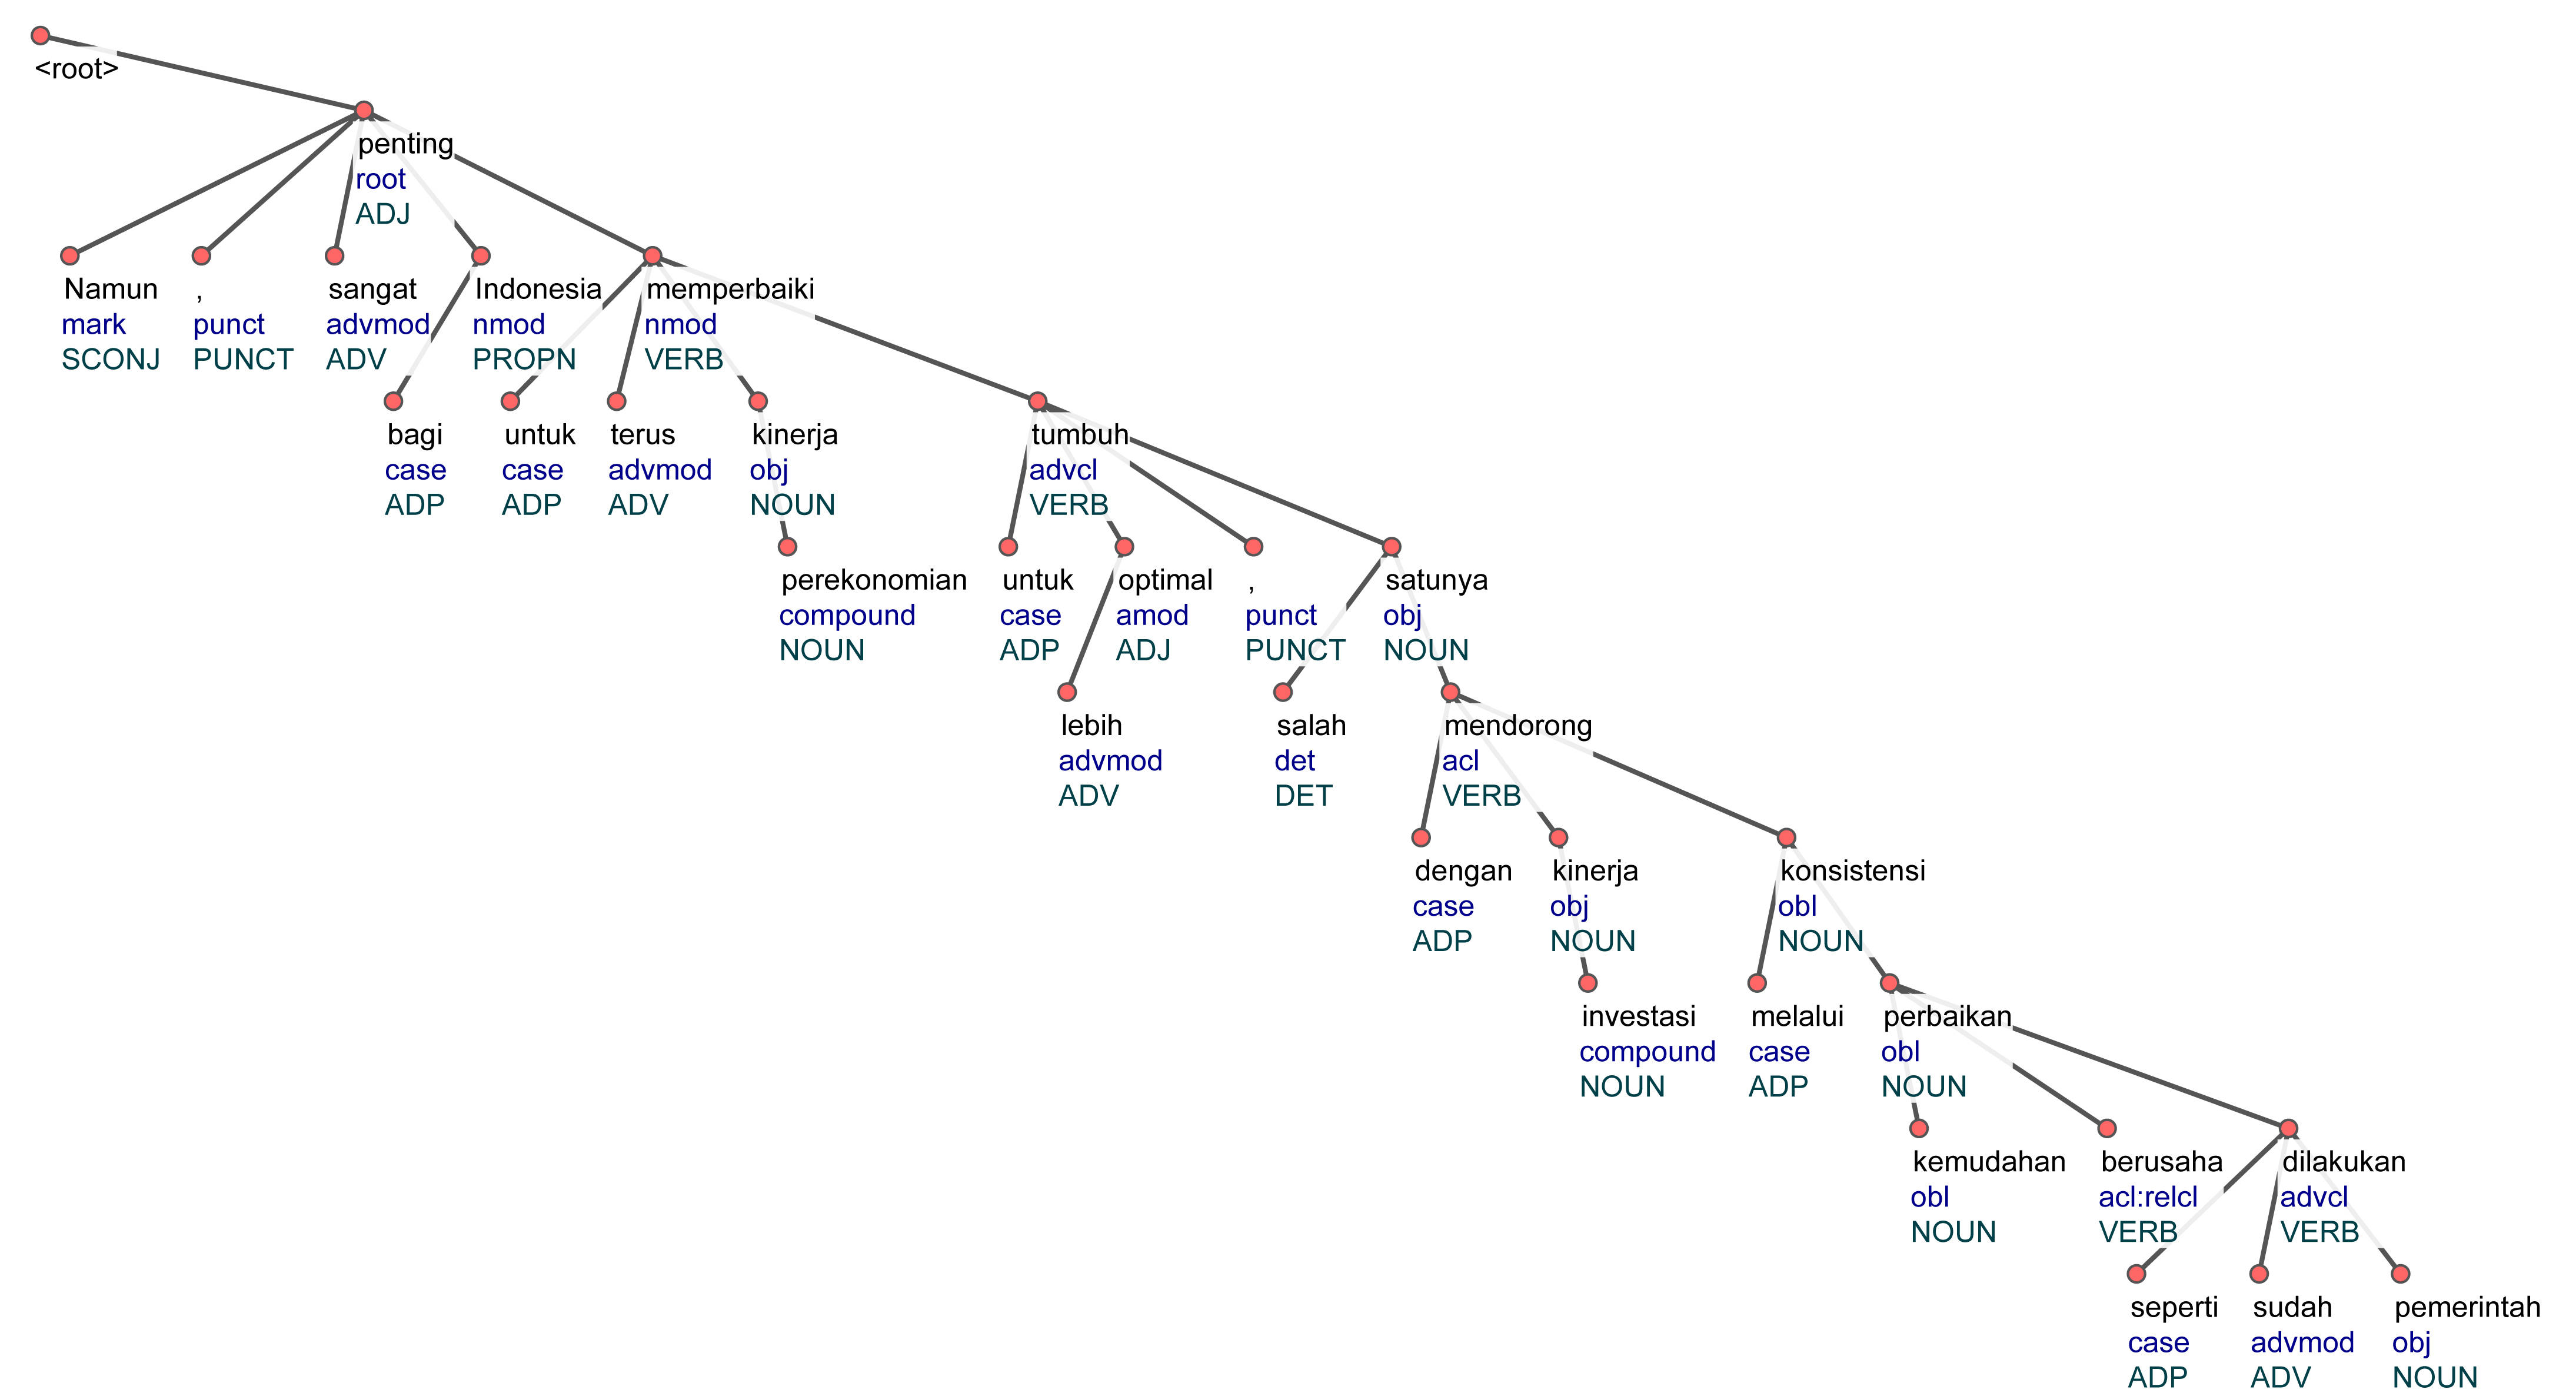
\includegraphics[width=1
	\textwidth] {pics/ts2079.jpg} 
	\caption{Ujaran T31a pada data ragam tulis} 
	\label{fig:ts2079} 
\end{figure}

\begin{figure}
	\centering 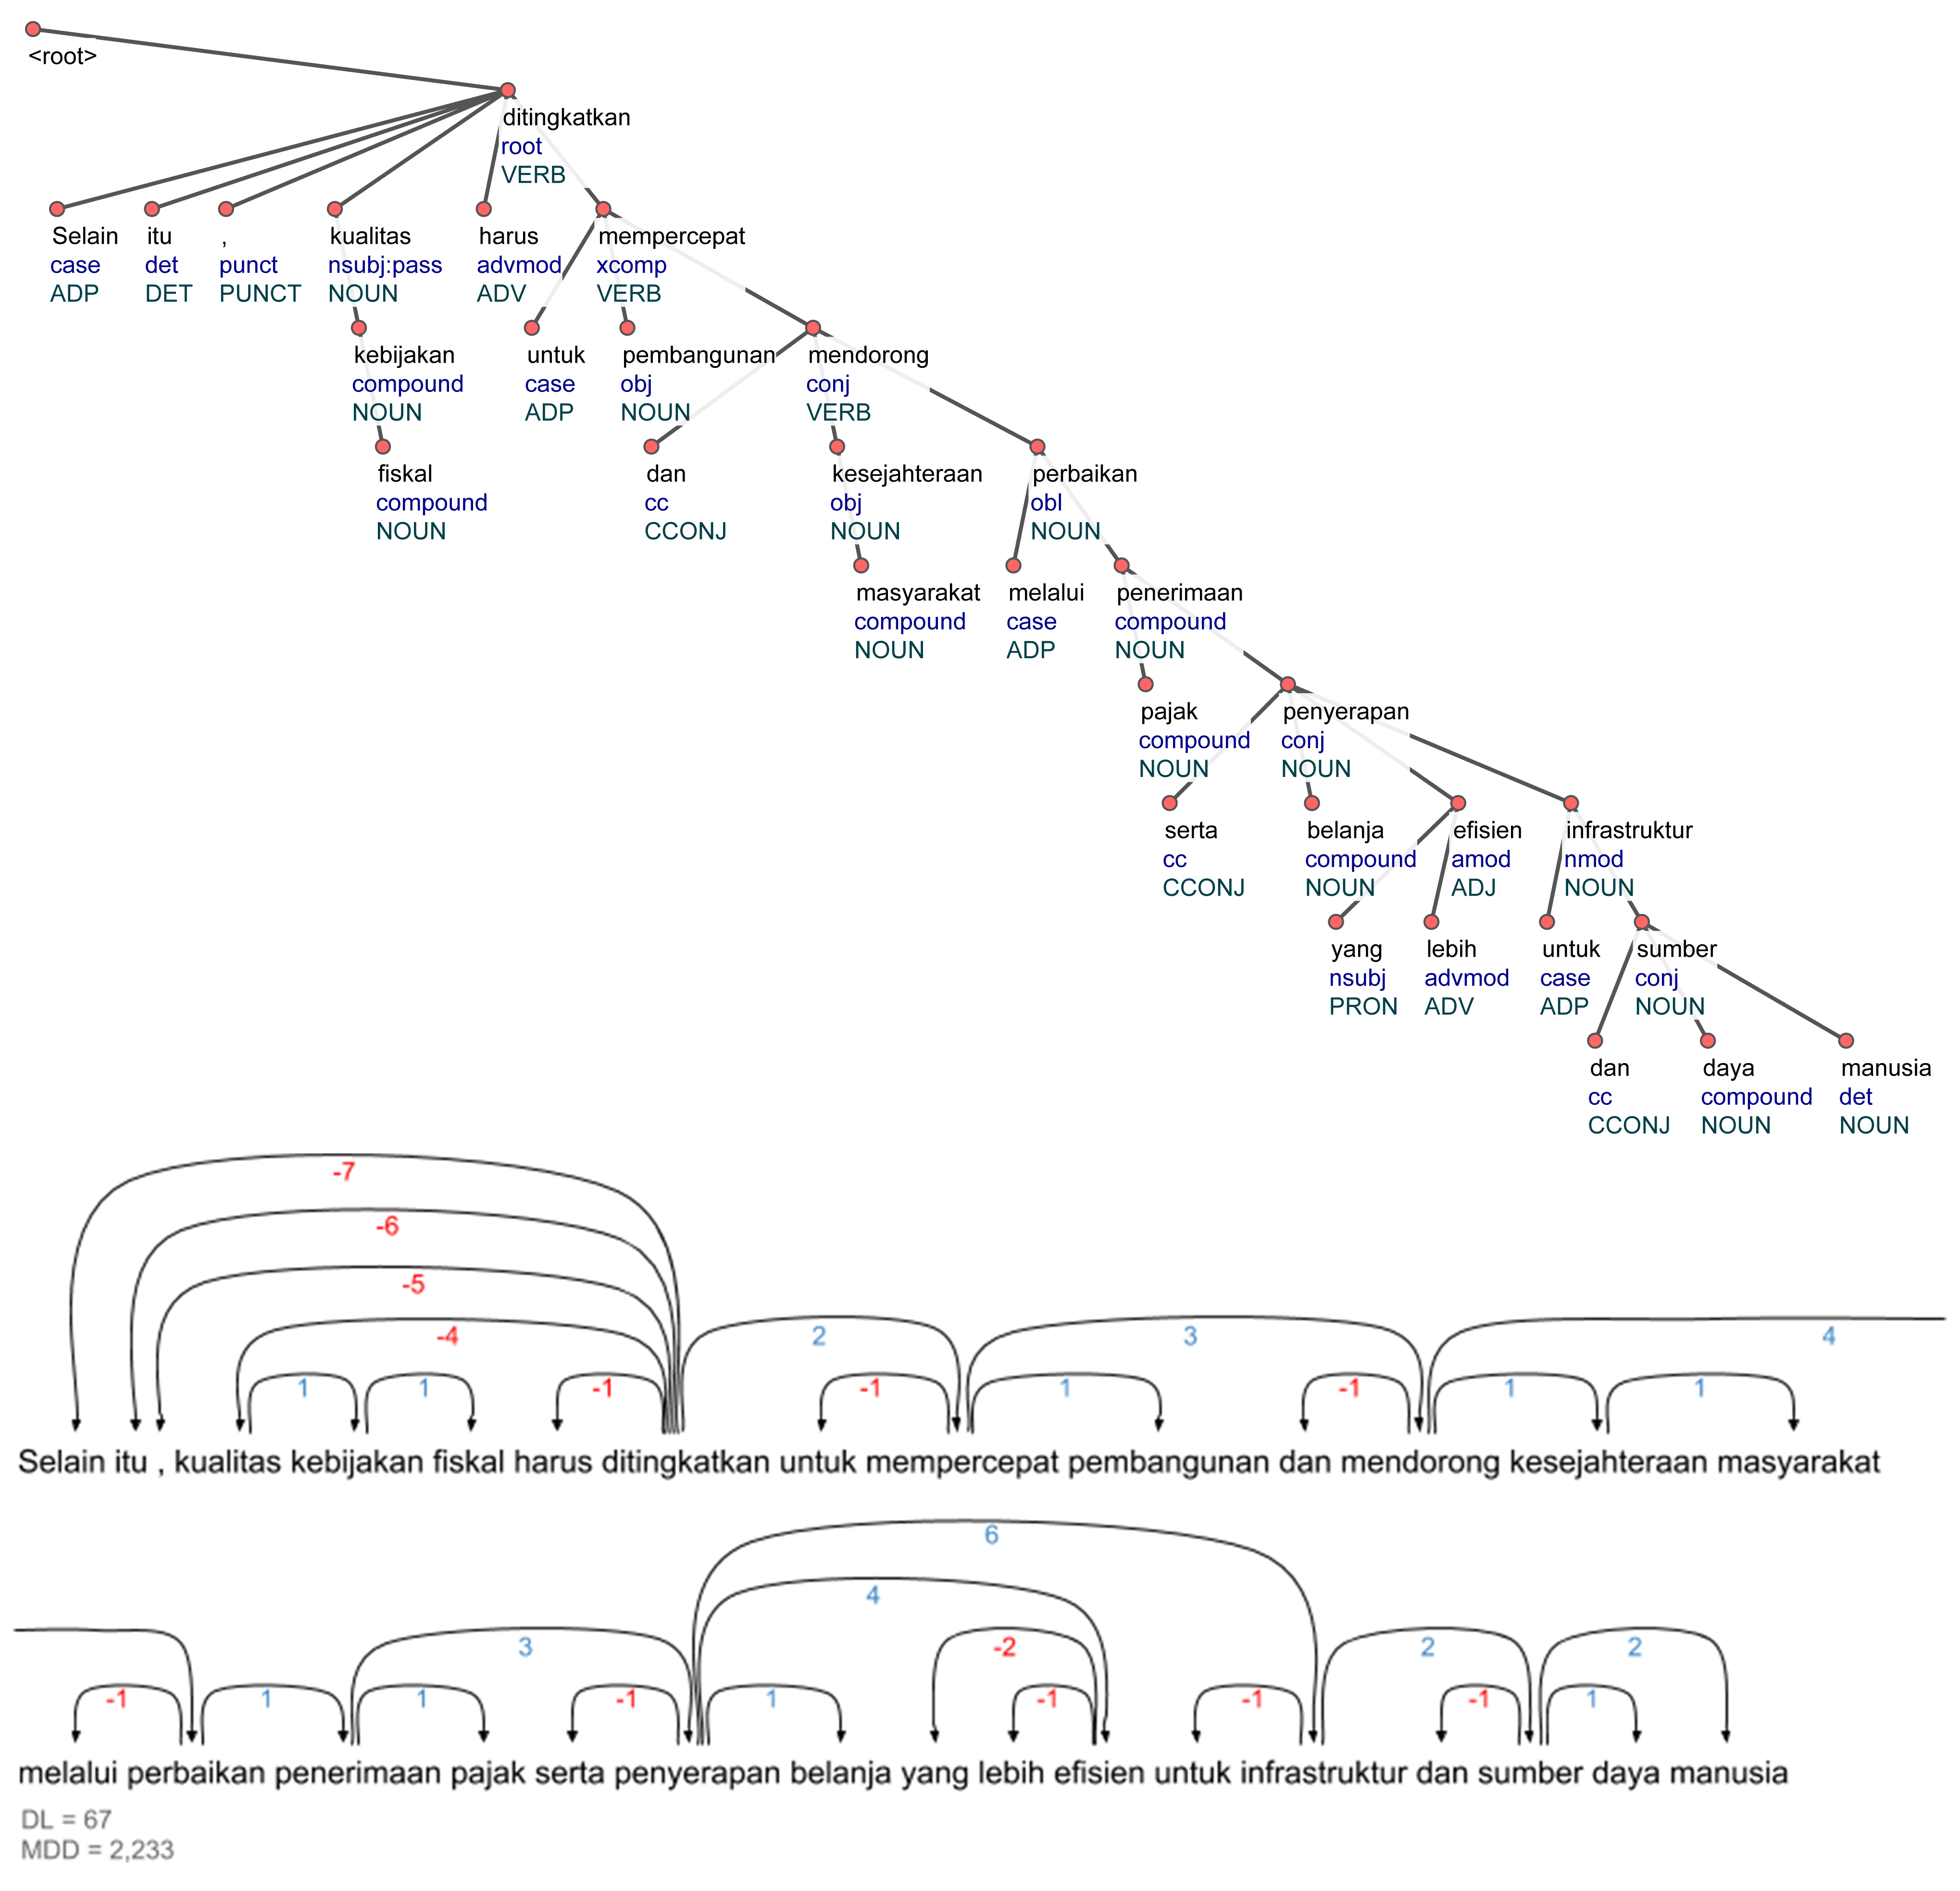
\includegraphics[width=1
	\textwidth] {pics/ts2081.jpg} 
	\caption{Ujaran T31b pada data ragam tulis} 
	\label{fig:ts2081} 
\end{figure}

Ujaran L31a (\pic~\ref{fig:ls1716}), L31b (\pic~\ref{fig:ls16}), dan L31c(\pic~\ref{fig:ls114}) sedikit berbeda satu sama lain namun memiliki karakter utama yang serupa yang membedakannya dengan \pic~\ref{fig:ts2079} dan \pic~\ref{fig:ts2081} pada data ragam tulis. Salah satunya adalah perbedaan posisi akar pada \pic~\ref{fig:ls1716}, \pic~\ref{fig:ls16}, dan \pic~\ref{fig:ls114}. Pada ujaran L31a (\pic~\ref{fig:ls1716}), simpai pusat dan simpai cabang pada verba 'dipaksa' memiliki banyak tautan yang cukup seimbang. Ujaran ini memperlihatkan adanya pembagian informasi secara besar. Relasi akar verbal 'berdatangan' dengan verba 'dipaksa' memiliki tipe dependensi $parataxis$. Tipe ini menandakan relasi yang menyerupai koordinasi antar diskursus, dalam arti seluruh informasi yang dibawa oleh simpai konstituen terikat ini bisa menjadi ujaran terpisah. Pada ujaran L31b (\pic~\ref{fig:ls16}), seluruh informasi yang dibawa klausa tujuan dengan induk 'memastikan' direalisasikan sebelum akar verbal 'menanyakan'. Akar verbal ini juga mengikat verba 'dibantah' yang dihubungkan dengan konjungsi 'dan'. Pada ujaran tersebut, akan berada di tengah kalimat dan pembagian informasi juga cukup merata. Ujaran L31c (\pic~\ref{fig:ls114}) memiliki akar cenderung di posisi akhir. Beberapa simpai dan informasi yang dibawa oleh simpai tersebut harus direalisasikan dulu sebelum akar verbal 'kira'. Di bawah simpai 'Pak', terlihat adanya indikasi percabangan searah, yaitu relasi antara 'Pak' dengan 'melakukan' dan 'melakukan' dengan 'peresmian'. Namun seluruh relasi ini berada di bawah tautan utama antara 'kira' dengan 'Pak', sehingga terjadi percabangan yang bersifat kombinasi antara searah dan beda arah. Ujaran L31a (\pic~\ref{fig:ls1716}) memiliki nilai DL sebesar 86 dan nilai MDD sebesar 2,867, ujaran L31b (\pic~\ref{fig:ls16}) memiliki nilai DL 67 dan nilai MDD 2,233, dan L31c(\pic~\ref{fig:ls114}) memiliki nilai DL 89 dan nilai MDD 2,967.

\begin{figure}
	\centering 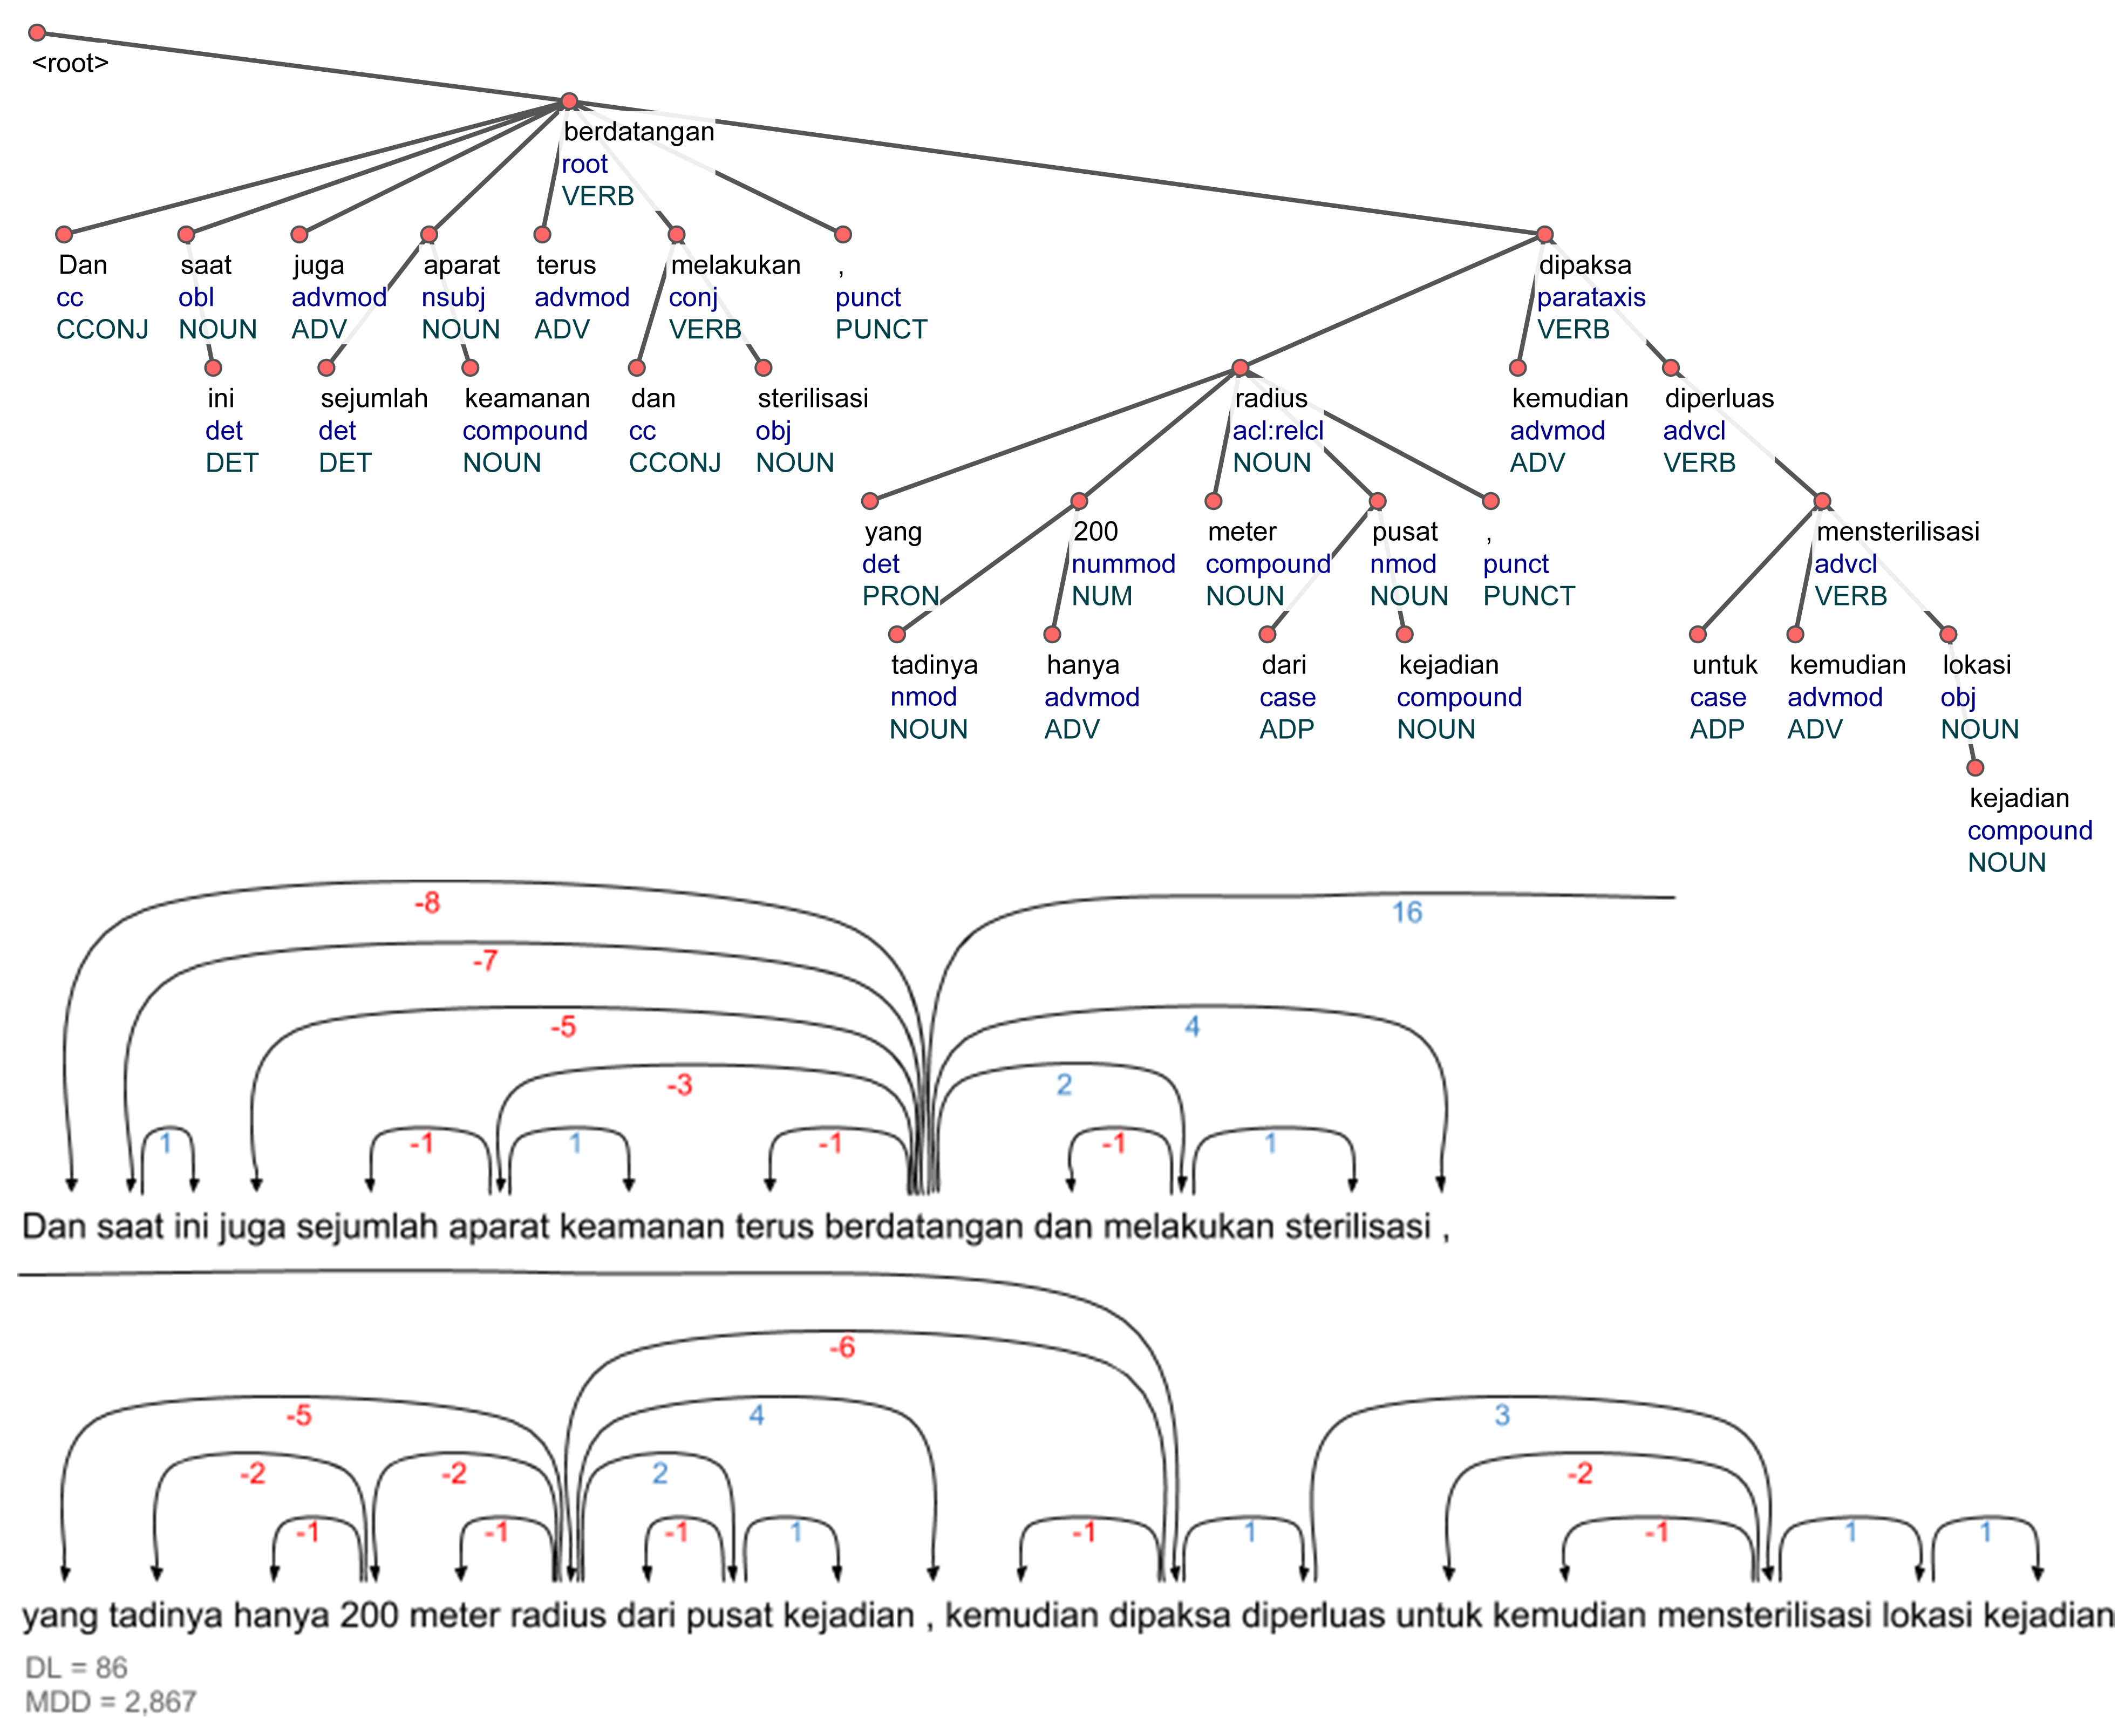
\includegraphics[width=1
	\textwidth] {pics/ls1716.jpg} 
	\caption{Ujaran L31a pada data ragam lisan} 
	\label{fig:ls1716} 
\end{figure}

\begin{figure}
	\centering 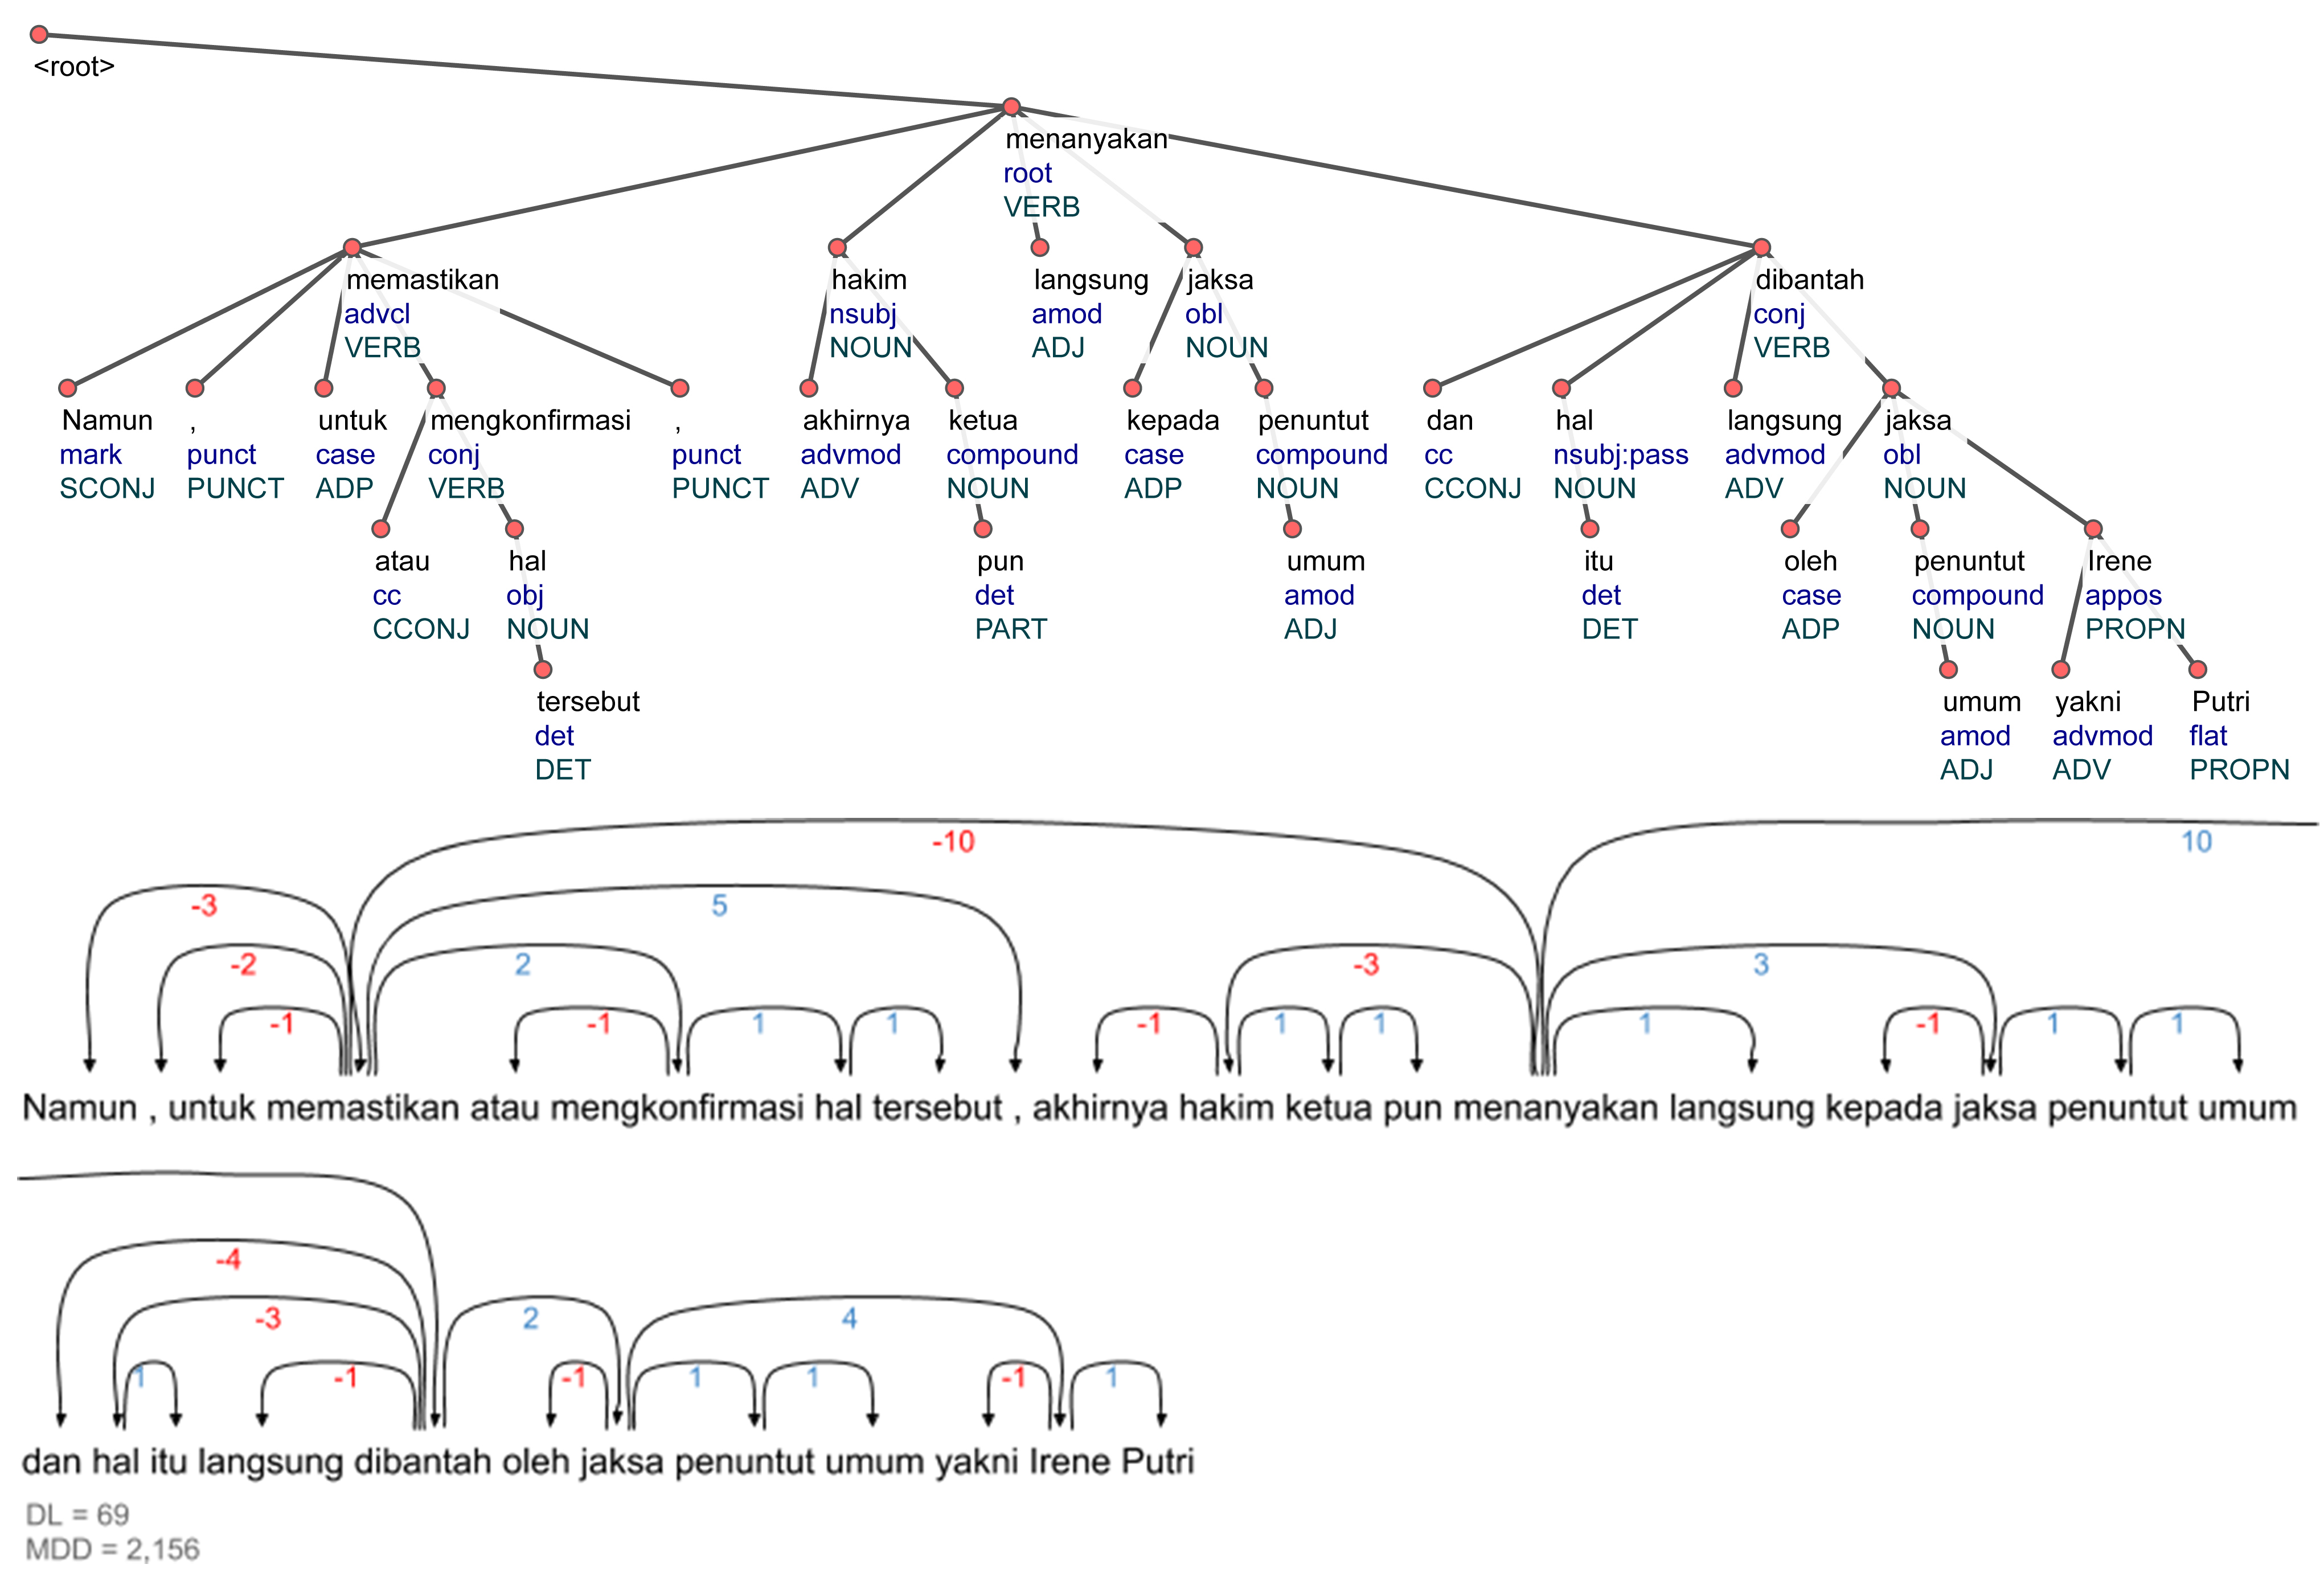
\includegraphics[width=1
	\textwidth] {pics/ls16.jpg} 
	\caption{Ujaran L31b pada data ragam lisan}
	\label{fig:ls16} 
\end{figure}

\begin{figure}
	\centering 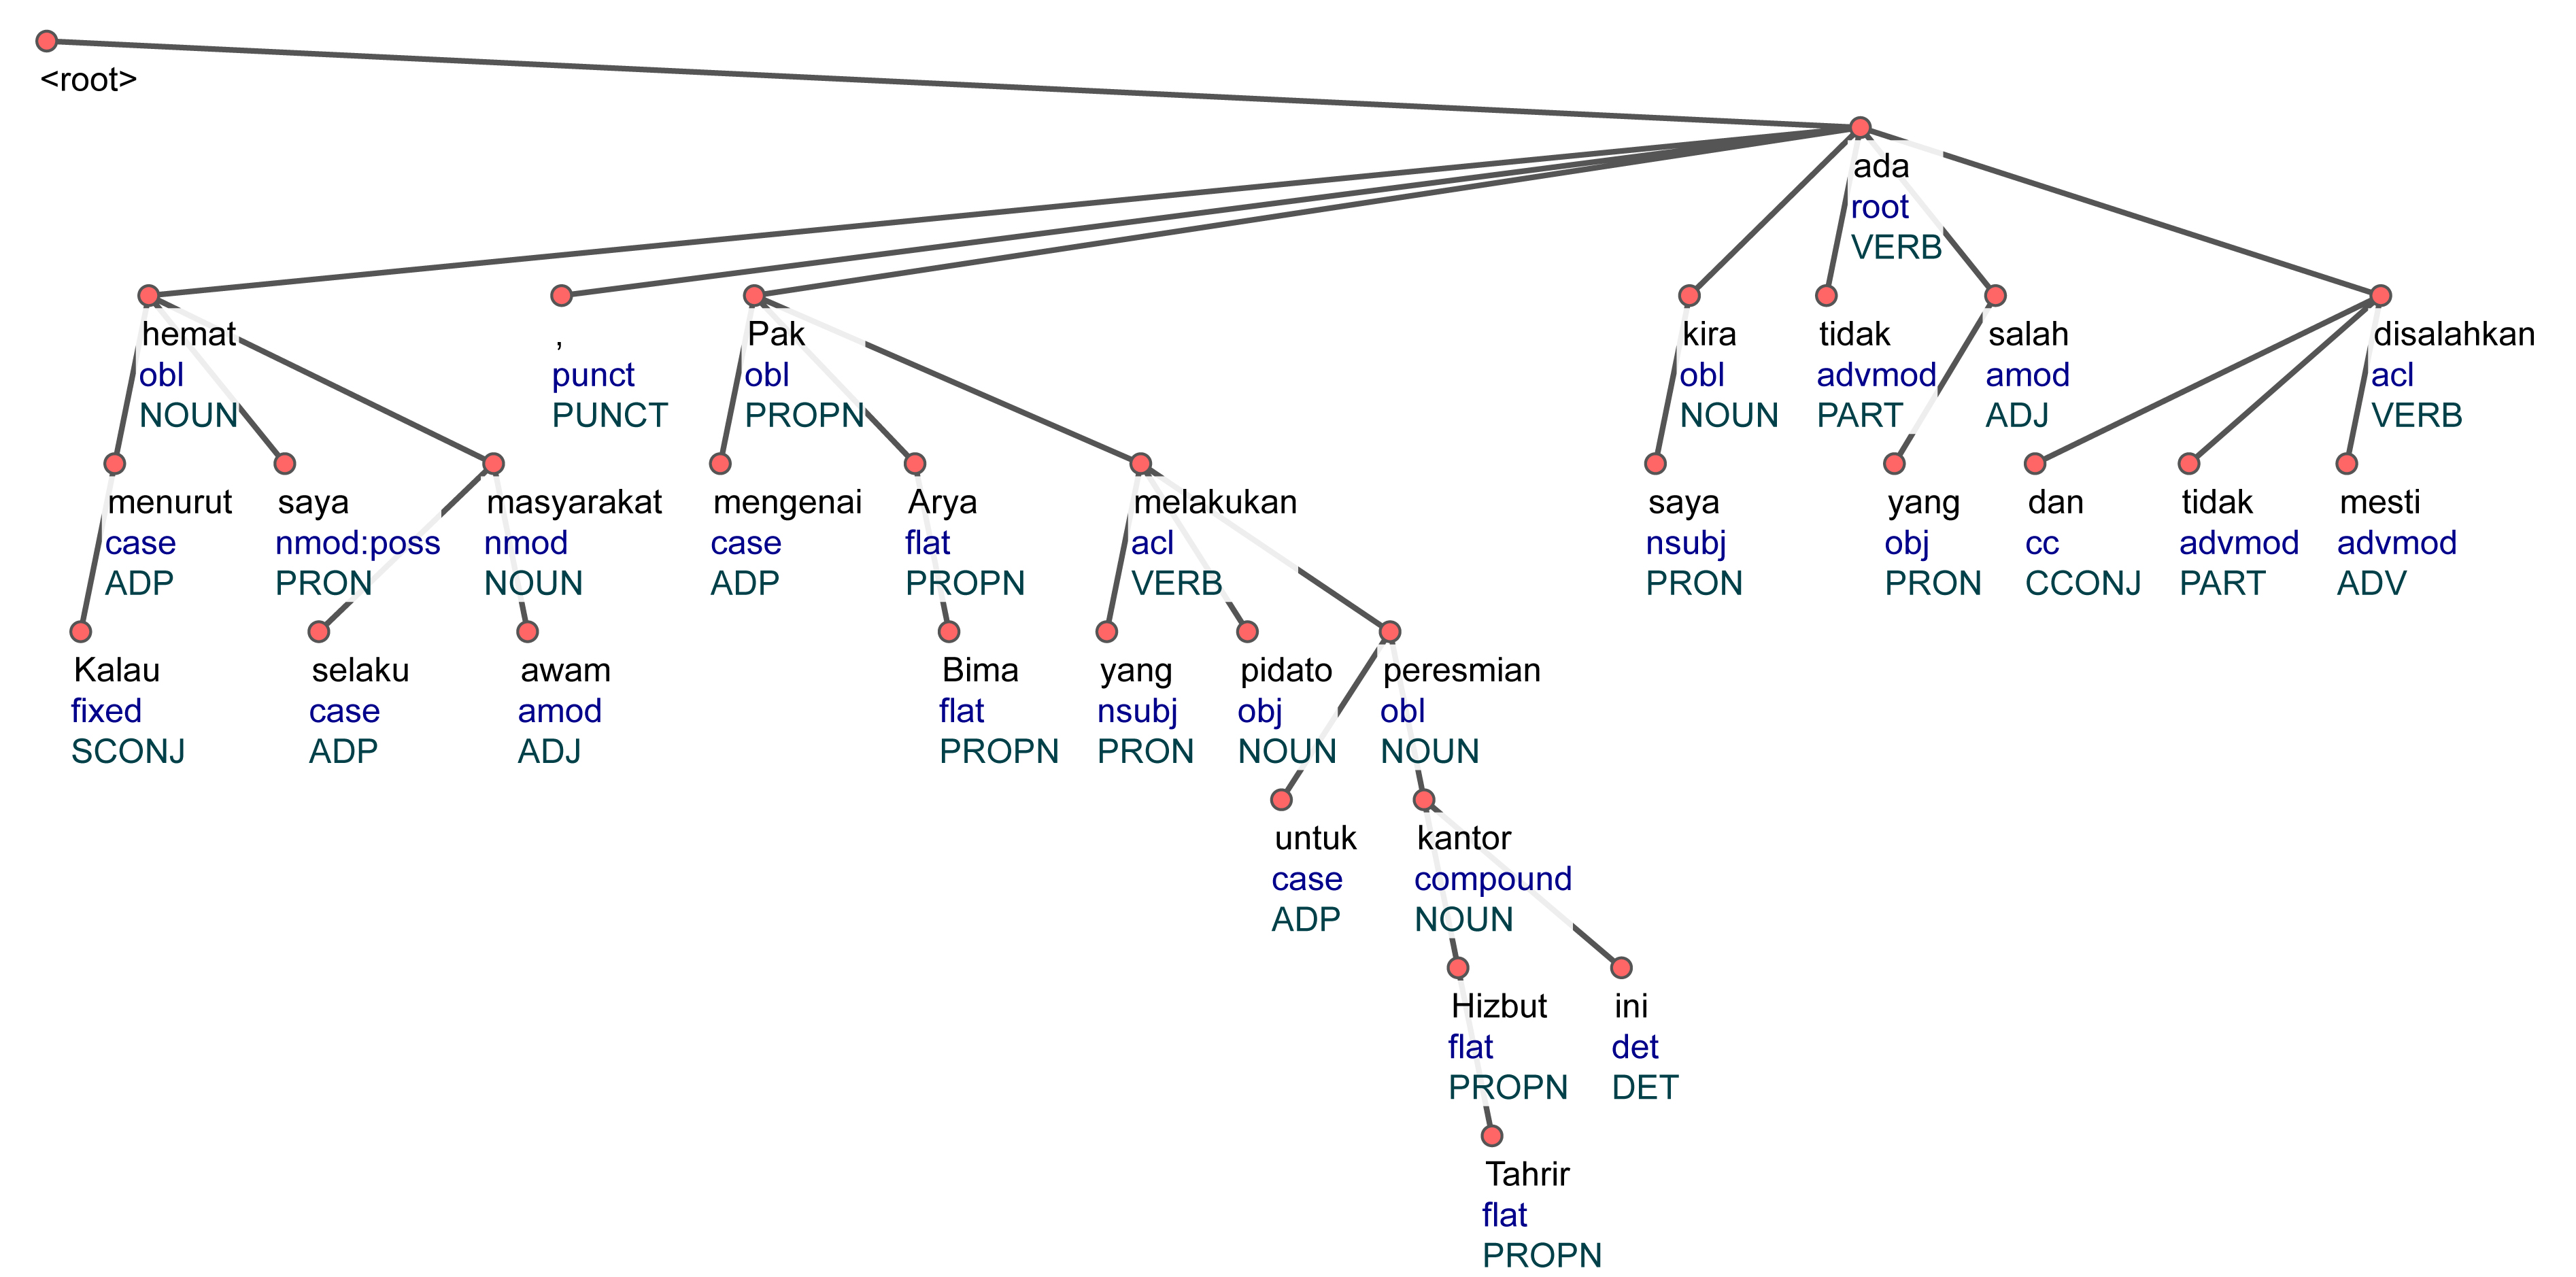
\includegraphics[width=1
	\textwidth] {pics/ls114.jpg} 
	\caption{Ujaran L31c pada data ragam lisan}
	\label{fig:ls114} 
\end{figure}

Berdasarkan diagram-diagram pohon tersebut, perbedaan yang paling terlihat antara contoh-contoh pada ragam lisan dibandingkan dengan contoh-contoh pada ragam tulis adalah percabangannya yang terlihat lebih tidak konsisten. Meskipun tidak semua ujaran memiliki struktur seperti \pic~\ref{fig:ts2079} dan \pic~\ref{fig:ts2081}, mayoritas ujaran kalimat panjang pada data ragam tulis menunjukkan karakter yang lebih konsisten dalam hal pergerakan percabangannya. Pada data ragam lisan, terlihat banyak kombinasi antara percabangan searah dan beda arah serta letak posisi akar yang menyebar dari awal hingga akhir ujaran. Percabangan utama yang tersebar pada ketiga ujaran tersebut menunjukkan indikasi hubungan klausa yang tidak bersifat berlanjut, namun paralel. Ujaran L31b (\pic~\ref{fig:ls16}) dan L31c (\pic~\ref{fig:ls114}) memiliki percabangan utama sebelum akar sehingga secara kolektif membentuk relasi dependensi utama yang negatif. Hal ini berarti seluruh informasi yang dibawa oleh klausa-klausa pada simpai dan percabangan sebelum akar harus disimpan dalam memori kerja dan menunggu realisasi akar agar penggalan informasi yang dibawa simpai tersebut dapat diproses secara utuh oleh kognisi manusia \citep{hawkins2014cross}.

%%-----------------------------------------------------------------------------%
\section{Diskusi temuan 2, 3, dan 4}
%%-----------------------------------------------------------------------------%
Berdasarkan percobaan acak yang dilakukan, langkah analisis selanjutnya adalah melihat aspek-aspek yang mungkin mempengaruhi struktur ujaran sehingga memungkinkan terjadinya DLM dan DDM. Secara garis besar, analisis-analisis lanjutan untuk melihat aspek-aspek ini menghasilkan temuan strategi yang berkaitan dengan panjang kalimat, pengaturan urutan kata terkait pendekatan dan penempatan posisi, serta pengurangan valensi. Ketiga aspek besar ini menjawab pertanyaan-pertanyaan penelitian yang diajukan pada Bab 1. Langkah analisis pada bagian ini mencoba mengeksplorasi bagaimana pengaruh panjang kalimat atau jumlah konstituen terhadap nilai DL dan MDD serta struktur ujaran yang terbentuk kedua ragam ujaran. Temuan utama yang muncul adalah dalam kondisi tertentu, perbandingan nilai DL dan MDD antara kedua korpus data memiliki karakteristik yang berbeda. Rata-rata jumlah konstituen pada data ragam tulis berada antara 17 hingga 18 (\textit{mean} = 17,423) dan antara 10 hingga 11 konstituen (\textit{mean} = 10,859) pada ragam lisan dengan perbedaan yang signifikan (\textit{P} \textless 0,001). Perbedaan ini menunjukkan bahwa ada kecenderungan penutur memilih jumlah konstituen yang lebih sedikit saat merealisasikan ujaran secara lisan. Klasifikasi kalimat pendek, menengah, dan panjang dilakukan berdasarkan penelitian terdahulu dari \cite{gildea2015human}, \cite{futrell2015large}, \cie{wang2017effects}, serta \cite{liu2017dependency}. Berdasarkan data masing-masing penelitian tersebut, temuan-temuan yang didapat menyebutkan bahwa ada perbedaan perilaku dan karakteristik sintaksis yang dipengaruhi panjang kalimat. Berdasarkan klasifikasi panjang kalimat yang dilakukan bertitik tolak dari temuan-temuan tersebut, penelitian ini juga menemukan hasil yang serupa. 

Pada klasifikasi kalimat pendek (maksimal 10 konstituen dalam sebuah ujaran), perbedaan nilai rata-rata DL dan MDD antara ragam tulis dan lisan tampak dipengaruhi oleh pemusatan data ragam lisan yang memakai strategi untuk memilih kalimat pendek sehingga kedua rata-rata nilai yang dihasilkan data ragam tulis terlihat jelas lebih kecil. Ujaran-ujaran dalam kedua korpus sama-sama mengalami optimasi urutan kata yang menyebabkan terjadinya DLM dan DDM. Namun, secara kualitatif tidak ditemukan karakteristik struktur yang unik yang dapat membedakan keduanya secara signifikan. Struktur sintaksis dan pengaturan klausa bebas serta terikat pada kedua ragam juga tidak berbeda secara signifikan. Keserupaan ini mungkin disebabkan oleh keterbatasan jumlah konstituen dalam klasifikasi (maksimal 10 konstituen) sehingga banyak ditemukan ujaran dengan hanya satu klausa bebas saja menjadikan kompleksitas ujaran-ujaran tersebut masih rendah. Meskipun begitu, terlihat indikasi adanya pengurangan atau reduksi konstituen pada data ragam lisan. Tinjauan lebih dalam mengenai ini akan dibahas pada tahap analisis berikutnya.

Terdapat temuan yang menarik pada klasifikasi kalimat menengah, yaitu rata-rata nilai DL dan MDD antara kedua korpus data yang berbanding terbalik. Rata-rata nilai DL yang dihasilkan korpus data ragam lisan lebih kecil dibandingkan ragam tulis namun tidak berbeda secara signifikan. Sebaliknya, rata-rata nilai MDD yang didapatkan korpus data ragam tulis lebih kecil dibandingkan ragam lisan dan berbeda secara signifikan. Asumsi perbedaan kedua nilai ini merupakan alasan mengapa kedua pendekatan digunakan pada penelitian ini dan perbedaan ini dapat memberikan temuan awal untuk melihat kesesuaian kedua pendekatan dalam mengukur efisiensi memori kerja yang tercermin pada struktur sintaksis sebuah ujaran. Rata-rata nilai DL dan MDD yang berbanding terbalik ini mengindikasikan bahwa meskipun jumlah total nilai dependensi lebih besar, struktur ujaran yang lebih efisien dapat menghasilkan rata-rata jarak dependensi antarkonstituen yang lebih kecil. Dalam hal ini, data ragam tulis sudah mulai memperlihatkan struktur ujaran yang lebih efisien dibandingkan ragam lisan. Rata-rata jumlah konstituen antara kedua korpus data berbeda secara signifikan yang berarti pada klasifikasi ini, penutur masih memiliki kecenderungan atau preferensi untuk mengurangi panjang kalimat saat merealisasikan ujaran secara lisan. Berdasarkan temuan ini, muncul asumsi bahwa nilai DL berguna untuk menggambarkan kompleksitas sebuah ujaran secara umum dan nilai MDD berguna untuk mewakili bagaimana efisiensi struktur ujaran melalui tautan dependensi antarkonstituennya.

Pada klasifikasi kalimat panjang, kedua rata-rata nilai DL dan MDD pada korpus data ragam tulis lebih kecil dibandingkan ragam lisan dan berbeda secara signfikan. Hal ini berarti ada indikasi bahwa struktur ujaran-ujaran ragam tulis lebih efisien dilihat baik dari segi kompleksitas ujaran maupun jarak antarkonstituen yang dapat mewakili bentuk strukturnya. Perbedaan rata-rata jumlah konstituen antara kedua korpus tidak signifikan yang berarti paka klasifikasi ini, tidak ada kecenderungan atau preferensi penutur terhadap panjang kalimat antara kedua ragam. Karena tidak ada preferensi terhadap panjang kalimat, saya mencoba membandingkan struktur-struktur ujaran yang umum ditemukan pada kedua korpus data. Berdasarkan analisis yang bersifat kualitatif terhadap struktur ujaran-ujaran \pic~\ref{fig:ts2079}, \pic~\ref{fig:ts2081}, \pic~\ref{fig:ls1716}, \pic~\ref{fig:ls16}, dan \pic~\ref{fig:ls114}, terlihat ada perbedaan yang cukup mendasar antara kedua ragam. Pada struktur kalimat panjang ragam tulis, banyak ditemukan ujaran yang hanya memiliki satu simpai cabang terdekat meskipun mengandung banyak klausa terikat sehingga kompleksitas kalimat tergolong tinggi. Pengaturan urutan kata pada bentuk struktur sintaksis seperti ini disebut dengan percabangan searah dan mengakibatkan hubungan-hubungan antarklausanya bersifat berkelanjutan (seri). Berkaitan dengan teori dependensi \citep{tesniere1959elements, hawkins2014cross, gildea2010grammars}, hubungan seri ini dilakukan untuk menambahkan informasi secara bertahap sehingga tautan dependensinya lebih pendek. 

Struktur sintaksis yang ditemukan pada ujaran-ujaran ragam tulis ini juga memilki posisi akar relatif paling awal, sehingga seiring jalannya ujaran direalisasikan, penambahan informasi yang bertahap dapat langsung diproses secara kognitif karena akar (konstituen yang mengandung informasi utama) sudah direalisasikan sejak awal. Berbeda dengan ragam tulis, struktur-struktur ujaran dalam data ragam lisan ditemukan tidak konsisten dan berbeda satu sama lain. Posisi akar dapat berada di depan, tengah, maupun akhir dan banyak ditemukan ujaran dengan banyak simpai cabang pada level tautan dependensi utama. Relasi $parataxis$ dengan akar juga ditemukan yang berarti simpai cabang memiliki kualitas diskursus dan dapat menjadi ujaran lepas namun bergabung menjadi satu ujaran. Simpai-simpai cabang ini juga mengakibatkan klausa-klausa terikat tersebar secara paralel. Pada beberapa kalimat ditemukan kombinasi percabangan yang bersifat searah maupun beda arah, tetapi kemunculannya juga tidak konsisten. Terutama pada akar yang berada di akhir kalimat, klausa-klausa yang terikat pada simpai-simpai cabang sebelumnya harus disimpan dulu di memori kerja hingga akar direalisasikan dalam ujaran. 

Secara umum, perbandingan analisis pada ketiga klasifikasi memberikan informasi yang berarti. Perbedaan yang ditemukan pada ketiganya menandakan bahwa panjang kalimat berpengaruh terhadap nilai DL dan MDD. Namun, perbedaan karakter struktur sintaksis pada korpus data ragam lisan dan tulisan baru terlihat jelas pada ujaran dengan kompleksitas lebih tinggi jumlah konstituen yang lebih banyak. \cite{wang2017effects} menemukan dalam penelitiannya bahwa data ragam tulis yang ditujukan untuk percakapan lisan (sebagai contoh dialog film) memiliki nilai MDD yang lebih kecil dibandingkan teks yang lebih formal. \cite{wang2017effects} menindaklanjuti kajian yang dilakukan \cite{hiranuma1999syntactic} dan \cite{liu2009chinese} mengajukan asumsi bahwa pada teks yang semakin formal (berdasarkan data yang digunakan) lebih sulit secara sintaktis. Dalam penelitian ini, temuan serupa terjadi pada klasifikasi kalimat pendek di mana ragam lisan memiliki nilai DL dan MDD yang lebih kecil. Apabila mengikuti asumsi yang diajukan \cite{wang2017effects}, hal ini berarti indikasi bahwa dalam klasifikasi ini, ujaran-ujaran ragam lisan lebih mudah dimengerti secara sintaktis. Namun, asumsi ini tidak berlaku pada dua klasifikasi lainnya. Berdasarkan data yang dikumpulkan, pada klasifikasi menengah dan panjang, teks yang lebih formal (ragam tulis) justru menunjukkan efisiensi ujaran yang lebih tinggi. Bahkan pada klasifikasi kalimat menengah, rata-rata jarak dependensi antara dua konsituen pada ragam tulis lebih pendek meskipun ada preferensi penutur terhadap panjang kalimat yang lebih panjang. Analisis kualitatif terhadap perbedaan karakteristik sintaksis pada klasifikasi kalimat panjang memperlihatkan secara jelas bagaimana perbedaan struktur ujaran pada kedua ragam. 

%%-----------------------------------------------------------------------------%
\section{Penghindaran terhadap bentuk relasi induk setelah konstituen terikat (\textit{head-final)}}
%%-----------------------------------------------------------------------------%
Pada pembahasan temuan-temuan di atas, sudah dibahas sedikit mengenai struktur ujaran terkait posisi akar dan pola percabangannya. Seperti yang dijelaskan sebelumnya, belum ada konvensi mengenai arah dependensi terkait hierarki dan pengolahan dalam memori kerja. Namun beberapa penelitian telah menunjukkan adanya kecenderungan untuk menekan nilai dependensi negatif, terutama pada kalimat yang semakin panjang \citep{wang2017effects}. Nilai dependensi negatif dibentuk dari relasi induk setelah konstituen terikat atau \textit{head-final}. Bahasa Indonesia memiliki urutan kata yang cenderung bebas \citep{sneddon2010indonesian}. Dalam aturan tata bahasa yang mengadopsi prinsip struktur frasa, banyak urutan kata dalam aturan terkait frasa memiliki kepala (\textit{head}) yang mendahului pewatas (\textit{modifier}) \citep{sneddon2010indonesian}. Tetapi, teori struktur frasa berbeda dengan dependensi dan belum ada penelitian yang melihat relasi induk dan konstituen terikat terkait arah dan posisi induknya (\textit{head directionality}). Hipotesis yang digunakan pada beberapa penelitian yang melihat Pengurangan Panjang Dependensi (DLM) \citep{futrell2015large} serta Pengurangan Jarak Dependensi (DDM) \citep{liu2017dependency} menyebutkan bahwa kebebasan urutan kata ini mungkin dimanfaatkan oleh penutur menjadi strategi utama dalam menghasilkan kalimat yang efisien terutama mengenai peletakan konstituen dalam urutan sebuah ujaran. Pada pembahasan ini, penghitungan nilai DL tautan dependensi yang bernilai positif (konstituen terikat setelah akar atau induk) dipisahkan dengan yang bernilai negatif (konstituen terikat sebelum akar atau induk). 

\begin{figure}
\centering

\begin{subfigure}{.49\linewidth}
  \centering
  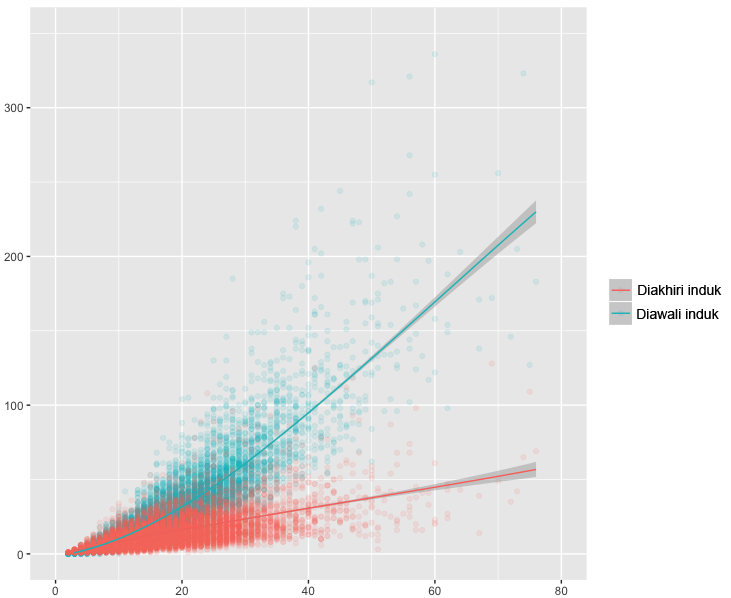
\includegraphics[width=1\linewidth] {pics/tulis_DLposneg.png} 
	\caption{Data ragam tulis}
	\label{fig:tulis_DLposneg} 
\end{subfigure}
%
\begin{subfigure}{.49\linewidth}
  \centering
  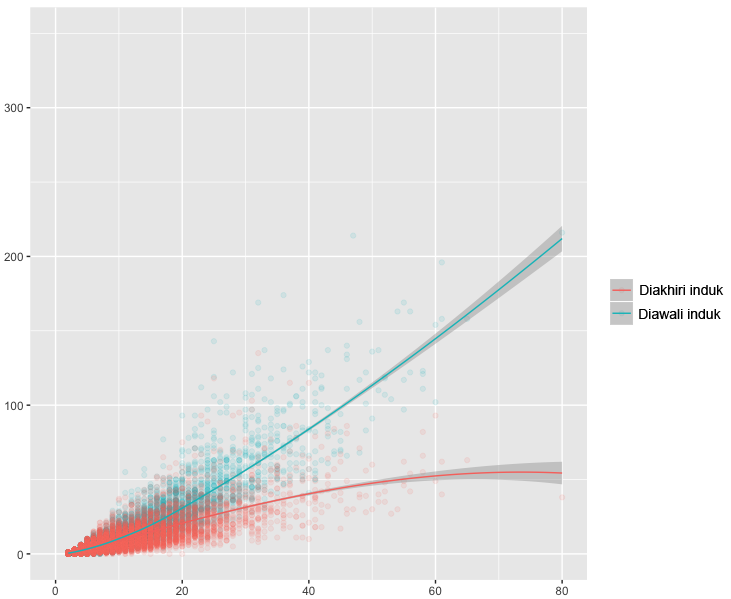
\includegraphics[width=1\linewidth]{pics/lisan_DLposneg.png} 
	\caption{Data ragam lisan}
	\label{fig:lisan_DLposneg} 
\end{subfigure}

\caption{Grafik nilai DL positif dan negatif data ragam tulis dan lisan}
\label{fig:DL_posneg}
\end{figure}


Pada bagian pertama analisis nilai DL positif dan negatif (\pic~\ref{fig:tulis_DLposneg}) dan \pic~\ref{fig:lisan_DLposneg}), kedua jenis nilai didapatkan dengan memisahkan total nilai dependensi positif dan negatif pada setiap kalimat. Nilai DL positif dan negatif ini memberikan gambaran kasus tautan akar atau induk dengan konstituen terikat secara general dan berkontribusi untuk membentuk asumsi kecenderungan karakteristik bahasa dilihat dari posisi induknya \citep{wang2017effects}. Berdasarkan \pic~\ref{fig:tulis_DLposneg} dan \pic~\ref{fig:lisan_DLposneg}, kedua korpus data menunjukkan garis regresi tautan dependensi positif yang jauh berada di atas garis regresi tautan dependensi negatif dan pada ujaran dengan jumlah konstituen yang semakin banyak, jarak antara keduanya semakin besar. Seperti yang dijelaskan sebelumnya, nilai DL cukup sensitif terhadap panjang kalimat dan keduanya memiliki hubungan linear. Dalam sebuah ujaran, perbandingan jumlah bentuk relasi induk sebelum dan sesudah konstituen terikat saling berkaitan. Hal ini berarti ada pola kecenderungan preferensi terhadap hubungan akar atau induk sebelum konstituen terikat (\textit{head-initial}) dan menandakan kesesuaian data observasi dengan tata bahasa yang berlaku. Namun, pada grafik nilai DL ragam lisan (\pic~\ref{fig:lisan_DLposneg}), garis regresi tautan dependensi negatif menunjukkan adanya kurva parabola terbka kebawah sehingga muncul asumsi adanya nilai tertinggi atau ambang batas (\textit{threshold}) terhadap nilai DL negatif pada korpus data ragam lisan. Berdasarkan korpus data yang terkumpul, dugaan ambang batas tautan dependensi negatif ini menandakan bahwa mulai panjang kalimat tertentu, total tautan dependensi negatif dalam sebuah kalimat mungkin tidak akan melebihi nilai tertentu juga. 

\begin{figure}
\centering

\begin{subfigure}{.4\linewidth}
  \centering
  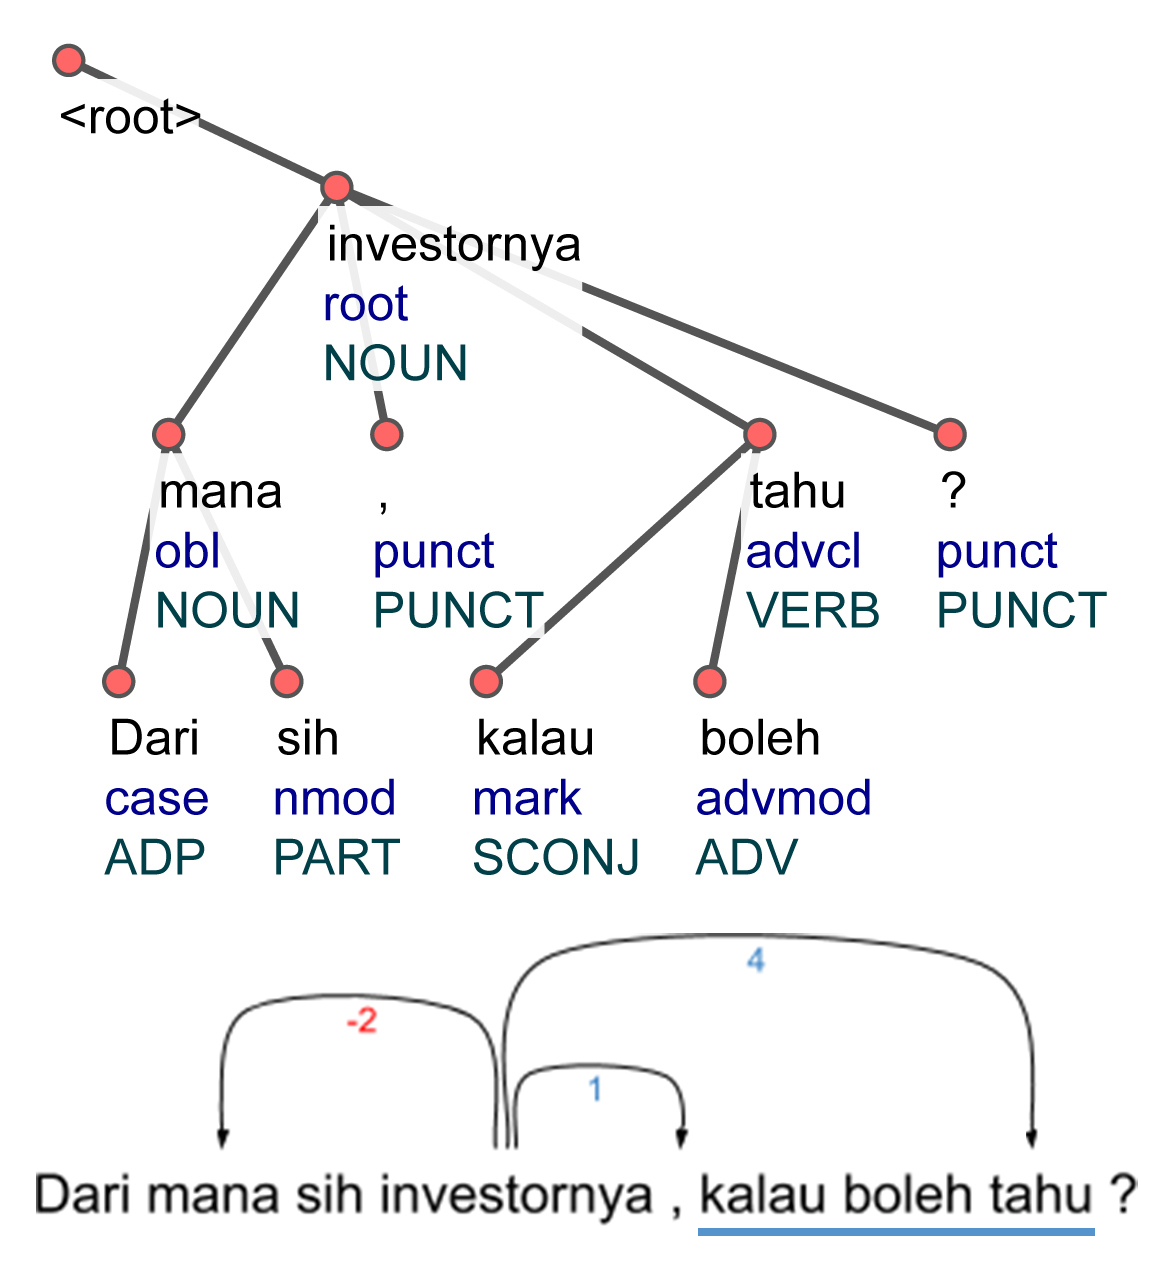
\includegraphics[width=1\linewidth] {pics/ls1436.jpg} 
	\caption{L\textit{akar}a}
	\label{fig:ls1436} 
\end{subfigure}
%
\begin{subfigure}{.58\linewidth}
  \centering
  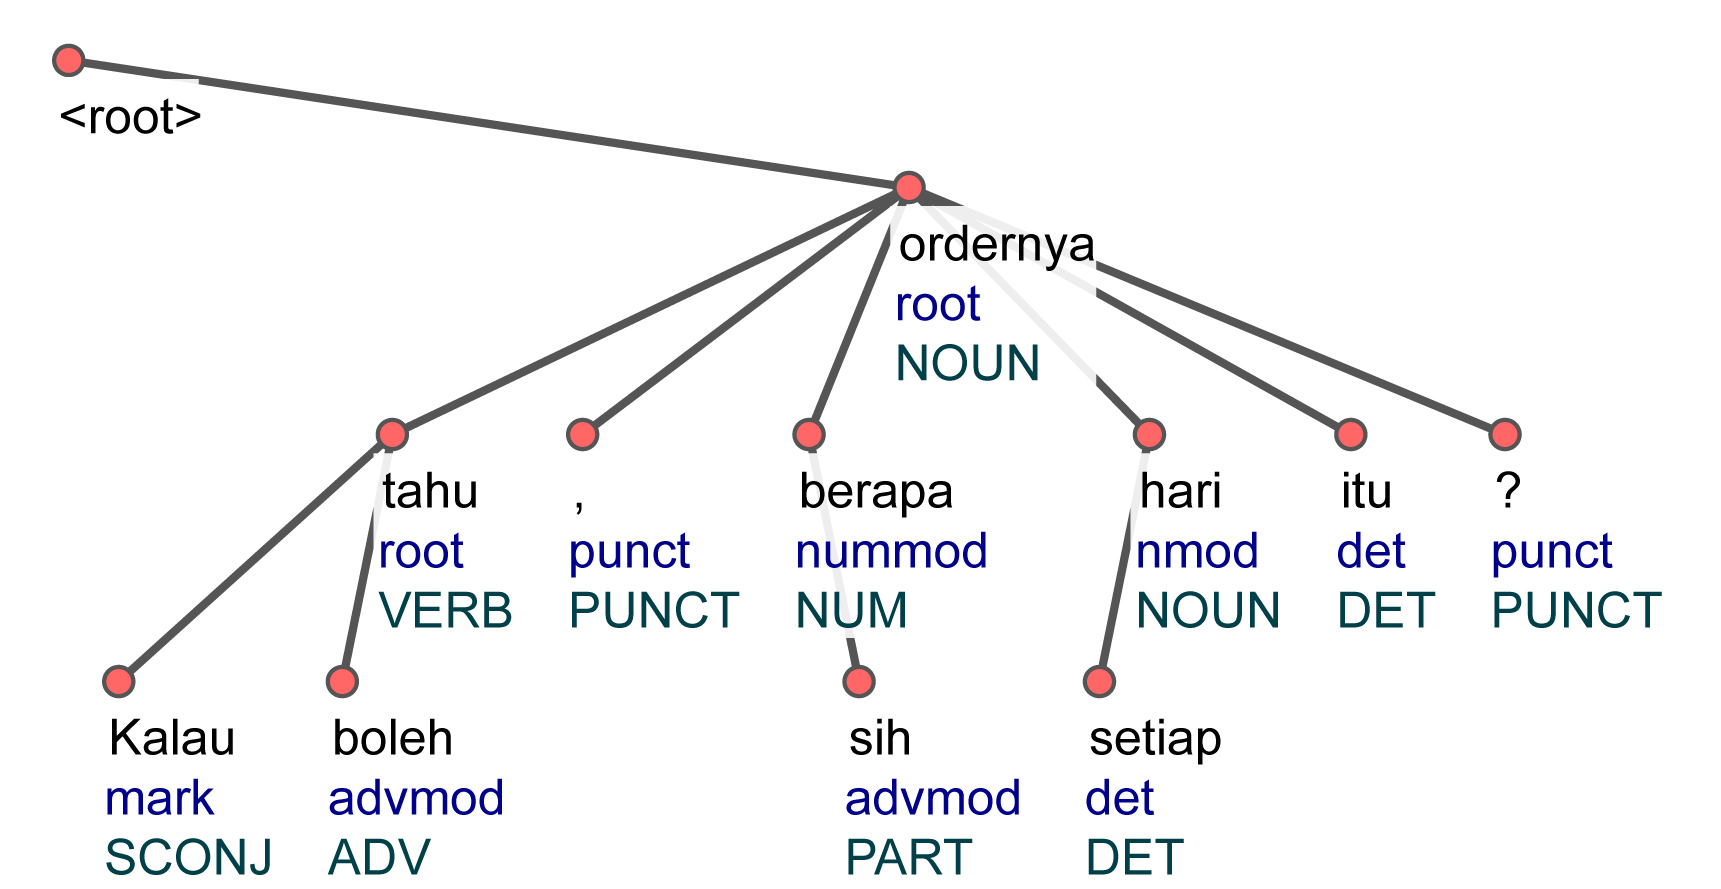
\includegraphics[width=1\linewidth]{pics/ls1460.jpg} 
	\caption{L\textit{akar}b}
	\label{fig:ls1460} 
\end{subfigure}

\caption{Contoh perbedaan penempatan klausa pada data ragam lisan}
\label{fig:akarcontoh}
\end{figure}


\pic~\ref{fig:ls1436} dan \pic~\ref{fig:ls1460} merupakan perbandingan kedua kalimat yang ditemukan pada korpus data ragam lisan. Kedua diagram pohon dependensi ini memberikan ilustrasi perbedaan letak akar dan klausa serta dampaknya terhadap nilai dependensi. Klausa terikat 'kalau boleh tahu' pada kalimat L\textit{akar}a (\pic~\ref{fig:ls1436}) dan L\textit{akar}b (\pic~\ref{fig:ls1460}) berada pada posisi yang berbeda namun tidak mengubah makna ujaran. Contoh serupa juga sempat dijabarkan oleh \cite{sneddon2010indonesian} dalam buku \textit{Indonesian Reference Grammar} Pada kalimat L\textit{akar}b, konstituen-konstiuen yang membentuk klausa 'kalau boleh tahu' secara kolektif memiliki relasi dependensi utama negatif terhadap akar 'ordernya'. Sesuai dengan bentuk relasi induk dan konstituen terikat berdasarkan teori dependensi yang dijabarkan oleh \cite{tesniere1959elements}, klausa terikat pada posisi awal ujaran ini harus disimpan dalam memori kerja terlebih dahulu hingga akar direalisasikan. Hal in berkebalikan dengan L\textit{akar}a yang dapat diproses langsung karena akar sudah direalisasikan terlebih dahulu. 

\begin{figure}
\centering

\begin{subfigure}{.49\linewidth}
  \centering
  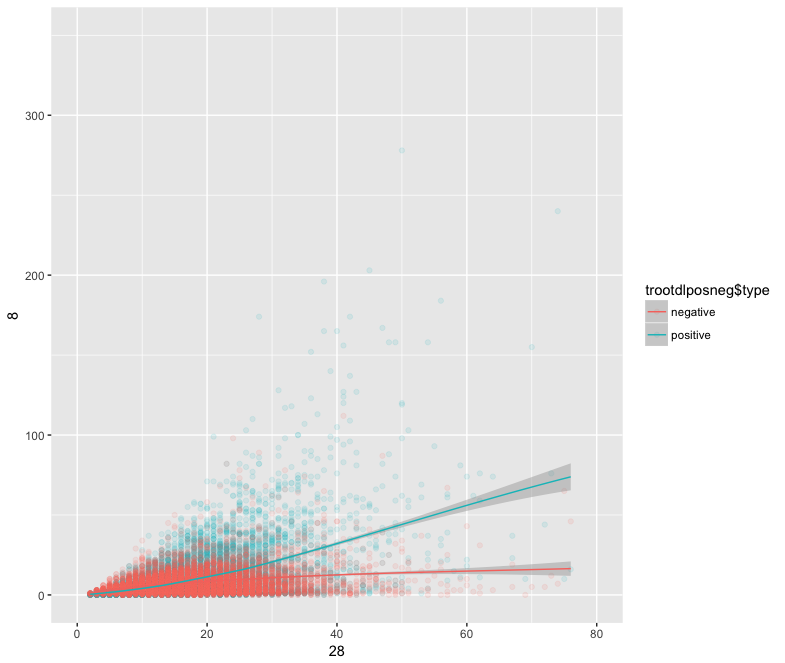
\includegraphics[width=1\linewidth] {pics/tulisroot_DLposneg.png} 
	\caption{Data ragam tulis}
	\label{fig:tulisroot_DLposneg} 
\end{subfigure}
%
\begin{subfigure}{.49\linewidth}
  \centering
  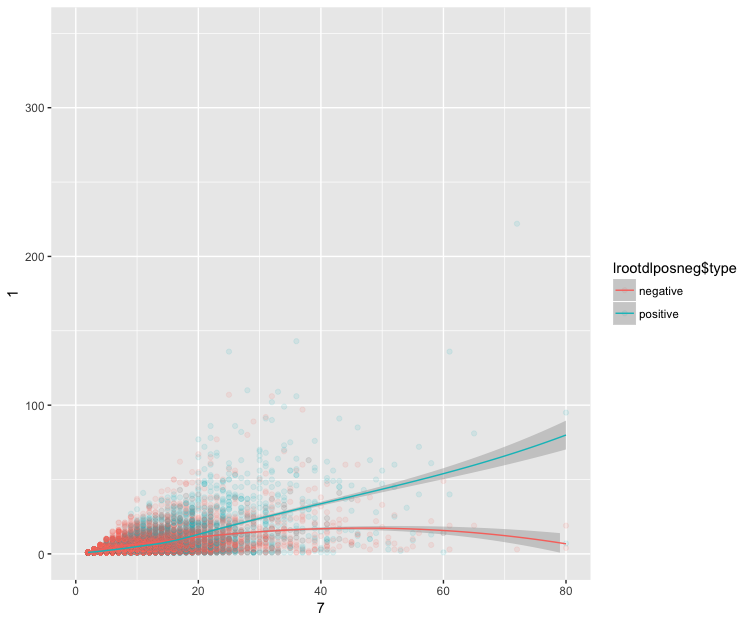
\includegraphics[width=1\linewidth]{pics/lisanroot_DLposneg.png} 
	\caption{Data ragam lisan}
	\label{fig:lisanroot_DLposneg} 
\end{subfigure}

\caption{Grafik nilai DL positif dan negatif pada simpai pusat data ragam tulis dan lisan}
\label{fig:rootDL_posneg}
\end{figure}

Bagian kedua analisis nilai DL positif dan negatif berkaitan dengan valensi sebuah kata sehubungan dengan contoh penempatan klausa terikat 'kalau boleh tahu' di atas (\pic~\ref{fig:akarcontoh}). Sesuai dengan batasan penelitian ini, bagian analisis ini difokuskan hanya pada simpai pusat dengan kelas kata akar berupa kata kerja atau verba. \pic~\ref{fig:tulisroot_DLposneg} dan \pic~\ref{fig:lisanroot_DLposneg} merupakan grafik nilai DL positif dan negatif yang didapat hanya pada simpai pusat ujaran dengan akar berupa verba. Ujaran dengan akar verbal ditemukan sebanyak 84,67\% atau sebanyak 7879 ujaran pada data ragam tulis dan 69,26\% atau sebanyak 7070 ujaran pada data ragam lisan. Mayoritas frekuensi kemunculan akar verbal ini dianalisis untuk melihat bagaimana penutur menyusun informasi utama dengan melihat tautan-tautan dependensi utama (simpai pusat). Sehingga, semua klausa yang mungkin terikat pada simpai cabang dianggap mengikuti induknya seperti pada contoh uraian relasi klausa 'kalau boleh tahu' dan akarnya di atas (\pic~\ref{fig:akarcontoh). \pic~\ref{fig:rootDL_posneg} menunjukkan adanya konsistens pada level tautan dependensi utama dan keseluruhan ujaran. Grafik ini memperlihatkan bahwa penutur juga cenderung memilih untuk menekan penggunaan bentuk relasi induk setelah konstituen terikatnya. Serupa dengan \pic~\ref{fig:DL_posneg}, terutama pada data ragam lisan, garis regresi nilai DL negatif mengindikasikan adanya ambang batas pada nilai tertentu. 	

%%-----------------------------------------------------------------------------%
\subsection{Temuan 6: Penempatan akar verbal dan klausa bebas utama di awal ujaran tanpa mengurangi valensi verbal}
%%-----------------------------------------------------------------------------%
Penempatan akar dan/atau klausa bebas utama di awal ujaran tanpa mengurangi valensi verbal cukup umum ditemukan pada kedua korpus data. Penempatan akar verbal pada posisi pertama seperti kalimat T\textit{akar}a \pic~ref{fig:ts770} dan T\textit{akar}b \pic~ref{fig:ts7458} ditemukan pada korpus data ragam tulis klasifikasi kalimat pendek dan menengah. Sebaliknya, penempatan akar di posisi pertama tanpa mengurangi valensi verbal tersebut sangat jarang ditemukan pada data ragam lisan.

\begin{figure}
\centering

\begin{subfigure}{.42\linewidth}
  \centering
  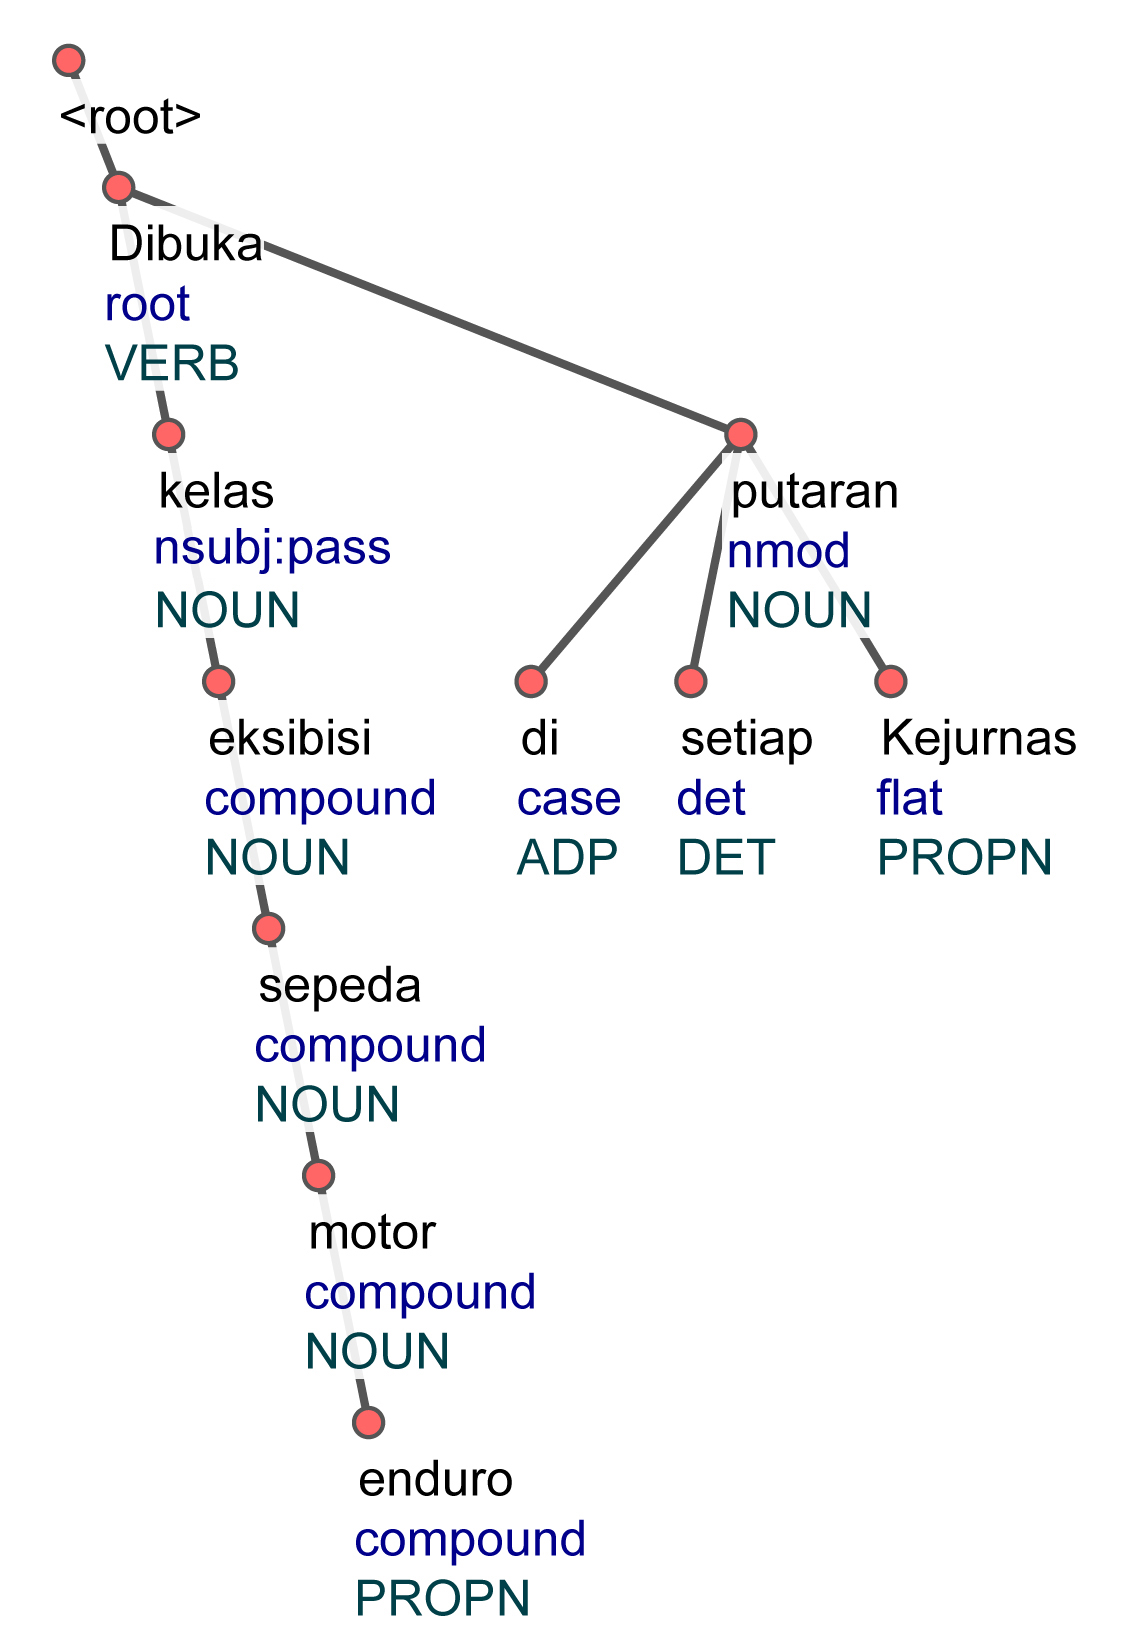
\includegraphics[width=1\linewidth] {pics/ts770.jpg} 
	\caption{T\textit{akar}a}
	\label{fig:ts770} 
\end{subfigure}
%
\begin{subfigure}{.57\linewidth}
  \centering
  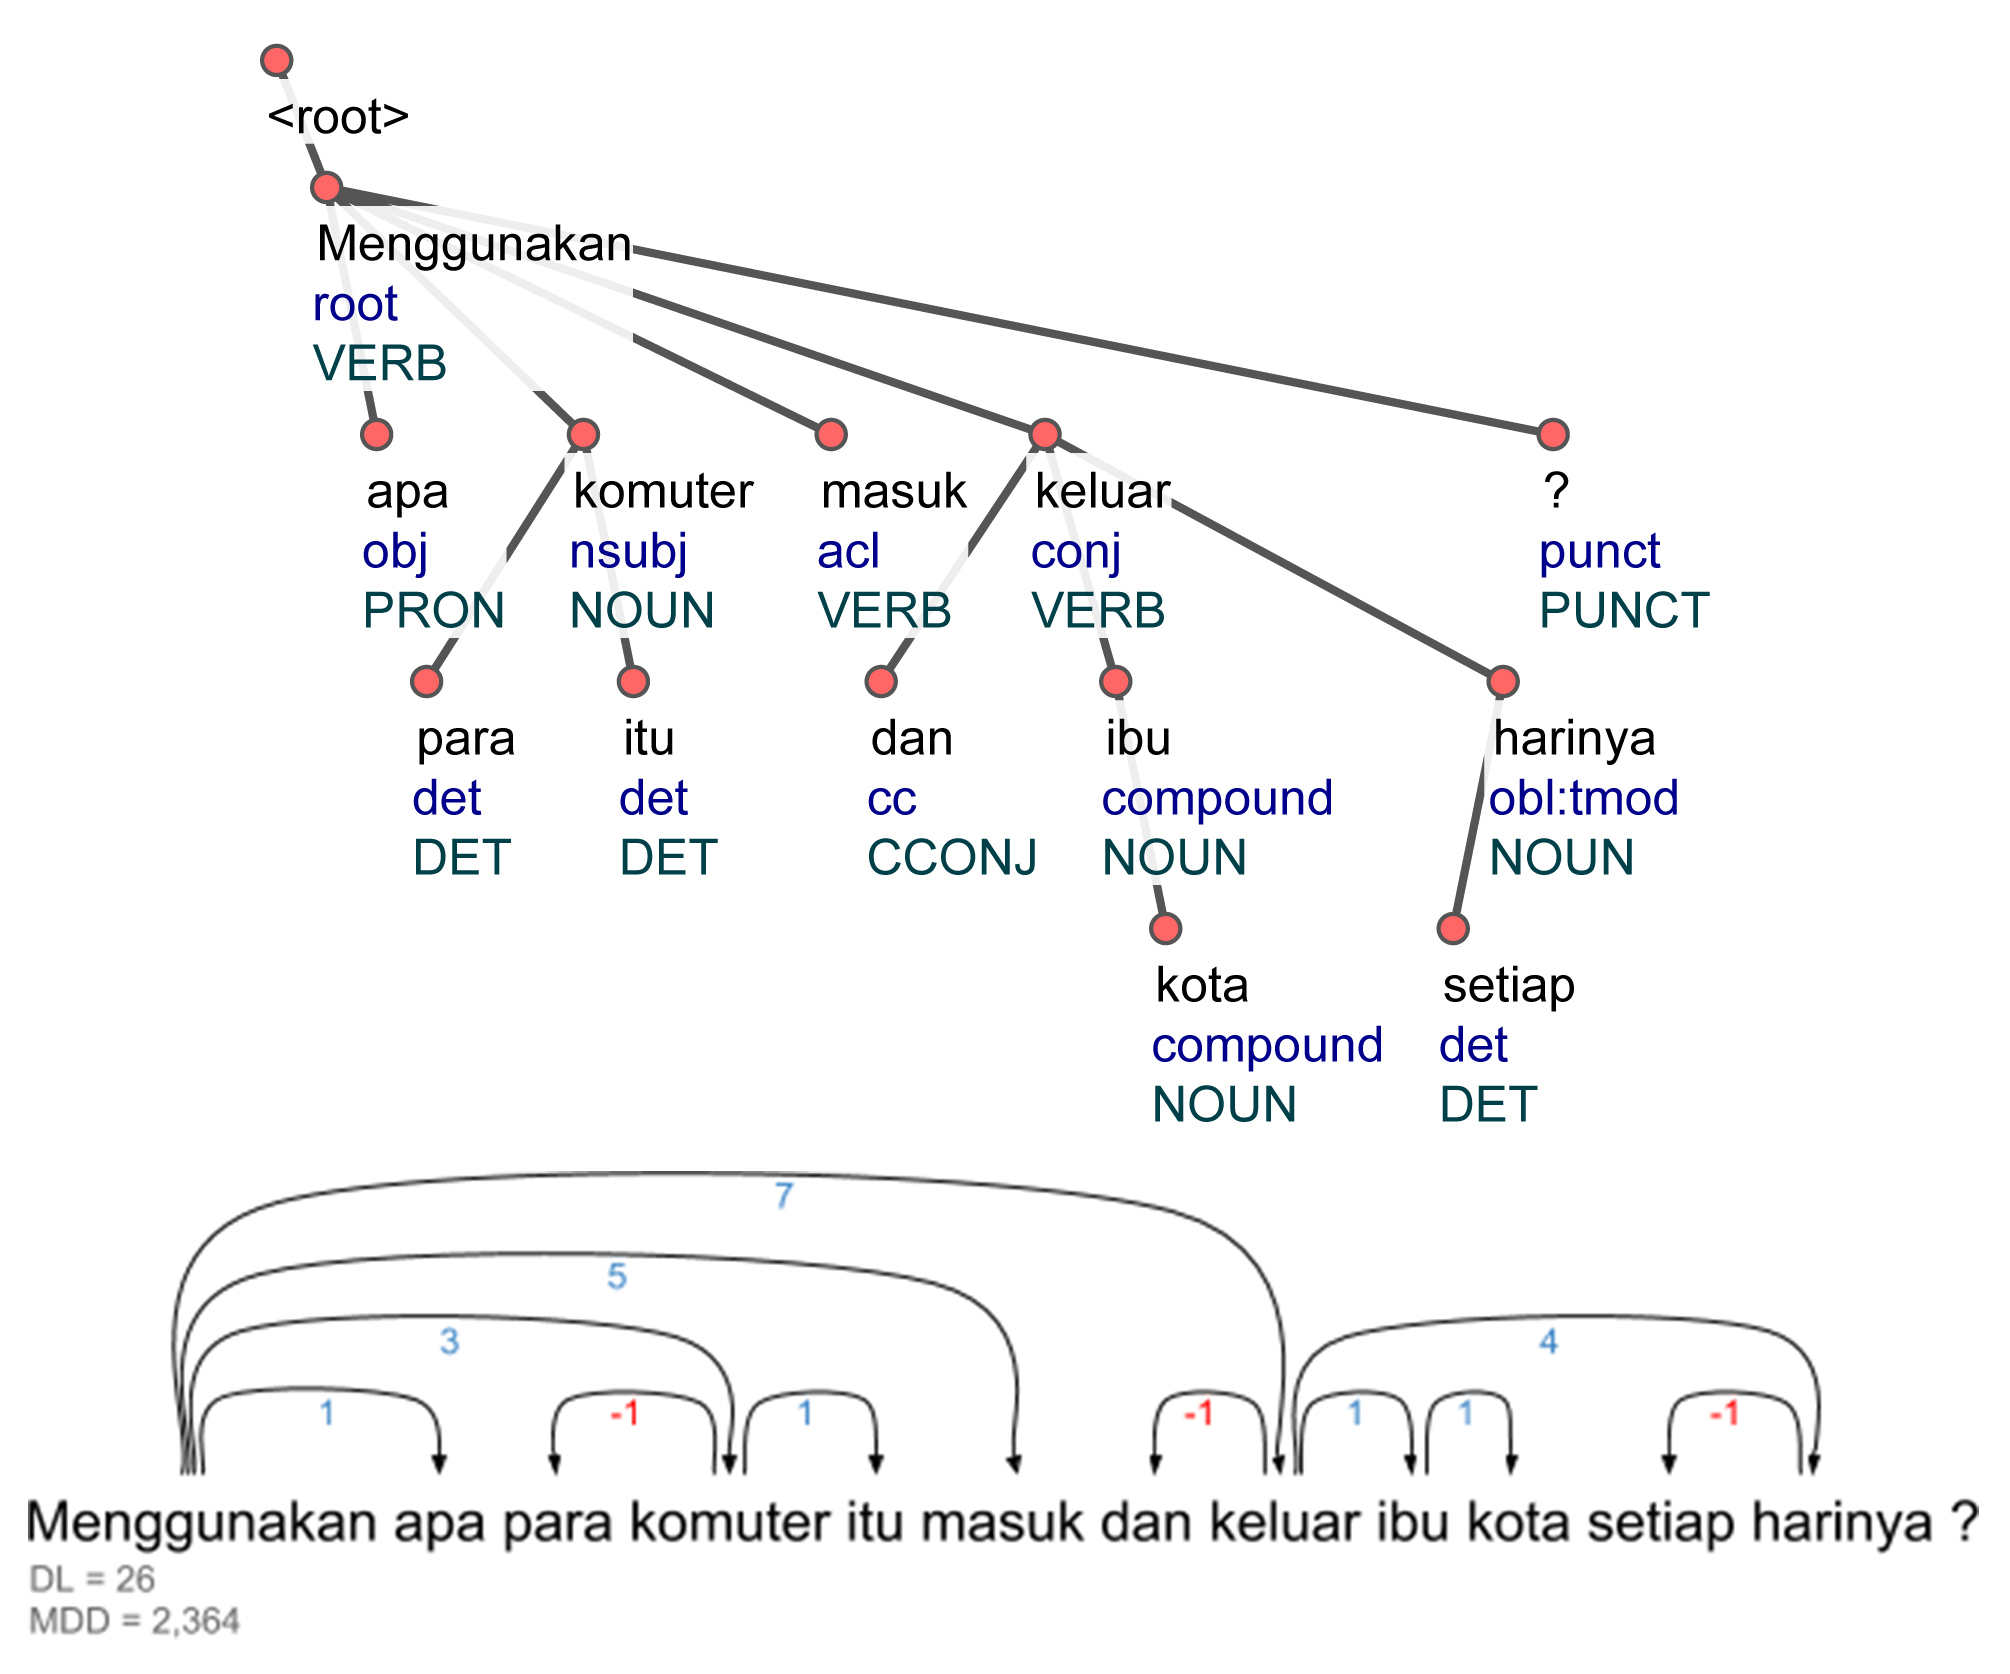
\includegraphics[width=1\linewidth]{pics/ts7458.jpg} 
	\caption{T\textit{akar}b}
	\label{fig:ts7458} 
\end{subfigure}
\caption{Contoh penempatan akar verbal dan klausa bebas utama di awal ujaran tanpa mengurangi valensi verbal pada data ragam tulis}
\label{fig:rootnovalensi}
\end{figure}

Pada ujaran T\textit{akar}a \pic~ref{fig:ts770}, akar verbal 'dibuka' tetap mengikat konstituen terikat obyek 'kelas'. Akar verbal 'dibuka' pada ujaran tersebut tergolong verba statif (keadaan) sehingga tidak diperlukan kemunculan aktor pelaku dalam kalimat terebut \cite{sneddon2010indonesian}. Serupa dengan ujaran T\textit{akar}a, akar verbal 'menggunakan' pada ujaran T\textit{akar}b \pic~ref{fig:ts7458} tetap mempertahankan valensi terhadap 'komuter' (aktor pelaku) dan 'apa' (pengganti obyek) namun konstruksinya tidak umum seperti halnya aktor pelaku mendahului verba dalam bahasa Indonesia. Contoh ini memberikan indikasi pemanfaatan kebebasan urutan kata dalam Bahasa Indonesia untuk menghindari bentuk relasi induk setelah konstituen terikat dan tetap merealisasikan akar seawal mungkin. Penempatan klausa bebas utama di awal ujaran lebih banyak ditemukan pada data ragam tulis dibandingkan ragam lisan. Penempatan klausa bebas utama di awal ujaran ini menyebabkan akar verbal secara otomatis tetap berada di awal tanpa mengurangi valensi akar verbal tersebut. Namun, karena jumlah konstituen yang panjang dan struktur ujaran dengan klausa-klausa yang lebih kompleks, posisi akar verbal umumnya tidak pada posisi pertama. Pada ujaran seperti ini, konstituen terikat berupa aktor pelaku umumnya direalisasikan sebelum akar verbal. Contoh strategi ini dapat dilihat pada kalimat T31b (\pic~\ref{fig:ts2081}) untuk data ragam tulis dan L31a (\pic~\ref{fig:ls1716}) untuk data ragam lisan.

%%-----------------------------------------------------------------------------%
\subsection{Temuan 7: Penempatan akar verbal dan klausa bebas di awal ujaran disertai pengurangan valensi verbal}
%%-----------------------------------------------------------------------------%
Sejumlah simpai pusat dalam kedua korpus data mengalami pengurangan valensi verbal yang mengakibatkan pengurangan panjang serta jarak dependensi. Ujaran seperti ini sangat jarang ditemui pada data ragam tulis, namun banyak ditemukan pada data ragam lisan, terutama pada klasifikasi kalimat pendek dan menengah. Strategi pengurangan valensi verbal ini banyak ditemukan disertai dengan penempatan akar di awal ujaran seperti pada temuan sebelumnya. Hal ini juga berkaitan dengan temuan pengaruh panjang kalimat di atas yang menandakan kecenderungan jumlah konstituen yang lebih sedikit pada data ragam lisan.  

\begin{figure}
\centering

\begin{subfigure}{.49\linewidth}
  \centering
  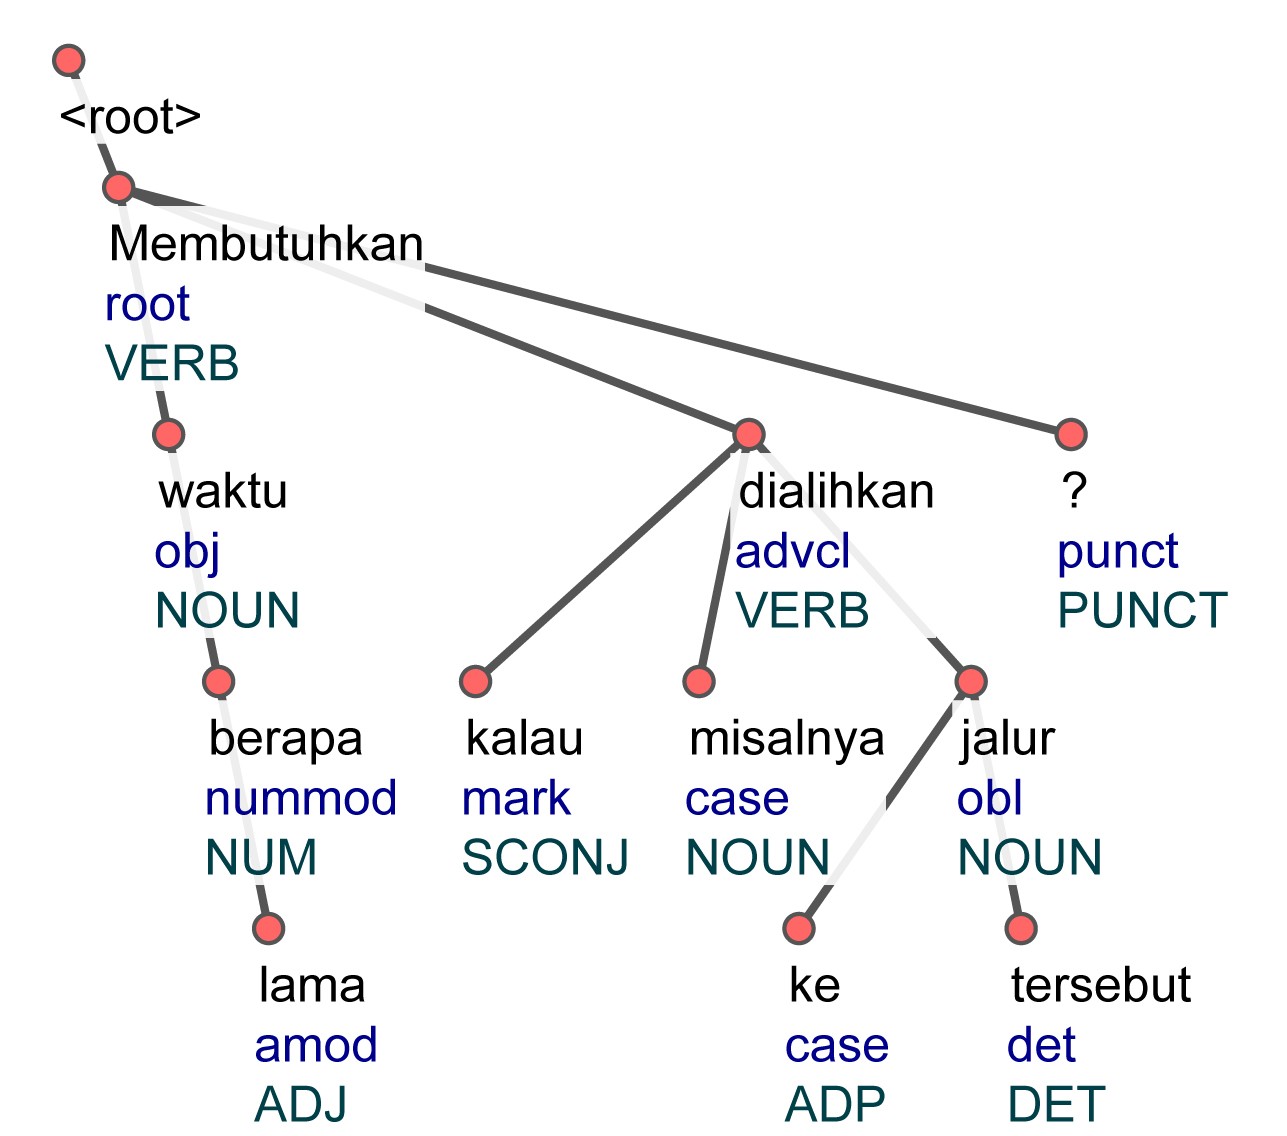
\includegraphics[width=1\linewidth] {pics/ls4820.jpg} 
	\caption{L\textit{akar}c}
	\label{fig:ls4820} 
\end{subfigure}
%
\begin{subfigure}{.41\linewidth}
  \centering
  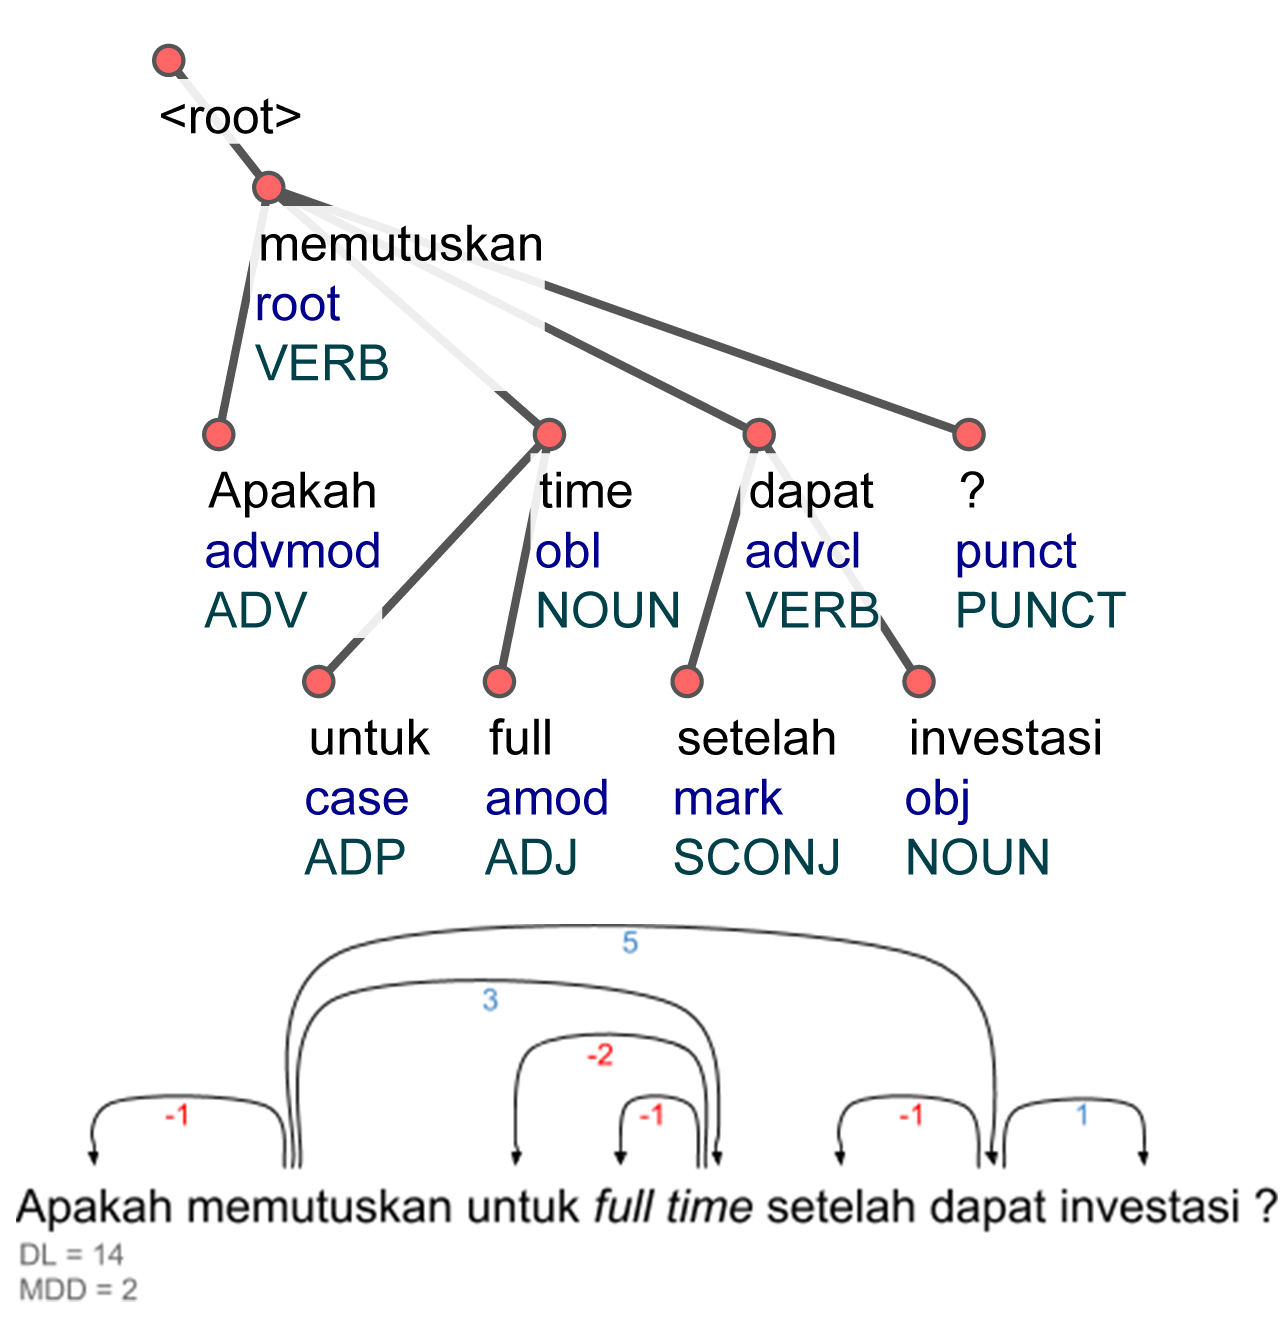
\includegraphics[width=1\linewidth]{pics/ls1435.jpg} 
	\caption{L\textit{akar}d}
	\label{fig:ls1435} 
\end{subfigure}
\caption{Contoh penempatan akar verbal dan klausa bebas utama di awal ujaran tanpa mengurangi valensi verbal pada data ragam tulis}
\label{fig:rootvalensi}
\end{figure}

Pada ujaran L\textit{akar}c (\pic~\ref{fig:ls4820}, akar verbal 'membutuhkan' umumnya memiliki valensi sebanyak dua konstituen, yaitu aktor pelaku dan obyek atau '$X$ membutuhkan $Y$'. Kata ini mengalami pengurangan valensi akar verbal sehingga yang muncul hanya obyek nomina 'waktu'. Begitu pula dengan ujaran L\textit{akar}d (\pic~\ref{fig:ls1435} yang juga mengalami pengurangan valensi akar verbal berupa aktor pelaku. Ujaran L\textit{akar}e (\pic~\ref{fig:ls1265}) merupakan contoh lain yang mengalami pengurangan valensi verbal berupa aktor pelaku dan/atau pronomina pada klausa bebas utama maupun klausa terikatnya. Ujaran ini tidak memunculkan pelengkap pada klausa '$X$ mengganti alat' dan/atau pada klausa 'supaya $X$ tidak berebut ikan'.

\begin{figure}
	\centering 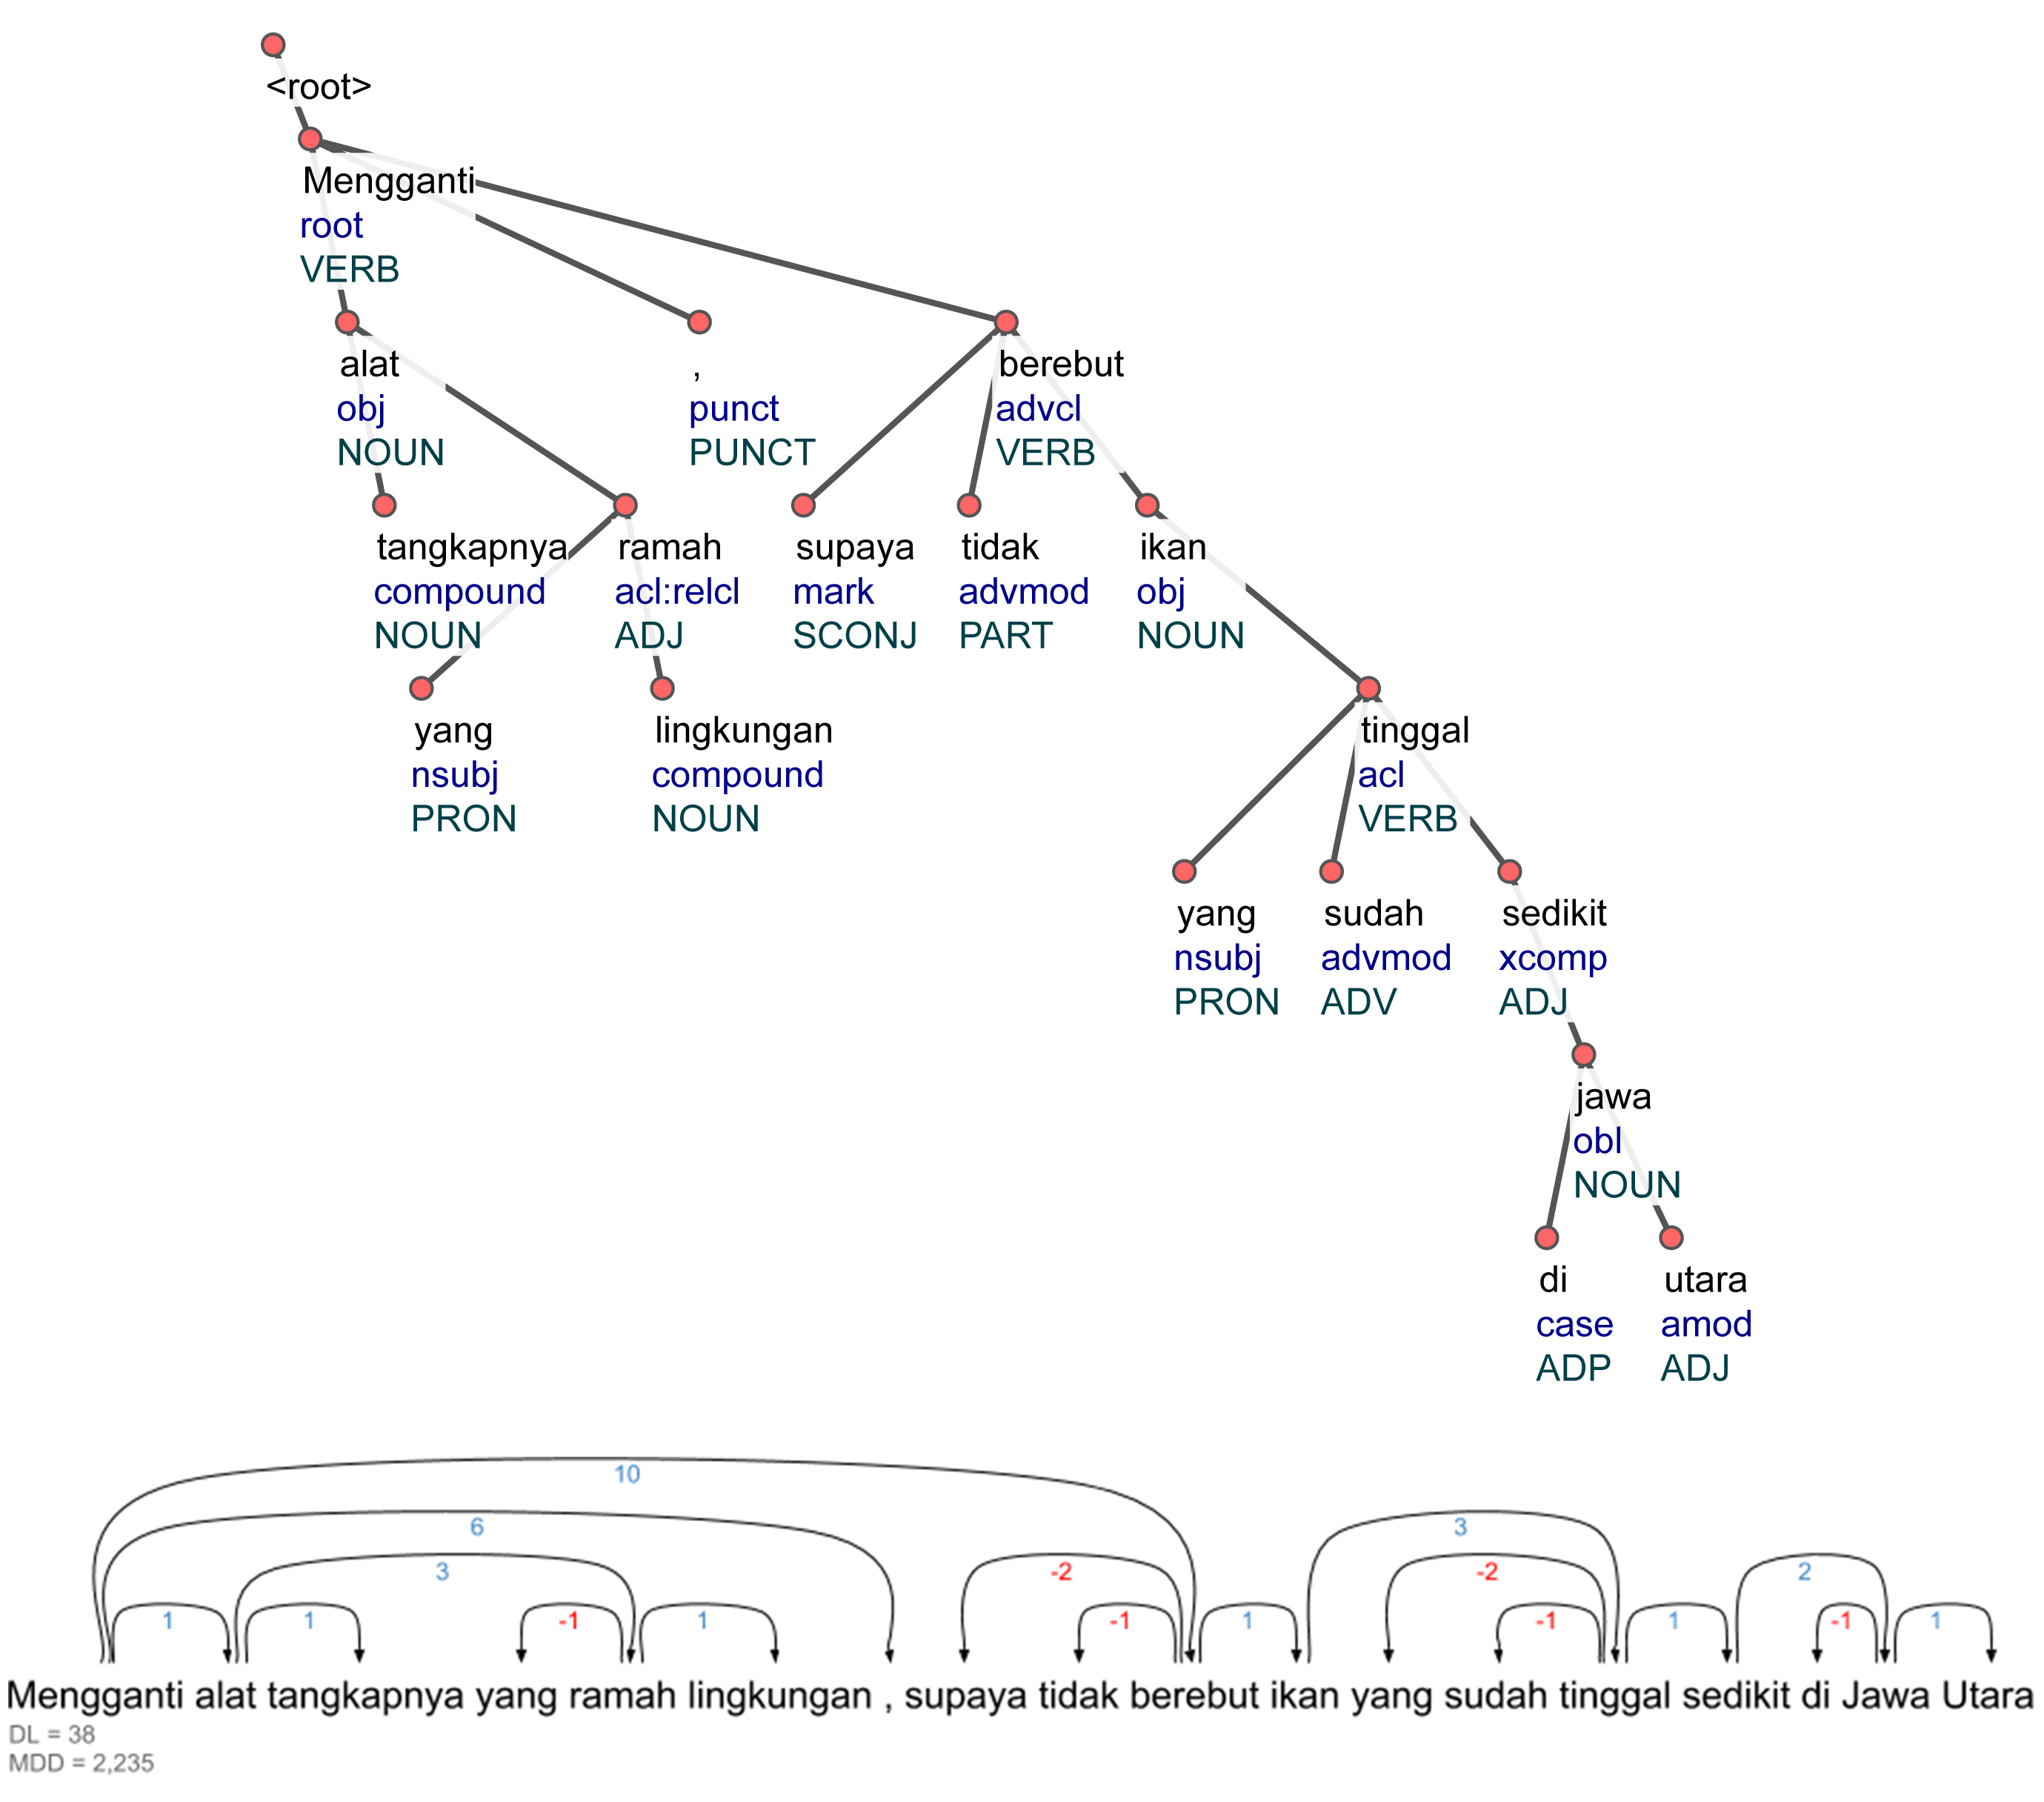
\includegraphics[width=0.9
	\textwidth] {pics/ls1265.jpg} 
	\caption{Ujaran L\textit{akar}e pada data ragam lisan}
	\label{fig:ls1265} 
\end{figure}

Strategi ujaran seperti ini muncul dalam wacana-wacana di mana konstituen yang direduksi dari valensi verbal sudah terlebih dahulu direalisasikan di ujaran-ujaran sebelumnya atau sudah dimengerti bersama tanpa harus direalisasikan dalam kalimat tertentu. Batasan penelitian ini hanya pada tataran kalimat sehingga tidak menganalisis hubungan dependensi yang terbentuk antarkalimat. Namun, asumsi ini menimbulkan pertanyaan untuk analisis dependensi lanjutan pada tataran wacana yaitu bagaimana dan sejauh mana tautan dependensi yang terbentuk antarkalimat sehingga memungkinkan adanya pengurangan valensi verbal pada kalimat tertentu?

%%-----------------------------------------------------------------------------%
\subsection{Diskusi temuan 6 dan 7}
%%-----------------------------------------------------------------------------%
Bagian analisis ini mencoba menjawab pertanyaan terkait arah tautan dependensi (\textit{head directionality}) dan pengurangan valensi akar verbal pada simpai pusat. Pengurangan konstituen dalam ujaran atau preferensi terhadap kalimat pendek terutama pada ragam lisan tidak selalu berarti menandakan adanya pengurangan valensi sebuah konstituen. Pada penelitian-penelitian terdahulu banyak dilakukan eksplorasi terhadap reduksi leksikal lain seperti konjungsi, partikel, ataupun kata-kata lain yang bersifat berulang atau \textit{repetitive} (\citealp{jaeger2006redundancy, gildea2015human}). Penelitian ini memfokuskan pengurangan valensi pada simpai pusat dengan akar verbal yang merupakan tipe akar yang paling banyak ditemukan pada kedua korpus data. 

Seperti yang dibahas pada bab sebelumnya, arah tautan dependensi dapat menyebabkan nilai dependensi tersebut menjadi positif atau negatif. Nilai positif yang menandakan bentuk relasi induk sebelum konstituen terikat (\textit{head-initial}). Berdasarkan aturan struktur frasa dalam tata bahasa yang ada (\citealp{kridalaksana2002struktur, sneddon2010indonesian}), terdapat indikasi bahwa bahasa Indonesia tergolong bahasa yang memilih bentuk \textot{head-initial} dibandingkan \textit{head-final}. Namun, belum ada penelitian dengan skala cukup besar yang dapat memberikan informasi ini dengan memanfaatkan data ujaran nyata (\textit{real utterance}) karena penerapannya dalam ujaran nyata dapat bersifat tidak gramatikal. Bentuk \textit{head-intial} tidak selalu menjadi preferensi pada semua bahasa karena beberapa bahasa memiliki aturan tata bahasa yang menuntut induk muncul setelah konstituen terikat atau \textit{head-final}. Meskipun belum ada konvensi dan bukti empiris yang menunjukkan bahwa bentuk ini lebih memudahkan proses memori kerja, \cite{futrell2015large} menunjukkan bukti empiris bahwa bahasa-bahasa yang cenderung menggunakan bentuk relasi ini memiliki tingkat pengurangan jarak dependensi (DLM) lebih tinggi dibandingkan bahasa-bahasa yang cenderung menggunakan bentuk relasi induk setelah konstituen terikat (\textit{head-final}). 

Didukung oleh hasil penelitian ini, bahasa Indonesia menunjukkan kecenderungan terhadap bentuk \textit{head-initial} pada simpai pusat maupun keseluruhan ujaran (antarkonstituen yang memiliki tautan langsung maupun antarkonstituen pada simpai pusat) yang ditandai oleh konsistensi nilai DL positif yang semakin tinggi terutama pada ujaran yang memiliki jumlah konstituen lebih banyak. Temuan ini menandakan konsistensi untuk menekan nilai DL negatif pada level struktur yang berbeda dan mengindikasikan preferensi head-initial di segala kondisi. Secara otomatis pergerakan nilai DL positif yang semakin tinggi mengakibatkan penekanan bentuk \textit{head-final} yang ditandai oleh nilai DL negatif. Bahkan, pada ragam lisan ditemukan indikasi adanya ambang batas terhadap frekuensi bentuk \textit{head-final}. Temuan ini memunculkan asumsi bahwa dalam bahasa Indonesia, ujaran dengan kecenderungan bentuk relasi induk sebelum konstituen terikat lebih banyak digunakan penutur dan menunjukkan indikasi bahwa bentuk ini lebih mudah dimengerti. Penelitian lebih lanjut dibutuhkan untuk menunjukkan bukti empiris untuk mendukung hipotesis ini dan mengukur seberapa bentuk relasi \textit{head-initial} memudahkan proses memori kerja. 

Analisis kualitatif untuk melihat lebih dalam bagaimana strategi yang mendukung preferensi \textit{head-initial} ini dilakukan dengan meninjau simpai-simpai pusat ujaran yang memiliki akar verbal pada kedua korpus. Secara umum, ditemukan dua strategi terkait arah dan valensi akar verbal yaitu, penempatan akar dan klausa bebas utama di awal ujaran dengan atau tanpa mengurangi valensi akar verbal. Penempatan akar dan klausa bebas utama di awal ujaran sangat umum ditemukan pada semua klasifikasi dalam korpus data ragam tulis. Namun, posisinya sedikit bergeser seiring dengan semakin banyaknya jumlah konstituen. Hal ini dikarenakan penempatan klausa bebas utama yang hampir selalu di posisi awal pada data ragam tulis. Sementara, pengurangan valensi akar verbal hampir tidak ditemukan pada data ragam tulis yang mungkin disebabkan karena karakter wacananya lebih formal dibandingkan dengan ragam lisan. Pengurangan valensi ini secara langsung berakibat pada pengurangan konstituen secara keseluruhan, sehingga dapat dikaitkan dengan temuan adanya preferensi untuk kalimat dengan jumlah konstituen yang lebih sedikit pada ragam lisan pada klasifikasi kalimat pendek dan menengah. Pengurangan valensi akar verbal ini sering disertai dengan penempatan posisi akar di awal ujaran ragam lisan namun hampir tidak ditemukan pada klasifikasi kalimat panjang. 

Temuan yang menarik adalah pada klasifikasi kalimat pendek dan menengah data ragam tulis maupun lisan, penempatan akar verbal yang aktor pelaku dalam valensinya sering berada pada posisi pertama baik dengan atau tanpa pengurangan valensi akar verbal (terutama aktor pelaku). Namun, mulai pada panjang kalimat tertentu, penempatan akar verbal yang mengikat aktor pelaku dalam valensinya tidak ditemukan pada posisi pertama dan aktor pelaku selalu direalisasikan sebelum akar verbal .Pengurangan valensi berupa aktor pelaku yang berupa kata penuh pada simpai dengan akar verbal tidak ditemukan apabila klausa utama didahului klausa lain, namun pengurangan valensi aktor pelaku yang berupa pronomina pengganti pada simpai dengan induk verbal ditemukan apabila klausa utama juga mengalami pengurangan valensi aktor pelaku. Untuk meninjau lebih dalam signifikansi temuan pengurangan valensi pada kondisi tersebut memerlukan pendekatan kuantitatif yang menuntut adanya sumber daya kamus atau leksikon valensi. Tinjauan lebih lanjut mengenai temuan-temuan ini dapat memberikan gambaran lebih dalam mengenai kognisi manusia terkait struktur ujaran yang dikonstruksi dan dapat memberikan masukan terhadap penggunaan tata bahasa yang memudahkan komunikasi serta proses memori kerja.

%%-----------------------------------------------------------------------------%
%\section{thesis.tex}
%%-----------------------------------------------------------------------------%
%Berkas ini berisi seluruh berkas Latex yang dibaca, jadi bisa dikatakan sebagai 
%berkas utama. Dari berkas ini kita dapat mengatur bab apa saja yang ingin 
%kita tampilkan dalam dokumen.
%
%
%%-----------------------------------------------------------------------------%
%\section{laporan\_setting.tex}
%%-----------------------------------------------------------------------------%
%Berkas ini berguna untuk mempermudah pembuatan beberapa template standar. 
%Anda diminta untuk menuliskan judul laporan, nama, npm, dan hal-hal lain yang 
%dibutuhkan untuk pembuatan template. 
%
%
%%-----------------------------------------------------------------------------%
%\section{istilah.tex}
%%-----------------------------------------------------------------------------%
%Berkas istilah digunakan untuk mencatat istilah-istilah yang digunakan. 
%Fungsinya hanya untuk memudahkan penulisan.
%Pada beberapa kasus, ada kata-kata yang harus selalu muncul dengan tercetak 
%miring atau tercetak tebal. 
%Dengan menjadikan kata-kata tersebut sebagai sebuah perintah \latex~tentu akan 
%mempercepat dan mempermudah pengerjaan laporan. 
%
%
%%-----------------------------------------------------------------------------%
%\section{hype.indonesia.tex}
%%-----------------------------------------------------------------------------%
%Berkas ini berisi cara pemenggalan beberapa kata dalam bahasa Indonesia. 
%\latex~memiliki algoritma untuk memenggal kata-kata sendiri, namun untuk 
%beberapa kasus algoritma ini memenggal dengan cara yang salah. 
%Untuk memperbaiki pemenggalan yang salah inilah cara pemenggalan yang benar 
%ditulis dalam berkas hype.indonesia.tex.
%
%
%%-----------------------------------------------------------------------------%
%\section{pustaka.tex}
%%-----------------------------------------------------------------------------%
%Berkas pustaka.tex berisi seluruh daftar referensi yang digunakan dalam 
%laporan. 
%Anda bisa membuat model daftar referensi lain dengan menggunakan bibtex.
%Untuk mempelajari bibtex lebih lanjut, silahkan buka 
%\url{http://www.bibtex.org/Format}. 
%Untuk merujuk pada salah satu referensi yang ada, gunakan perintah \bslash 
%cite, e.g. \bslash cite\{latex.intro\} yang akan akan memunculkan 
%\cite{latex.intro}
%
%
%%-----------------------------------------------------------------------------%
%\section{bab[1 - 6].tex}
%%-----------------------------------------------------------------------------%
%Berkas ini berisi isi laporan yang Anda tulis. 
%Setiap nama berkas e.g. bab1.tex merepresentasikan bab dimana tulisan tersebut 
%akan muncul. 
%Sebagai contoh, kode dimana tulisan ini dibaut berada dalam berkas dengan nama 
%bab4.tex. 
%Ada enam buah berkas yang telah disiapkan untuk mengakomodir enam bab dari 
%laporan Anda, diluar bab kesimpulan dan saran. 
%Jika Anda tidak membutuhkan sebanyak itu, silahkan hapus kode dalam berkas 
%thesis.tex yang memasukan berkas \latex~yang tidak dibutuhkan;  contohnya 
%perintah \bslash include\{bab6.tex\} merupakan kode untuk memasukan berkas 
%bab6.tex kedalam laporan.
%
